%Background image credits:https://commons.wikimedia.org/wiki/File:Votive_relief_of_the_goddess_Cybele_(4th_cent._B.C.)_at_the_National_Archaeological_Museum_of_Athens_on_22_July_2018.jpg George E. Koronaios, CC BY-SA 4.0, via Wikimedia Commons
%Background image credits:https://commons.wikimedia.org/wiki/File:Hemp_paper_in_Japan.jpg タバコはマーダー, CC BY-SA 4.0, via Wikimedia Commons
\documentclass[a4paper, 11pt, oneside, polutonikogreek, english]{article}
\usepackage[T1]{fontenc}
\usepackage{drm}
% Load encoding definitions (after font package)

\usepackage[dvipsnames]{xcolor}
\usepackage{eso-pic,graphicx}
\usepackage[top=55mm, bottom=25mm, outer=18mm, inner=18mm]{geometry}
\setlength{\columnsep}{90pt}
%\definecolor{customColor}{RGB}{253, 227, 54}

\usepackage{textalpha}

\usepackage{listings}
\lstset{basicstyle=\ttfamily}
\usepackage{pdflscape}

% Babel package:
\usepackage[english]{babel}

% With XeTeX$\$LuaTeX, load fontspec after babel to use Unicode
% fonts for Latin script and LGR for Greek:
\ifdefined\luatexversion \usepackage{fontspec}\fi
\ifdefined\XeTeXrevision \usepackage{fontspec}\fi

% ``Lipsiakos" italic font `cbleipzig`:
\newcommand*{\lishape}{\fontencoding{LGR}\fontfamily{cmr}%
		       \fontshape{li}\selectfont}
\DeclareTextFontCommand{\textli}{\lishape}

\usepackage{booktabs}
\usepackage{graphicx}
\setlength{\emergencystretch}{15pt}
\graphicspath{ {./ } }
\usepackage[figurename=]{caption}
\usepackage{float}
\usepackage{fancyhdr}
\usepackage{microtype}

\usepackage{setspace}
\onehalfspacing

% change color of text, example replace all \color{Goldenrod} with \color{lightgray}

\makeatletter % change only the display of \thepage, but not \thepage itself:
\patchcmd{\ps@plain}{\thepage}{\color{Black}{\thepage}}{}{}
\makeatother

\color{Black}

\begin{document}
\onecolumn
\AddToShipoutPictureBG{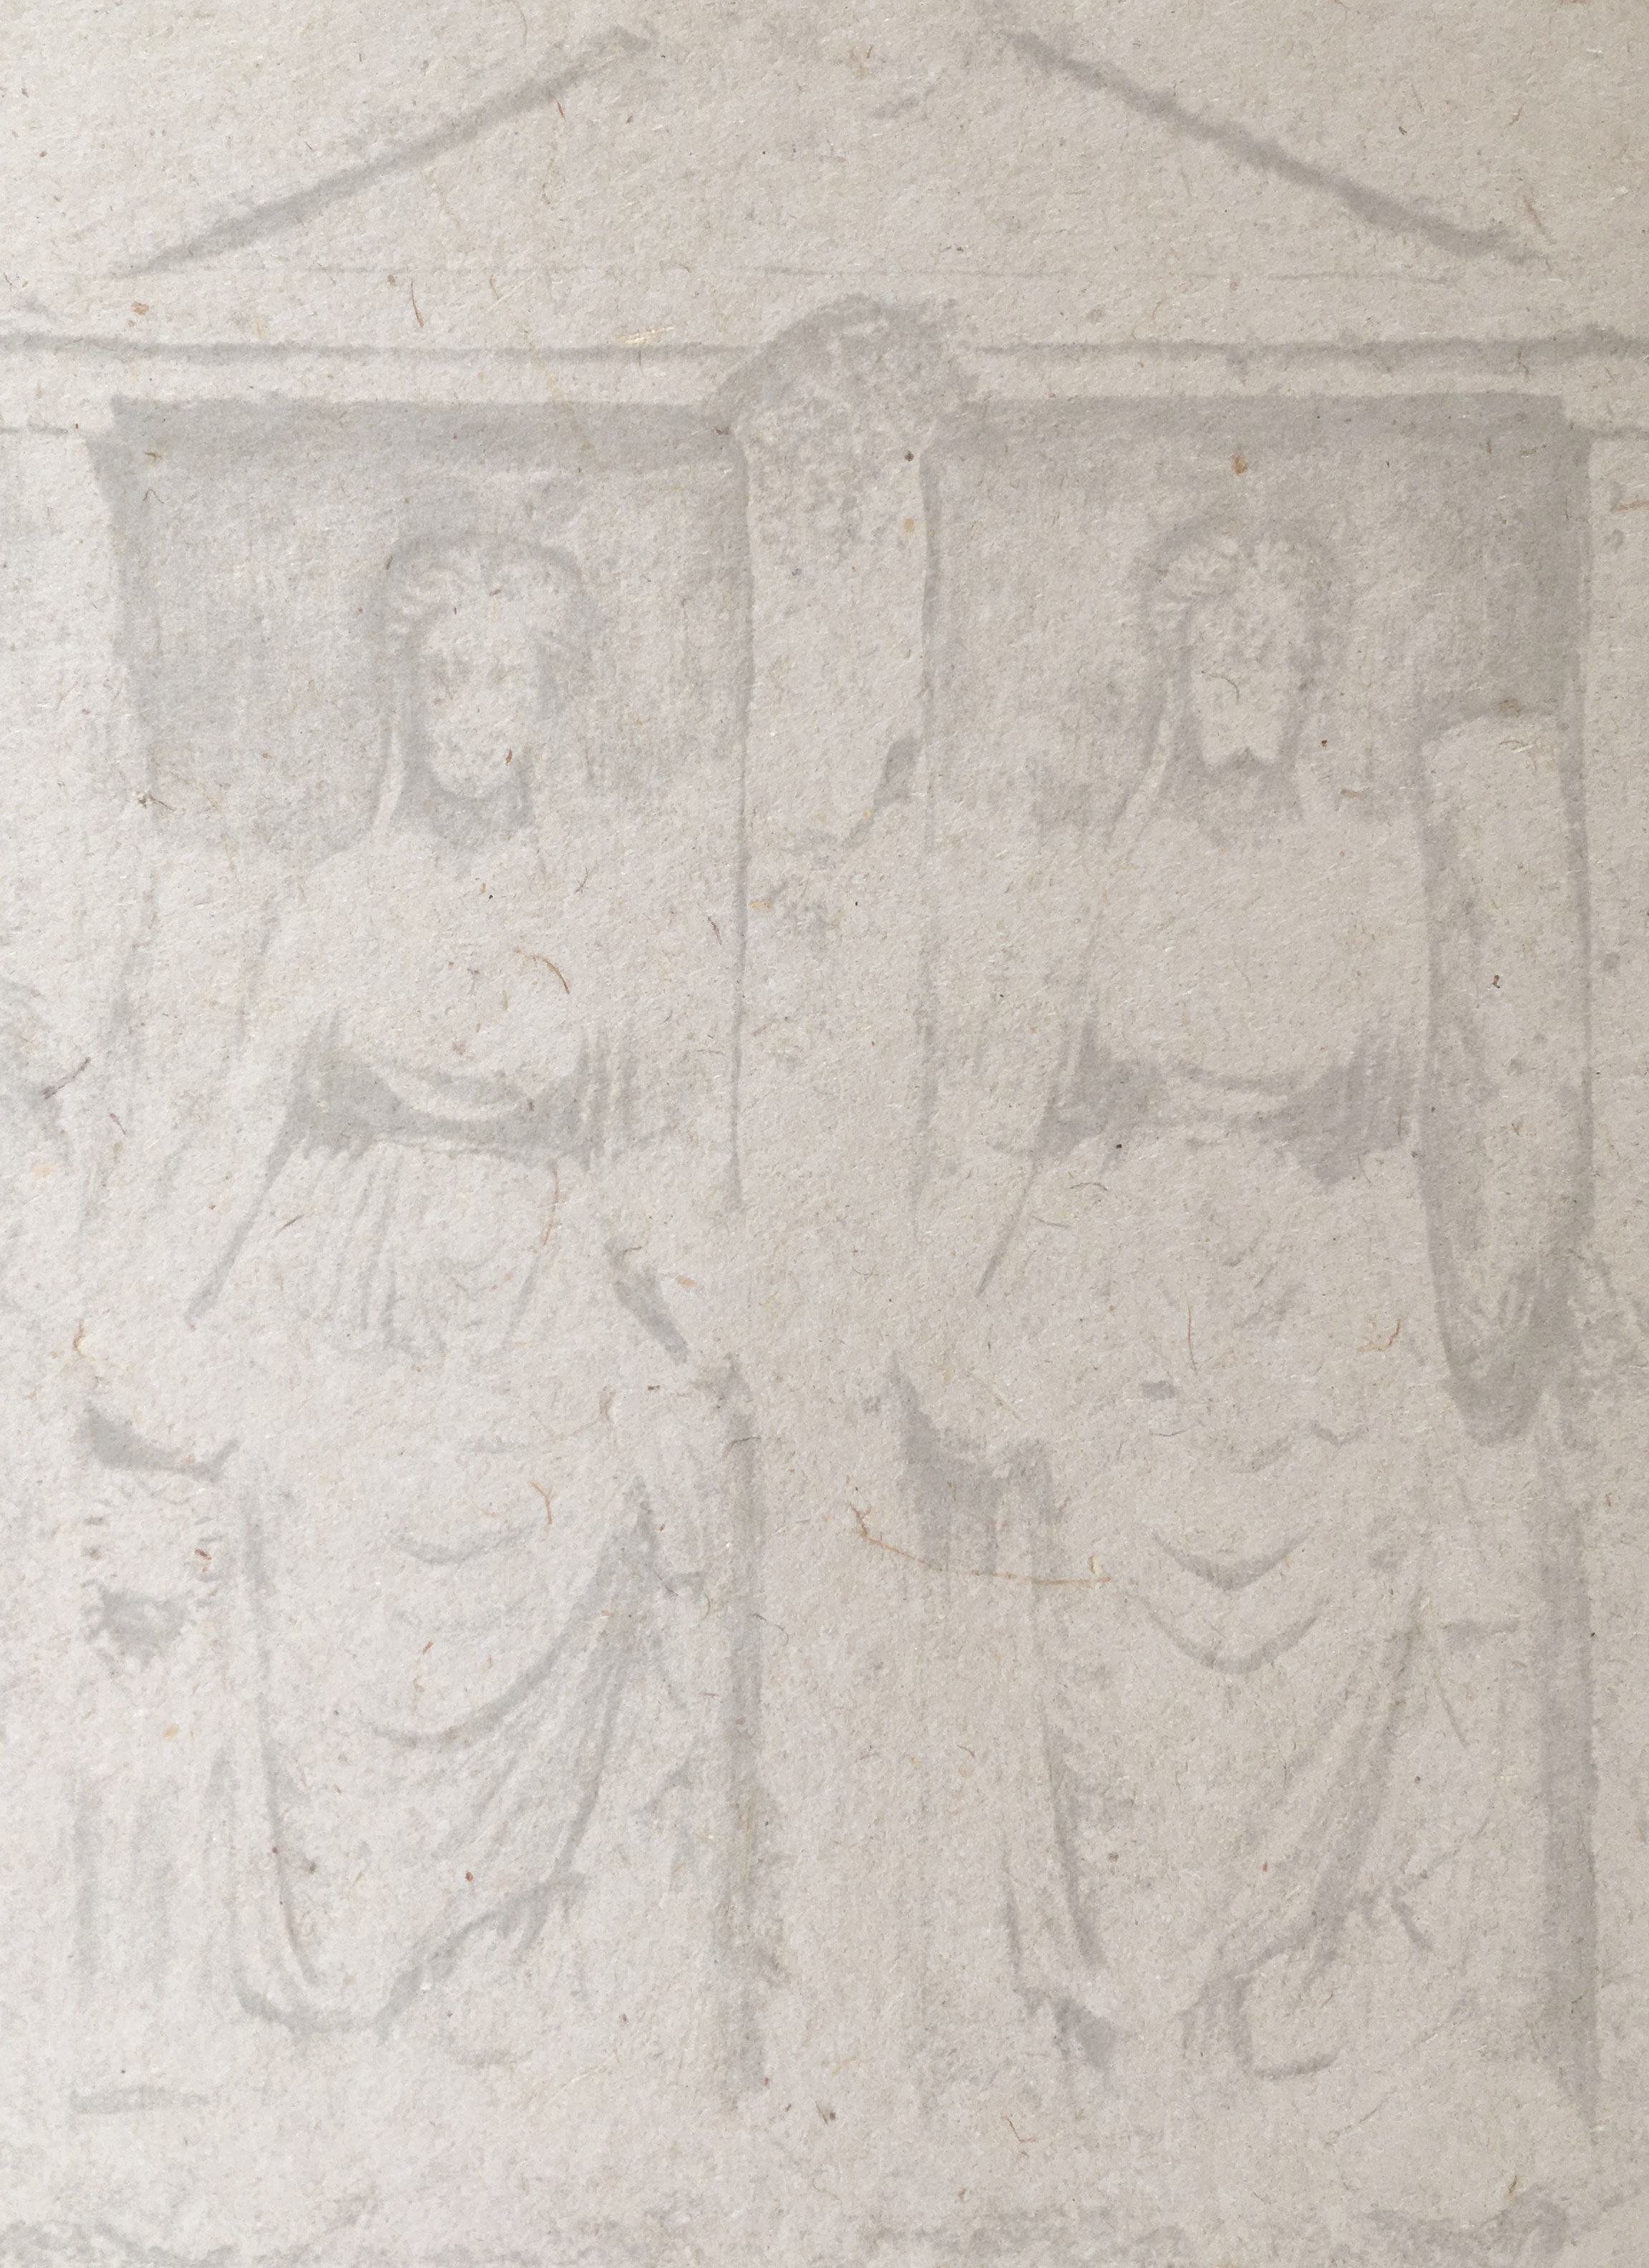
\includegraphics[width=\paperwidth,height=\paperheight]{Hemp_paper_in_Japan8.jpeg}}
\begin{titlepage} % Suppresses headers and footers on the title page
	\centering % Centre everything on the title page
	\scshape % Use small caps for all text on the title page

	%------------------------------------------------
	%	Title
	%------------------------------------------------
	
	\rule{\textwidth}{1.6pt}\vspace*{-\baselineskip}\vspace*{2pt} % Thick horizontal rule
	\rule{\textwidth}{0.4pt} % Thin horizontal rule
	
	\vspace{0.75\baselineskip} % Whitespace above the title

        {\LARGE The Great Mother of the Gods \\} % Title
	
	\vspace{0.75\baselineskip} % Whitespace below the title
	
	\rule{\textwidth}{0.4pt}\vspace*{-\baselineskip}\vspace{3.2pt} % Thin horizontal rule
	\rule{\textwidth}{1.6pt} % Thick horizontal rule
	
	\vspace{1\baselineskip} % Whitespace after the title block
	
	%------------------------------------------------
	%	Subtitle
	%------------------------------------------------
	
	{By \scshape\Large Grant Showerman\\} % Subtitle or further description
	
	\vspace*{1\baselineskip} % Whitespace under the subtitle
	
	%------------------------------------------------
	%	Editor(s)
	%------------------------------------------------
	
	\vspace{1\baselineskip} % Whitespace before the editors

        {\small A Thesis submitted for the Degree of Doctor of Philosophy, University of Wisconsin}

    %------------------------------------------------
	%	Cover photo
	%------------------------------------------------
	
	%\includegraphics[scale=1]{cover}
	
	%------------------------------------------------
	%	Publisher
	%------------------------------------------------
		
	\vspace*{\fill}% Whitespace under the publisher logo
	
	May 1901  % Publication year
	
	{\small Madison, Wisconsin } % Publisher

	\vspace{1\baselineskip} % Whitespace under the publisher logo

        Internet Archive Online Edition  % Publication year
	
	{\small Attribution NonCommercial ShareAlike 4.0 International } % Publisher
\end{titlepage}
\clearpage
\setlength{\parskip}{1mm plus1mm minus1mm}
\tableofcontents
\clearpage
\begin{figure}[H]
\centering
\includegraphics[width=0.80\textwidth,keepaspectratio]{greatmother-1.png}
\caption{Plate 1. --- The Great Mother of the Gods. Statue discovered at Formiæ, now at Copenhagen. (After Lanciani.)}
\end{figure}
\clearpage
\twocolumn
\section{The Introduction of the Cult of the Great Mother at Rome.}
\paragraph{}
The introduction of the Sibylline Books during the reign of Lucius Tarquinius Superbus\footnote{Dionys. Hal. 4 62; Aul. Gell. 1 19. Tarquinius Priscus is sometimes given: Varro in Lact. 1 6, 10; Lyd. \emph{De Mens.} 4 34.} is significant in the history of Rome as marking the point at which the native religion began to be arrested in its natural development and to be transformed under the influence of the religions of the East. It is true that the presence of the Greeks in Italy and the West, through a trade which was considerable, had had its effects on the Roman commonwealth even before this. The Servian constitution bears the marks of the Greek system;\footnote{Mommsen \emph{Hist. of Rome, translated by W. P. Dickson}, 1 123.} the system of weights and measures of the Romans had been brought into relation with that of the Sicilian Greeks;\footnote{\emph{Ibid.} 266.} the Greek alphabet had been communicated through intercourse with Cumae;\footnote{\emph{Ibid.} and Marquardt \emph{Römische Staatsverwaltung} 3 38.} the statue of the Aventine Diana of the Latin confederation had been formed after the image of the Artemis of Ephesus at Massilia.\footnote{Strabo 4 180.} But the intercourse between the Romans and the Italian and Sicilian Greeks was purely commercial, and though its effects are not difficult to see in the less conservative departments of Roman life, in all that pertained to the inner and deeper life of the commonwealth Greek influence was still operating from a distance. Pliny refers the making of the first statue of the gods to the time of Tarquinius Priscus, and Varro says that none existed up to the time of Servius Tullius.\footnote{\emph{N. H.} 35 157; Varro in Aug. \emph{De iv. Dei} 4 31.} So far was the Roman worshiper from investing divinity with human form and human attributes, as the Greek did, that for nearly two centuries the symbolism of a flint for Jupiter,\footnote{Serv. \emph{Ad Aen.} 8 641.} or a lance for Mars,\footnote{Plut. \emph{Rom.} 29.} or a fire for Vesta\footnote{\emph{Ibid.} \emph{Cam.} 20.} was the highest flight his imagination took, while the host of other deities --- and they were as numerous as the acts and duties of the worshiper's life --- remained entirely abstract and formless. The acquisition of the Sibylline Books, then, occurred at a time when Rome had practically no acquaintance with the religions of the East; and the event may be regarded as the first pronounced step in the process which finally resulted in the denationalization of the old-Roman religion and the enthronement of a \emph{turba deorum} whose worship was not in harmony with the genius of the early Romans, and which came to be in harmony with the genius of the later Romans only by reason of the change which that genius gradually underwent. The introduction of the Books is to be regarded primarily as a manifestation in the development of a new religious system; as a cause it is to be regarded only in so far as it facilitated that development in a peculiar manner.

The Books came to Rome from Cumae, and to Cumae they had come from Erythrae, whither they had been brought from Gergis, near Mt. Ida.\footnote{Marq. 3 353.} The fact of their having come from the neighborhood of Mt. Ida is not unimportant; for, consulted as they were ``when insurrection had arisen, or some great calamity in war had befallen the city, or great marvels and visions hard to understand had occurred,''\footnote{Dionys. 4 62.} it often happened that the remedy they prescribed was the introduction of a new cult; and the Books were uniformly partial to those cults which were well known on or near Mt. Ida, their old home.

First among foreign divinities to be introduced through the Sibylline Books was Apollo, who, though the first temple to him was not dedicated until 431 \textsc{B.C.}, became known simultaneously with the introduction of the Books.\footnote{For divinities introduced by the Sibylline Books see Marq. 3 358 sqq.} The institution of the \emph{ludi Apollinares} in 212 \textsc{B.C.} was also due to the same influence. Mercury, to whom a temple was. dedicated in 495 \textsc{B.C.}, followed. In 493 a temple was dedicated to Ceres in connection with Dionysus and Kora, who were identified with the Liber and Libera of the \emph{indigitamenta}, and the \emph{ludi Cereris} were instituted. Proserpina also, not known in the \emph{indigitamenta} as having any connection with the lower world, became identified with Persephone. In the \emph{lectisternium} of 399 \textsc{B.C.}, the first in the history of Rome, and ordered by the Books, the participants were Apollo, Latona, Diana, Hercules, Mercury, and Neptune, showing that Latona had been introduced, that Greek Poseidon was worshiped as Neptune, and that Diana and Hercules were identified with Artemis and Heracles. \emph{Dispater}, to whom and Proserpina the altar in the Terentos was consecrated, is another divinity introduced through the Books, which also caused the \emph{ludi saeculares} to be instituted. In 293 \textsc{B.C.}, in consequence of a plague raging among the people, the Books were again consulted, and gave direction to call to Rome the god Aesculapius, and that divinity was established two years later in a temple on the island in the Tiber. He had been worshiped at Rome before this, but outside the \emph{pomerium},\footnote{Plin. \emph{N. H.} 29 16.} where foreign cults were regularly assigned places unless there was special reason for making them completely national. The \emph{Floralia}, whose character was entirely out of accord with the genius of the old Roman religion, were instituted in obedience to the Books in 238 \textsc{B.C.}, and mark the metamorphosis of the native Flora. Juventas, the Greek Hebe, had a \emph{lectisternium} in 218 by direction of the same authority; and Aphrodite appeared first in Roman affairs in 217, when, by recommendation of the Books, a temple was vowed to Venus Erycina. In the \emph{lectisternium} of the same year, also ordered by the Books, were six \emph{pulvinaria}, with the following divinities: Jupiter and Juno, Neptune and Minerva, Mars and Venus, Apollo and Diana, Vulcan and Vesta, Mercury and Ceres\footnote{Livy 22 10, 9.} --- a system of twelve corresponding to the Greek system. What with the identification of old Roman divinities with strange gods from abroad, and the introduction of other cults entirely new, Rome had taken to herself all of importance that the Greek system offered. Her next acquisition was of necessity to be made elsewhere.

The \emph{lectisternium} of 217 \textsc{B.C.} was held at a time not far removed from the disaster at Trasimenus. The following year was marked by the still more alarming defeat at Cannae. In 215 the death of Hiero of Syracuse deprived Rome of a faithful ally, and in the person of his successor gave the Carthaginian a friend. Tarentum fell in 213, and the list of disasters was interrupted only by the taking of Syracuse by Marcellus in 212. The current now turned, and the capture of Capua in 211, the recapture of Tarentum in 209, and above all the battle of the Metaurus in 207 made it clear that the Roman cause was not lost. But the war had lasted nearly twelve years and had been thoroughly exhausting to Rome. The coinage had been debased; rich and poor had for years been called upon to make sacrifices for the support of the army; payment in all departments was in arrears; fields lay waste even outside the actual theatre of war; prices had risen to thrice their wonted height; and Latium itself, before the Metaurus, had begun to waver.\footnote{Mommsen 2 343.} The victory over Hasdrubal brought a tumult of rejoicing, but when this had subsided, the task confronting the wearied people hardly seemed smaller than before. The invincible Hannibal was still in Italy, and there was need of no less energy now that the war was to be offensive rather than defensive. It was a time when a recommendation of the Books was sure to meet with prompt obedience; and their intervention resulted in the introduction of a cult the history of which from its earliest inception in the East to its fall before Christianity in the fourth century \textsc{A.D.} it is purposed to trace in the following pages.

The consuls for the year 205 \textsc{B.C.}, the fourteenth of the war, were Publius Cornelius Scipio and Publius Licinius Crassus. Scipio was fresh from his command in Spain and was urgent for an African expedition, but met with opposition from the conservative party in the Senate. While the debate was still undecided, the decemvirs, consulting the Sibylline Books on account of the very frequent showers of stones that year, came upon a carmen which said that whenever an enemy from an alien land should wage war on Italy he could be expelled thence and conquered if the Idaean Mother should be brought to Rome from Pessinus. Simultaneously with the report of the decemvirs to the Senate came the report of a legation which had made a pilgrimage with gifts to Delphi. The entrails had been auspicious, and a voice had come from the shrine telling them that the Roman people were about to win a victory far greater than that from the spoils of which (probably Metaurus) the legates bore gifts. This coincidence, together with the thought of Scipio, who had demanded Africa as his province as though his soul were prescient of the end of the war, decided the course of the Senate. The Romans at that time had no allies in Asia, but the friendship of Attalus of Pergamum had been secured in the war which they had aided him to carry on against Philip, and they looked to him for aid in effecting the transfer of the goddess. An embassy of five citizens of note was selected, and five quinquiremes had voted them. Visiting Delphi on their way, they were assured that they would receive aid from Attalus, and were also directed to provide for the reception of the goddess in behalf of the State by the ``best'' man at Rome. Arrived at Pergamum, the king received them cordially, conducted them to Pessinus, and handed over to them the sacred stone --- \emph{lapis quidam non magnus, ferri manu hominis sine ulla impressione qui posset, coloris furvi atque atri, angellis prominentibus inaequalis}\footnote{Arnob. \emph{Adv. Nat.} 7 49.} --- which the natives of the place said was the Mother of the Gods.\footnote{Varro \emph{L. L.} 6 15 gives Pergamum as the city whence the image was brought. Cf. Ovid \emph{Fast.} 4 265 sq. This view, however, is not shared by other authorities, and Pessinus is thought of throughout the history of the cult as the ancient seat of the image.} The object of their mission attained, the legates sent one of their number in advance to report the fact to the Senate and to communicate the will of the oracle in regard to the reception of the divinity. Publius Scipio Nasica, the son of the Gnaeus Scipio who had fallen in Spain, a youth not yet arrived at the quaestorial age, was selected as the best man in the State, and commissioned to meet the goddess at Ostia. The day of the arrival was made a holiday; the foremost matrons of Rome, among them Claudia Quinta, whose reputation had suffered from slander, but whose fame became more brilliant after the ministry of that day, received the goddess from Scipio's hands; and as by turns they carried her to the city the whole commonwealth thronged to meet them, censers were placed before the doors wherever they passed, incense was burned, and prayers were offered that propitiously and with good will the goddess would enter the city. Arrived at Rome, she was borne to the temple of Victory on the Palatine, inside the \emph{pomerium}, contrary to the usual practice on the introduction of foreign divinities. The date was the day before the Nones of April, 204 \textsc{B.C.} The people in great numbers brought gifts, there was a \emph{lectisternium}, and games called \emph{Megalensia}.\footnote{Livy 29 10-14.}

This is the historian's account, and is an attempt to give a faithful picture of the first scene in the history of the cult at Rome. The Mother appears as a dignified Roman deity. The account of the poet differs in that it introduces the marvelous and invests the scene with the attributes of the worship as it was in the time of its full development in the East.\footnote{Ovid \emph{Fast.} 4 178 sqq.} According to the poet's version, the coming of the Mother is the final act in the Trojan emigration; she had wished to come with Aeneas, but the fates had decreed otherwise, and she had remained content with giving him her trees for his ships.\footnote{Verg. \emph{Aen.} 9 80 sqq.} Attains is not willing to grant the Romans their desire; they plead their kinship with Aeneas, and his coming to Rome;\footnote{Herodian 1 11, 3.} the earth trembles and rumbles, and the goddess herself speaks:
\begin{quote}
Ipsa peti volui. Ne sit mora. Mitte volentem.\\ Dignus Roma locus quo deus omnis eat.\footnote{Ovid. \emph{Fast.} 4 267-270.}  
\end{quote}
\paragraph{}
After her long journey by sea along the storied coasts of the Mediterranean, she finds assembled to meet her at the Tiber's mouth the knights, senators, and common people, with mothers, daughters, and Vestals in the front. The ship is drawn into the mouth of the stream by cables, but in vain are the efforts to move it far; the water is low, and the ship becomes fast in the marshy shallow. Confusion seizes the multitude at the omen; the ship is as firm as an island. Claudia Quinta, of noble birth and as beautiful as she is noble, chaste but not untouched by slander, steps forth from the line of mothers, daughters, and Vestals,\footnote{Julian Imp. \emph{Or.} 5 160 and Aurel. Vict. \emph{De Viris Illust.} 46 call Claudia a Vestal, confusing her with Claudia Vestalis, daughter of Appius Claudius Pulcher, Consul 143 \textsc{B.C.} Herodian 1 11 mentions a Vestal as performing the miracle, but gives no name. Others are consistent in giving her merely as Claudia Quinta. Lact. 2 7, 12, says of her: \emph{impudica esset habita ob nimios corporis cultus}; and Appian \emph{Hann.} 56 tells us that she was charged with adultery, but not yet judged.} dips her hands into the waters of the Tiber, sprinkles thrice her head, lifts thrice her palms to the heavens, kneels to the goddess, strong in the consciousness of her own purity, and with hair no wing loose, calls upon her for vindication from the charges of her enemies. Then rising, with only slight exertion she draws the sacred craft up the stream, while the multitude sends cries of joy to the skies.

But night falls before they have reached Rome, and they halt at a bend of the river. The following morning they burn incense, sacrifice a heifer before the garlanded stern, and continue the journey. Arrived at the Almo, a small stream which flows into the Tiber not far south of Rome, a hoary priest clad in shining vestments laves the goddess and the sacred utensils in its waters, while his attendants utter wild cries to the frenzied music of flutes and the beating of the tympanum. Claudia precedes the multitude, and the goddess herself, in a chariot drawn by oxen bedecked with fresh flowers, is borne through the Porta Capena, where Scipio receives her.
\clearpage
\onecolumn
\begin{figure}[H]
\centering
\includegraphics[width=0.95\textwidth,keepaspectratio]{greatmother-2.png}
\caption{The Miracle of Claudia. Relief in the Capitoline Museum. (After Baumeister.)}
\end{figure}
\clearpage
\twocolumn
\section{The Great Mother in the East}
\paragraph{}
The original home of the goddess who thus auspiciously took up her abode on western soil was within the limits of Asia Minor. It is true that among the Greeks, who saw in the Asiatic Mother their own Rhea, the ill-treated mother of Zeus, the idea was not uncommon that the latter had but transferred her seat from Crete to the more congenial wilds of Asia Minor;\footnote{\emph{Scholia Victoriana ad Iliad.} 24 675: ἐν Σιπύλῳ, ὅθι φασὶ θεαων ἔμμεναι εὔνας, \emph{sic tradunt}. Ῥέα γὰρ φοβηθεῖσα τὰς ἀπειλὰς Κρόνου, σὺν ταῖς θυγατρασι ὤκησε Σίπυλον κρυφίῶς ίερον ἀυτῷ (αὐτῇ) ἐκεὶ. Cf. \emph{Orac. Sibyll.} 5 130, 1.} but Demetrius of Scepsis, about 190 \textsc{B.C.}, expressly denies that the worship of Rhea (meaning the Phrygian Great Mother) was either observed in or native to Crete, and says that it belonged only to Phrygia and the Troad, and that those who asserted the contrary recited legend rather than fact. The homonymy of places is a cause of the confusion, he says; for there is a Trojan Mt. Ida and a Cretan Mt. Ida, \emph{etc., etc.}\footnote{Strabo 472.} But if there were those who, through confusion of the Asiatic Mother with Rhea, believed her to have come from Crete, the origin and growth of her worship is unanimously located in Asia Minor, in the central, western, or northwestern portions. Neanthes of Cyzicus attributed the founding of the cult in his city to the Argonauts,\footnote{\emph{Ibid.} 45. Cf. Apollonius Rhodius \emph{Arg.} 1 1078-1152.} and Herodotus represents the Cyzicenes as holding an annual festival in honor of the Mother of the Gods in the sixth century.\footnote{4 76.} There was also a temple at Sardis, where the cult was of such long standing that the divinity was called by Herodotus ἐπιχωρίη;\footnote{5 102.} and the various legends agree in locating the rise of the worship in Galatia, Phrygia, Lydia, or on the borderland between.\footnote{Diod. Sic. 3 58; Paus. 7 17; Arnob. 5 5; Firm. Mat. \emph{De Error.} 3; Ovid \emph{Fast.} 4 223 sqq.; Sallust. Phil. \emph{De Diis et Mundo} 4; Jul. \emph{Or.} 5 165 sqq.}

Notwithstanding the almost universal designation of the Mother as Phrygian in later times, she was not of Phrygian origin ethnographically. Ramsay has pointed out that the social and religious system of the Phrygian race, which invaded Asia Minor from the North about 900 \textsc{B.C.}, was patriarchal, while the system of the native race which they conquered was matriarchal.\footnote{\emph{Jour. Hell. Stud.} 9 367.} It is therefore probable that the Phrygians, on their entrance into the interior of the peninsula, found a deity whom the native inhabitants worshiped as a Great Mother, and that the later Phrygian Great Mother was only a development of that divinity.

The Great Mother, then, was really pre-Phrygian in origin, and can be called Phrygian only in a geographical sense. As late even as the transfer of the image to Rome she was not yet generally regarded as Phrygian. Apollonius Rhodius calls her ἐνναέτης Φρυγίης,\footnote{\emph{Arg.} 1 1126.} but the cult had its strongest center in Pessinus in Galatia, a city beyond the borders of Phrygia, which received its name, according to one legend, from having been the spot where the sacred stone fell (πεσεῐν) from heaven.\footnote{Herodian 1 11: ἐκ τοῦ πεσοντος ἀγαλματος ἐξ ουρανοι.} Sophocles knows the Mother as the great goddess who rules by the Pactolus, a stream near Pessinus;\footnote{\emph{Phil.} 390.} Pausanias and Arnobius, quoting early legends, call her Ἄγδιστις, from a mountain which the former calls Agdistis and locates near Pessinus, and which the latter calls Agdus;\footnote{Cf. note 29.} an epigram in the Palatine Anthology designates her as ἢ παρὰ Σαγγαρίῳ Μάτηρ, the Sangarius being another stream near the city.\footnote{6 234.} Other centers of her worship, less famous, were Cyzicus, where she was called Δινδυμία and Λοβρίνη, from the neighboring mountains Dindymon and Lobrinon;\footnote{Apollon. \emph{Arg.} 1 1125; Nicand. \emph{Alex.} 8 and scholia.} the neighborhood of still another Mt. Dindymon, between Lydia and Phrygia, where Herodotus knew her as Δινδυμήνη;\footnote{1 80.} and Mt. Ida in the Troad, where she was called Μήτηρ Ἰδαία.\footnote{Eurip. \emph{Orest.} 1453; Apollon. \emph{Arg.} 1 1128. There are numerous other designations derived from places of worship at a later time which will be cited in their proper place. To secure continuity and to avoid investing the purely Asiatic Mother with Greek or Roman characteristics, as sparing use as possible is made in this chapter of testimony not antedating the Roman visit to Pessinus, both as to names, character, and details of worship.}

The name by which the Great Mother became commonly known to the Romans and which is the usual modern designation, Κυβέλη, \emph{Cybele}, occurs first on an altar near Prymnessus, inscribed \emph{Matar Kubile}.\footnote{Ramsay \emph{Jour Hell. Stud.} 3 35-41; 5 244-246.} It is essentially a literary name, however, and is extremely rare in inscriptions. It makes its first appearance in literature in Pindar.\footnote{\emph{Frag.} 80 Bergk. It is foreshadowed, however, by the use in Hipponax, \emph{frag.} 121 Bergk, of Κὑβηλις, an adjective form.} Aristophanes and Euripides use it, and it was so well known by the time of Strabo that he gave his version of its derivation. According to him, it is to be derived, like so many other designations of the Mother, ἀπὸ τῶν τόπων, κατὰ τοὺς τόπους, and the τόπος from which this one was taken is a mountain or range of mountains.\footnote{469; 470; 567: καθάπερ ἀπὸ τῶν Κυβέλων ἡ Κυβέλη.} Diodorus derives it from a mountain Κύβελον.\footnote{3 58.} Stephanus of Byzantium, s. v. Κυβέλεια, calls Κύβελα a sacred mountain, from which Κυβέλη ἡ Ῥέα is called Κυβεληγενής and Κυβελίς; and Hesychius and Suidas, understanding a range rather than a single peak, explain it as ὄρη Φρυγίας.\footnote{Κυβελα' ὄρη Φρυγίας καὶ ἄντρα καὶ θάλαμοι. Of. schol. to Aristoph. \emph{Birds} 877. Another derivation is from a city Κυβέλλα. Hipponax \emph{l. c.}: παρὰ τὸ ἐν Κυβέλλᾳ πόλει Φρυγίας τιμᾶσθαι.} The parallel form Κυβήβη, \emph{Cybebe}, which became common among Latin writers, was used as early as the end of the sixth century \textsc{B.C.} by Charon of Lampsacus, quoted by Photius under the word Κύβηβος, with which he considers Κυβήβη to be connected.\footnote{Κύβηβος ὁ κατεχόμενος τῇ μητρὶ τῶν θεῶν, θεοφόρητος Κυβηβᾶν μαίνεσθαι, ἐνθουσιαν. In \emph{Etymol. Mag.} 543, 22 κύβη, the head, is given as the root of κύβηβος, κυβιότάω, \emph{etc.} Martianus Capella 7 740 derives Cybebe from \emph{cubus}, a cube, Gr. Κύβος.} Still another form, Κυβήκη, appears in Hesychius.

Thus far the appellations cited have been almost without exception derived from localities where the cult of the goddess thrived. Among those derived rather from her character the most common is μήτηρ θεῶν.\footnote{Herod. 4 76.} Other designations and epithets in this Class are μάτηρ μεγάλα, πολυπότνια, παμπότνια, μήτηρ συμπάντων μακάρων, μήτηρ πάντων τε θεῶν πάντων τ᾽ ἀνθρώπων, μεγάλη μήτηρ θεῶν καὶ ἀνθρώπων, παμβῶτις, μάτηρ αὐτοῦ Διός, παντότεκνος, μάτηρ ὀβρίμα, ὀρεία, ὀρεστέρα, δαίμων οὐρείη, and ἀνταίη δαίμων.\footnote{Eurip. \emph{Bacch.} 78 and Pindar \emph{Frag.} 57 Bergk; Apollon. \emph{Arg.} 1 1151; \emph{Anth. Pal.} 6 281; Apollon. \emph{Arg.} 1094; \emph{Hom. Hymns} 13; Aristoph. \emph{Birds} 875; Soph. \emph{Phil.} 389; \emph{ibid.}; Kaibel \emph{Epig.} 44; Eurip. \emph{Orest.} 1453; \emph{ibid.} \emph{frag.} 475, 13; Soph. \emph{Phil.} 389; Apollon. \emph{Arg.} 1 1119; \emph{ibid.} 1141; \emph{Orphic Hymns} 30, 5 calls the Mother ὀρειομανής, and Orph. \emph{Arg.} 547 παμμητειρα.}

In a study of the character of the Great Mother and her worship before her cult had spread beyond the limits of Asia Minor, to approximate the truth is all that is possible; for our appreciation of the religion of early Asia Minor depends upon evidence given in the literature, art, and inscriptions of two foreign peoples, and that too given for the most part at a date late enough for the currents of outside influence to have had no small modifying effect. If Greek art, its elements borrowed from the East and perfected on its own soil, could early return and teach its progenitors, it is likely also that Greek religion early influenced that of the interior of Asia Minor. The Great Mother, therefore, cannot be seen in her purely Asiatic aspect. While that part of her nature which is agreeable is the more attractive when viewed in the golden light of Greek poetry, that part which is repulsive is no doubt also seen in an exaggerated form.

The universal motherhood of the goddess is the feature of her character most frequently brought to the attention. She is Mother of the Gods, Great Mother, Mistress of All, Mother of All the Blest, Mother of All Gods and All Men, All-nourisher, All-begetter. She is Mother of Zeus himself. ``The winds, the sea, the earth, and the snowy seat of Olympus are hers, and when from her mountains she ascends into the great heavens, the son of Kronos himself gives way before her, and in like manner do also the other immortal blest honor the dread goddess.''\footnote{Apollon. \emph{Arg.} 1 1098 sqq.}

She is thus the great parent of all nature. As Phrygia and its neighborhood, though a mountainous region, has also its rich, fertile valleys, she is as well a guardian over man and his interests in the form of flock and herd and growing vegetation as over the untamed and uncultivated parts of the natural kingdom. But it is her character as a deity of wild nature that comes most prominently to view. She is the Mountain Mother, the Mighty Mother of Ida, the Divinity of the Mountains. She has a passion for the mountains, almost invariably has her sanctuaries on the mountains, and frequently takes her name from them. Her usual designation Κυβέλη is derived either from mountains or caves. She has places of worship in caves; Nicander mentions Ῥείης Λοβρίνης θαλάμαι, which are explained as τόποι ἱεροὶ ὑπόγειοι.\footnote{\emph{Alex.} 8 and schol.} She has dominion over the sea and the winds; when the Argonauts founded her cult at Cyzicus, the halcyon was her messenger, and in her name foretold a calm. An altar of stones was reared to her there on the mountain, and the Argonauts made sacrifice garlanded with the leaves of the oak, which was sacred to her, while her image was fashioned from a vine.\footnote{Apollon. \emph{Arg.} 1084-1124 and schol.} The poet of \emph{Hom. Hymns} 14 addresses her as one who delights in the clamor of wolves and gleaming-eyed lions, in echoing mountains and woodland haunts. Anacharsis the Scythian worships her in a place πλέῃ δένδρων.\footnote{Herod. 4 76.} She is Φρυγίων θρέπτειρα λεόντων, and lions are her faithful companions in literature and art throughout her history.\footnote{\emph{Anth. Pal.} 6 51; see below, p. 317.} She is λεοντόδιφρος, and ταυροκτόνων λεόντων ἔφεδρος.\footnote{\emph{Anth. Pal.} 6 94; Soph. \emph{Phil.} 395.} In the Phrygian legend given by Diodorus she cares for men and flocks, and there is a suggestion of the witch in her healing children by magic.\footnote{3 58.} She herself as a child is exposed on the mountains, is nourished by wild beasts, and is associated with the satyr Marsyas in her mad wanderings. In \emph{Anth. Pal.} 6 281 she is called on to hasten the maturity of the little Aristodice for the duties of wedlock. Finally, her universal power over the natural kingdom is nowhere more charmingly described than in Apollon. \emph{Arg.} 1 1140 sqq.: The trees showered down fruit in wondrous wise, and at their feet of her own accord did the earth send forth the blossoms of delicate herbage. And wild creatures, leaving their dens and the thickets, came forth fawning. And yet another wonder did she perform; for never before had Dindymon streamed with water, but at that moment did it jet forth before them unceasingly from the parched ridge.

Still more evidence as to the essential wildness of the Great Mother's character is found in the nature of her priests and their manner of worship. The mythical Idaean Dactyloi were the first to discover and forge iron, and had learned the art from their mistress, the Great Mother.\footnote{Strabo 473; schol. to Apollon. \emph{Arg.} 1 1129.} Her mythical attendants, the Corybantes, early became a synonym for what was noisy and orgiastic.\footnote{Eurip. \emph{Bacch.} 125.} The Curetes, whose din of spear and shield at the birth of Zeus had drowned the infant's cries and saved him from Kronos, also became servants of the Mother upon her confusion with Rhea.\footnote{In \emph{Orph. Hymns} 30 they are so represented, and are called σκιρτηταί leapers, ποσσίκροτοι, beaters of the foot in the dance, ῥομβηταί, whirlers, ὀρέστεροι, creatures of the mountains, ὀργιοφάνται, teachers of orgies, \emph{etc.} --- designations which, of course, describe also the priests of the Mother at that time.} The actual priests of the goddess were called Γάλλοι, a name which the ancients explained as taken from the stream Gallus, which flowed into the Sangarius not far from Pessinus,\footnote{Plin. \emph{N. H.} 5 147, 6 4; Herodian 1 11. Movers \emph{Die Phoenizier} 687 derives it from a Semitic root, and gives it a meaning similar to that of Corybas, \emph{Kopfschüttler}, and κυβηβος. Stephanus s. v. \emph{Gallus} relates that a Phrygian priest of that name in the service of the Mother, after having castrated himself in a frenzy, lay down by a stream, which was known thereafter as the Gallus.} and on the banks of which the orgies of the Mother took place. The waters of the stream were fabled to inspire madness in those who drank of them.\footnote{Ovid \emph{Fast.} 4 365.} The name Galloi first appears in the beginning of the second century \textsc{B.C.}, in the Alexandrian epigrams of the \emph{Anthologia Palatina}. The priests were further called γόητες, sorcerers, θαλαμηπόλοι, dwellers in chambers (caves?) ἀμφίπολοι θαλάμης.\footnote{\emph{Anth. Pal.} 6 173, 220; 9 340.} They were eunuchs, were attired in female garb, and wore their hair, fragrant with ointment, wound in coils on the top of the head, letting it hang loose, however, while performing their orgies. Priests, and priestesses, who were as common as priests in the service of the Mother, often dedicated to the goddess their locks, which they had tossed wildly in the frenzied dance.\footnote{\emph{Ibid.} 6 217-220.} The attempt to derive Cybebe from κύβη, the head, has been noted. Clothing and instruments, as well as hair, were sometimes dedicated.\footnote{\emph{Ibid.} 6 51, 234, 237.} Anacharsis the Scythian, attempting to introduce the worship among his countrymen, sacrificed ἐκδησάμενος ἀγάλματα.\footnote{Herod. 4 76.}

The instruments used in the worship were no less in accord with the wild nature of the Mother. There was the αὐλός, flute, whose invention is credited to the goddess herself.\footnote{Diod. 3 58. Hyagnis is the inventor in \emph{Anth. Pal.} 9 340 and \emph{Marm. Par.} 10.} The κρόταλα were hand-clappers, or castanets, used in the dance.\footnote{\emph{Anth. Pal.} 7 223. Suidas describes them as σχιζόμενος καλαμος. Publilius Syrus calls the stork \emph{crotalistria}, and a chatterbox in \emph{The Clouds} is called κροταλον.} Thirdly, there were the κύμβαλα, cymbals, brazen disks, hollowed and sharp-toned --- ὀξύδουπα κοιλοχείλεα.\footnote{\emph{Anth. Pal.} 6 94.} Most frequently mentioned of all is the τύμπανον, τύπανον, tympanum, described by Photius as ἐκ δερμάτων γινόμενον καὶ κρουόμενον ὅ κατεῖχον αἱ Βάκχαι. It was also described as βυρσότονον κύκλωμα, and was native to Phrygia.\footnote{Eurip. \emph{Bacch.} 58, 124. The Mother is τυμπανοτερπης in \emph{Orph. Hymns} 26, 11.} It was a necessary part of the equipment of a priest in the sixth century,\footnote{Herod. 4 76.} and Euripides calls it the invention of Dionysus and Rhea (Cybele), and of the Corybantes.\footnote{Eurip. \emph{l. c.}} In \emph{Anth. Pal.} the story is repeated several times of a Gallus who met a lion in a cave, frightened the savage beast by sounding his tympanum, and afterwards dedicated the instrument to the goddess.\footnote{6 217, 218, 219.} Diogenes Tragicus mentions mitre-wearing women of Asiatic Cybele, daughters of wealthy Phrygians, with tympana, rhomboi, and the clashing of brazen cymbals.\footnote{Athen. 636.} The rhombus mentioned here was an instrument of the drum or tympanum kind, but does not seem to have been common, at least in later times.\footnote{Apollon. \emph{Arg.} 1 1139; cf. ῥόπτρον, \emph{Anth. Pal.} 6 74.} In Pindar appears also the torch --- αἰθομένα δᾷς ὑπὸ ξανθαῖσι πεύκαις --- indicating night celebrations, which may have been, however, a Greek addition.\footnote{Frag. 57 B; cf. Herod. 4 76; \emph{Anth. Pal.} 6 173; 7 223.} All the instruments of the cult are classed as οἰστρήματα λύσσης, and served to inflame the ministers and worshipers of the goddess to the highest pitch of enthusiasm. Mad yelling was another feature of the worship. Nicander compares the shrieks of a madman to the curdling yell --- ῥιγηλὸν ὑλαγμόν --- of a priestess of the Mother, which makes all shudder who hear.\footnote{\emph{Alex.} 217-220.} A Gallus in the Palatine Anthology is μάκρ᾽ ὀλολυζόμενος.\footnote{6 234.} A place of worship is called ὀργαστήριον.\footnote{Nicand. \emph{Alex.} 8.} The frenzied excitement of priests is μανία and λύσσα, and its culmination is self-scourging, or self-laceration with knives, to symbolize the supreme act of consecration to the Mother, which consisted in self-emasculation. The eunuch Alexis, after the ecstasy of the orgies, dedicates his sharp-voiced cymbals, his deep-toned flutes, made of the horns of a calf, his sonorous tympana, his yellow locks, tossed in the dance, and his knives, stained with red blood.\footnote{\emph{Anth. Pal.} 6 51.} Epithets applied to the Galloi in token of their emasculation and chastity are θῆλυς, κειράμενος γονίμην, ἴθρις, ἄγνος, νεήτομος, Γάλλαι.\footnote{\emph{Ibid.} 6 51, 218, 219, 220, 234.} The act by which they deprived themselves of manhood and consecrated themselves to the service of the Mother was voluntary, and sometimes performed by their own hands when they were at the highest point of frenzied excitement.\footnote{Schol. Nicand. \emph{Alex.} 8; Serv. \emph{ad Aen.} 9 115; Catull. 63 4, 5; cf. Plin. \emph{N. H.} 35 165: \emph{Samia testa Matris Deum sacerdotes qui Galli vocantur virilitatem amputare, nec aliter citra perniciem}.} The custom makes its first appearance, together with the Galloi, in Alexandrian literature, about 200 \textsc{B.C.}, and was probably of Semitic origin.\footnote{Rapp, Roscher's Lex. 2 1, 1657.}

A complete account of the rites and festivals of the Great Mother while she was yet purely Asiatic, cannot be given. The Argonauts poured a libation to her over a blazing sacrifice, accompanying the rite with a dance in which they clashed together their shields and swords, from which Apollonius derives the use of the rhombus and the tympanum of his time.\footnote{Apollon. \emph{Arg.} 1 1134-1140.} A priestess in Nicander is called βωμιστρια, altar-attendant, and κερνοφόρος, bearer of the κρατήρ.\footnote{\emph{Alex.} 217.} The Galloi are also called μητραγύρται, begging priests of the Mother, showing the manner in which the cult was supported.\footnote{Antiph. in Athen. 553 C; Dion. Hal. 2 19, 4.} Arrian says that the day of lamentation and the bathing of the Mother were Phrygian customs taken over into the Roman cult,\footnote{\emph{Tact.} 33, 4.} and it is probable that there was a series of festal days every spring in Phrygia as there was at Rome under the Empire, of which the bathing of the goddess in the stream Gallus occupied one day. Servius also states that the Romans worshiped according to the Phrygian manner,\footnote{\emph{Ad Aen.} 12 836.} but it is unsafe to invest the early cult in Asia Minor with all customs practiced centuries afterward among a people so different from the eastern peoples as the Romans were.

Inseparably connected with the Great Mother is the strange being known as Attis. A study of the various versions of the legend in which he appears will serve to give a fuller appreciation of the character of the Mother as well as to show the relation which the two bear to each other. The legend first makes its appearance in the elegiac poet Hermesianax, about 340 \textsc{B.C.} It is given in abstract by Pausanias, and is meant to account only for the origin of Attis. Attis was the son of Calaus, a Phrygian, and was impotent from his birth. Arrived at the age of manhood, he migrated to Lydia, where he instituted the worship of the Great Mother. He was held in so great honor by the Lydians that Zeus in anger sent into their fields a savage boar, which destroyed Attis and also some of the Lydians. But, continues Pausanias, the Phrygians themselves do not believe this story. There is another legend among them, which says that Zeus in his sleep having discharged seed upon the earth, a monster having both male and female organs sprang into existence. Agdistis was the name given the monster, which was of such terror to the gods that they deprived it of male organs, from which in turn sprang an almond tree, from the effect of whose fruit the daughter of the river Sangarius bore a son. The child was exposed; but, having been cared for by a he-goat, it became beautiful surpassing the human, and inspired love in the breast of Agdistis. When this child, who was named Attis, was of suitable age, his kinsmen sent him to Pessinus to espouse the king's daughter; but during the nuptial hymn Agdistis suddenly appeared, whereupon Attis in a frenzy emasculated himself, his example being followed by the king. Agdistis, seeing the consequences of the madness which she had inspired in Attis, repented of her act, and prevailed upon Zeus to grant that the body of the youth should never decay nor waste. These are the best-known legends about Attis, concludes Pausanias.\footnote{7 17, 9-12.} Elsewhere he states that the burial-place of Attis is on the mountain Agdistis at Pessinus.\footnote{1 4, 5.}

Another version, differing only in details, is given by Arnobius, a Christian writer of the fourth century, on the authority of a certain Timotheus, otherwise unknown to us, ``and others equally learned who have drawn their information from recondite works on antiquity.'' The mountain here is called Agdus, instead of Agdistis, and it was in this place that Deucalion and Pyrrha created the human race, among whom was also the Great Mother. Zeus having been disappointed in his love for her, Agdistis comes into being as in the story of Pausanias, and is deprived of male attributes by a stratagem of Dionysus. From the blood springs a pomegranate tree, whose fruit, in the same manner as that of the almond in Pausanias, brings into being a child, called Attis for his beauty. His mother is Nana, the daughter of the river-god Sangarius; she is imprisoned by her father, who intends to starve her, but is nourished by her mother with apples and other food until the child is born. The Mother of the Gods and Agdistis are both enamored of the youth Attis, and the latter gives him in secret many gifts of the chase. Attis finally betrays the secret of their love while in wine. The king and his daughter are both named in this version --- they are Midas and Ia. On the occasion of the marriage, which he has planned in order to rescue Attis from the shameless love of Agdistis, Midas orders the city gates to be closed, but the Mother of the Gods, for the good of the youth, whose fate she knows, raises the walls of the city on her head and enters. Agdistis strikes madness into the entire company, and Attis, exhausted by his frenzy, at length throws himself down under a pine tree, emasculates himself, delivering to Agdistis the mutilated organs with the words: \emph{tibi, Agdesti, haec habe, propter quae motus tantos furialium discriminum concitasti}. But the Mother buries them, and violets spring from them; and as for Ia, having enveloped the body of Attis in wool and mourned over him in company with Agdistis, she kills herself and is buried by the Mother, purple violets springing from her blood and the almond from her grave. The Mother bears the fatal pine into her cave and in company with Agdistis wildly laments the death of Attis. Zeus will not restore him to life, for that is against the will of the Fates, but he consents to allow the body of the youth to remain undecayed, his hair to continue to grow, and his little finger to move, whereupon Agdistis consecrates the body in Pessinus and causes it to be honored annually with priestly ceremonies.\footnote{Arnob. 5 5-8.}

The above accounts are intended by their authors merely to present the origin of Attis, and the mention of the Mother is incidental. There is no need to suppose, with Rapp, that Agdistis and the Mother are identical, and that Arnobius has blended several accounts in ignorance of it.\footnote{Roscher's Lex. 1 1, 716.} The conception of the Great Mother as a monster like Agdistis, which this would imply, nowhere appears, nor does the conception of Attis as in any way a blood descendant of the Mother appear. The appearance of the Mother at the nuptials of Attis and Ia is not, as Rapp asserts, without motive; she is impelled by her love for the youth, and by her knowledge that he is fated to remain safe only as long as he is not bound by marriage ties --- \emph{ne quid accideret maesti}.\footnote{Arnob. 5 7.} Her behavior throughout is that of a protectress-lover, while the character of Agdistis exhibits nothing in common with that of the Mother. It is true that the Mother was occasionally known by the name of Agdistis,\footnote{Strabo 469, 567.} but this points to a confusion of the legend of Attis' birth with the legend of his relations with the Mother, or it is an appellation derived from the rock Agdus, the scene of her creation by Deucalion and Pyrrha. The version of Arnobius is a blending of two tales, but not two tales presenting the same characters. He or his authorities blended, or found already blended by tradition, one legend of the birth of Attis and another legend of the relations of Attis and the Mother.

Still another account, given as Phrygian tradition, is found in Diodorus. In this version the Mother, rather than Attis, as in the others, is the principal character. The natives of that region, says Diodorus, tell in their myths that in olden times Meion was king of Lydia and Phrygia, and that having taken to wife Dindyme he became the father of a female child, which he exposed on a mountain called Kybelon. There by reason of a certain divine instinct did the panthers and other wild beasts which excel in strength come to the infant and nourish it; struck with the marvelousness of which occurrence a certain shepherdess of that region took up the child and cared for it, naming it Cybele from the place. Growing up the child excelled in beauty and wisdom, and was a marvel of quick intelligence. She was the first to devise the many-reeded syrinx, and invented for games and the dance the cymbals and the tympanum. Further, she devised means for the healing of animals and of little children; and indeed so many were the babes she saved by charms, and so fond was she of holding them, and so great was the zeal and the love she displayed in this way that she came to be called by everyone the Mountain Mother... Now Cybele, arrived at the flower of youth, loved a certain stripling of those regions called Attis then, but later also Papas, and having had secret relations with him, became pregnant. About this time the king and queen made the discovery that Cybele was their daughter, and she was received into the royal household. The father was at first ignorant of her relations with Attis, but soon discovering her fault, killed her attendants and her lover and cast forth their bodies unburied; whereupon Cybele, wild with grief for her lost lover and her attendants, became mad and rushed away to the fields, where alone and with locks flying loose, shrieking and sounding her tympanum, she went about the whole region. Marsyas, a cherished friend of her earlier days, became her companion, and it was during their wanderings that the famous contest with Apollo occurred; after which Apollo, enamored of Cybele, accompanied her even as far as the land of the Hyperboreans. But in Phrygia, a plague having fallen upon the people and the land having been smitten with famine, the unfortunate inhabitants consulted the god, and were bidden to entomb the body of Attis and to worship Cybele as divine. The body of Attis had disappeared through age, and so the Phrygians wrought an image of the youth, before which with lamentation and dirges they were accustomed to appease with proper honors the wrath of him they had illtreated; a thing which they perform even up to our time, adds Diodorus. On the altars of Cybele, established of old, they were wont to sacrifice each year; but afterward they erected a costly temple to her in Pessinus, held her in the highest honor, and made sacrifice to her on a scale most magnificent, Midas the king joining in with them. Beside her statue were placed panthers and lions in memory of her having been nourished by those animals. Such, then, concludes the writer, is the myth as related among the Phrygians.\footnote{Diodorus 3 58, 59.}

This version, it will be noticed, contains nothing of the supernatural except the command of the oracle to entomb Attis and to give Cybele divine honors. Equally striking is the omission of the detail of emasculation, which was so prominent in the accounts of Pausanias and Arnobius, and which was so important in the practice of the cult itself.

Still more euhemeristic is the interpretation of Firmicus Maternus, 347 \textsc{A.D.}, who attributes the origin of the Phrygian cult to a rich woman, or a queen, and a youth who despised her and on whom she wished to avenge herself.\footnote{\emph{De Error.} 3.} Other accounts of the relations of Attis and the Mother, in which the latter is always a goddess and the former merely a beautiful youth, appear in Ovid, the philosopher Sallust, and the Emperor Julian.\footnote{Ovid \emph{Fast.} 4 223 sqq.; Sall. \emph{De Diis et Mundo} 4; Jul. \emph{Or.} 5 165 sqq.} In Ovid, Attis inspires a chaste love in Cybele, who enlists him in her service with the admonition to remain ever chaste. He pledges himself, but breaks his oath through love of the nymph Sagaritis, whom the goddess in anger destroys; whereupon the youth rushes in madness to the height of Dindymon, lacerates his body with a sharp flint, trails his locks in the dust, and finally castrates himself. Here the chasteness of the goddess and her ministers is emphasized, and the self-mutilation of Attis is consequently a penalty. Sallust represents Cybele as first seeing Attis lying on the banks of the stream Gallus, where she was inspired with love for him and gave him the πῐλος. Attis returns to her service after his punishment. The account of Julian is the same, except that he represents Attis as having been exposed on the banks of the Gallus.\footnote{For interpretation of the Cybele-Attis myth see pp. 284 sqq.}

When the cult of the Mother began to rise into prominence cannot be said. The record of \emph{Marmor Parium} 10, dating the appearance of the image of the Mother of the Gods and the invention of the flute by Hyagnis in 1506 \textsc{B.C.}, shows only that the cult was of great antiquity in 264 \textsc{B.C.}, when the record was inscribed. Homer knew vine-clad Phrygia and the banks of the Sangarius; he knew Mt. Sipylus, another special haunt of the goddess, Mt. Ida, one of the most famed of her abodes, and Tereia, in the vicinity of Cyzicus; but he knew no Great Mother of the Gods.\footnote{\emph{Il.} 3 184-187; 16 719; 24 615; 8 47; 14 283.} The writer of \emph{Hom. Hymns} 14, on the contrary, knew intimately at least the external forms of the cult. The so-called Niobe on Mt. Sipylus, now identified as the Mother, and two other reliefs near the tomb of Midas, in the vicinity of Prymnessus, dating from before the middle of the sixth century \textsc{B.C.}, form the earliest definite evidence of the existence of the divinity.\footnote{Ramsay \emph{Jour. Hell. Stud.} 3 35-41; 5 244-246; Reinach \emph{Bull. de Corr. Hell.} 13 556.} In the time of Herodotus she was ἐπιχωρίη at Sardis, was established on Mt. Dindymon and at Cyzicus, and had the particular designation Δινδυμήνη as well as the general μήτηρ θεῶν, and was worshiped by priests who had the tympanum in hand and wore images on their breasts.\footnote{1 80; 4 76; 5 102.} By Sophocles' time Pessinus had become a center of her cult, and a century later her rites were solemnized in Caria by eunuchs, women, and flute and tympanum-players.\footnote{Polyaen. 8 53, 4.} The first Attis legend dates from about the same time. At the end of the third century \textsc{B.C.} the goddess begins to be regarded as especially Phrygian,\footnote{Apollon. \emph{Arg.} 1 1126.} but it is not until the time of Strabo and later that evidence appears of Phrygia's being regarded as the home \emph{par excellence} of the cult.\footnote{Schol. to above; Strabo 469; Catull. 63.}

The fact that the dawn of history finds the cult of the Mother widely spread in Asia Minor --- Sardis, Cyzicus, Mt. Dindymon and Prymnessus --- supports the theory of Ramsay that the divinity was not brought in by the Phrygians, but belonged to the native population of the peninsula. The native deity suffered modification first at the hands of the Phrygian invaders, and by the end of the third century \textsc{B.C.} gave evidence of having been influenced by the Semitic religions. The medium of communication between the Semitic people and the Phrygians were the Lydians, who represented the Semitic stock in Asia Minor, and the date when their influence began to operate was probably not far removed from the year 585 \textsc{B.C.}, when Lydia became mistress of Phrygia. The revolting sensual rites, the presence of the hermaphroditic element, and the mountain temples of the Cybele cult all have their parallels in Semitic worship; the Great Mother's resemblance to Atargatis, or Astarte, the Syrian goddess described by Lucian, is almost complete; she is identified with the Cappadocian Μᾶ; monuments existed in Babylon and Phasis on which were representations of a goddess resembling the Mother; the myth of Astronoe and her love, in Phoenicia, is analogous to the story of the Mother and Attis; and the likeness of the Aphrodite-Adonis myth, native to Phoenicia and Cyprus, is the most striking of all.\footnote{Roscher's Lex. 2 1, 1651.} Indeed Charon of Lampsacus identifies Aphrodite with Cybele,\footnote{Photius s. v. Κύβηβος. Χάρων δὲ ὁ Λαμψακηνὸς ἐν τῇ πρωτῇ τὴν Ἀφροδίτην ὑπὸ Φρυγῶν καὶ Λυδὼν Κυβἡβην λέγεσθαι.} and in the first years of the second century \textsc{B.C.} Attis was honored at Peiraeus in a festival similar to the Ἀδώνια.\footnote{Comparetti \emph{Annales de l'Institut} 1862, 23.}
 
Further confirmation of the fact that the Phrygian worship was influenced by the Semitic is found in the late appearance of the eunuch priests, the Galloi, who are first mentioned in Alexandrian literature, about 200 \textsc{B.C.} Attis, too, does not seem to have existed in the original native cult, but to have been a later addition from the South. The name Ates occurs on the Tomb of Midas, but is evidently not that of the Attis who is connected with the Mother. The early art of Asia Minor does not show him in company with the goddess and her lions. Herodotus makes no mention of him, although he does relate the story of one Atys. This Atys was the son of Croesus, king of Lydia, and met a violent death, while yet in the bloom of young manhood, at the hands of his friend the Phrygian Adrastus, who pierced him with a javelin with which he had intended to slay a boar.\footnote{1 43.} Had the talkative historian known the Cybele-Attis legend, there is little doubt that he would have included it among his many narrations of the strange and interesting. The first appearance of the name Attis occurs as late as the middle of the fourth century \textsc{B.C.},\footnote{Theopompus in Suidas p. 370.} and the first legend, that of Hermesianaz, dates from about the same time and records the death of Attis in Lydia by a boar sent by Zeus. Herodotus' tale of Atys the son of Croesus, resembling the legend of Adonis, who was also slain by a boar, and containing the name Atys, easily became grafted upon Attis the companion of the Mother in the form of the Hermesianax legend. It seems probable, therefore, that the Cybele-Attis legend had not taken on definite shape much before 340 \textsc{B.C.}, the \emph{floruit} of Hermesianax, and that his worship rose in Phrygia after the beginning of the Lydian supremacy in 585, and was really only the Adonis worship of the Semitic race introduced by the Lydians. A head with a Phrygian cap and the front part of a boar appears on a coin of Cyzicus of 430-412 \textsc{B.C.}\footnote{Head \emph{Hist. Num.} 453.} Attis and Adonis were identified even by ancient writers,\footnote{Hippolyt. \emph{Ref.} 5 9: Ἄττι σὲ καλοῦσι μὲν Ἀσσύριοι τριπόθητον Ἄδωνιν; cf. Socrat. \emph{Hist. Eccl.} 3 23.} and we have noted the blending of the Aphrodite-Adonis and Cybele-Attis cults at Peiraeus. Haakh has gone so far as to conjecture that the names Attis and Adonis are identical.\footnote{\emph{Stuttgarter Philolog. Vers.} 1857, 176 sqq.; cf. C. Curtius \emph{Das Metroon in Athen} 10.} The comparatively late rise of Attis in Phrygia is the more probable in view of the fact that Pindar, Sophocles, Aristophanes, and Euripides, as well as Herodotus, while referring to the Great Mother, say nothing of her connection with Attis. Theopompus is the first to give the name, and the only one before Hermesianax. In Theocritus, however, the story of Cybele and Attis is familiar enough to be placed beside those of Aphrodite and Adonis and Selene and Endymion.\footnote{20 40 sqq.} Neanthes of Cyzicus, about the same time, wrote something in explanation of Attis which Harpocration denominated μυστικὸς λόγος.\footnote{S. v. Ἄττης.} Nicander, in the beginning of the second century \textsc{B.C.}, mentions the ὀργαστήριον Ἄττεω in connection with the θαλάμαι where the priests of the Mother consecrated themselves.\footnote{\emph{Alex.} 8.} Apollonius, however, in an extended passage on the earliest worship of the deity at Cyzicus, says nothing about Attis,\footnote{\emph{Arg.} 1 1123-1152.} and the Alexandrian epigrams in the Palatine Anthology are equally silent concerning him, although they give abundant evidence regarding the Galloi and their service.

It is impossible to say when the Great Mother made her first passage into Europe, or how she thrived there in her earliest days. Two routes lay open by which her cult might spread toward the West --- that of the Hellespont and Thrace, and that of the Aegean islands. The attempt of Anacharsis the Scythian in the sixth century to carry the worship across the Hellespont, narrated by Herodotus, indicates the one direction of the future spread of the cult. That this route should have been the first is natural as well on account of the wildness of the country as on account of the greater similarity of the peoples. Through the intercourse which the Phrygians of Asia Minor had with the branch of their own race which they left behind in Europe, the deity which they had found in their new home naturally became common to both stocks. The Thracians, who already possessed the orgiastic Dionysus cult, would receive from kinsmen a cult allied to it in nature, like that of the Mother, with greater readiness than the less closely related people of the island route. The route, therefore, by which the Dionysus cult traveled to Boeotia and Phocis, would also be the natural route for the cult of the Great Mother. The date of the passage of the worship by the island route is also uncertain, but the worship existed in a fully developed state at Peiraeus at the beginning of the second century \textsc{B.C.}, and had existed privately as early as the end of the fourth century.\footnote{Comparetti \emph{l. c.}}

It is not surprising, then, to find that the Great Mother and the essential features of her cult were known in Boeotia at a time earlier than evidence warrants the belief that the worship had penetrated Attica or the Peloponnesus. Pindar knew it at Thebes,\footnote{Pindar \emph{Frag.} 57 B, 57 C Fennell.} but neither Aeschylus nor Sophocles had other than a poetical knowledge of a vague and far-away goddess who was a great Earth-mother, as yet with no definite name.\footnote{\emph{Suppl.} 901 sqq.; \emph{Phil.} 391.} Aristophanes knew her by the name Κυβέλη,\footnote{\emph{Birds} 875-877.} but his words are those of broad ridicule, in the mouth of a character in a foreign wilderness, and do not afford convincing evidence that the cult existed at Athens in his time. It is possible that he had his knowledge of the goddess from Thebes. Euripides likewise affords no evidence that the cult had been introduced at Athens in his time. The comic poets of the middle of the fourth century, however, show a greater familiarity with it, Antiphanes devoting an entire play to the begging priests of the Mother, the μητραγύρται.\footnote{Meineke \emph{Frag. Com. Gr.} 3 p. 86; 2 801; 3 520; Athen. 553 C.}

All that can be said as to the date of the introduction of the cult of the Mother into Greece is that it found its way into Thrace early, was known in Boeotia in Pindar's time, and entered Attica near the end of the fifth or the beginning of the fourth century \textsc{B.C.} The Emperor Julian relates that a μητραγύρτης came to Athens to introduce the orgies of the Phrygian Mother, but that he was thrown into the barathron by the angry citizens. A plague having followed, they consulted the Delphic oracle, and were told to build the goddess a temple. This edifice was called the Μητρῷον.\footnote{\emph{Or.} 5 159; cf. schol. to Aristoph. \emph{Plut.} 431.} The Metroon was a temple of the Great Mother in her Greek rather than in her pure Asiatic character,\footnote{C. Curtius \emph{l. c.}} but it is at least true that the Athenians were not warm supporters of the cult, and Attis especially was never popular among them.\footnote{Cf. Chap. 5 p. .}

That the Greeks tolerated the worship at all was due to the fact that the Asiatic divinity had so much in common with certain of their own gods. First of all, there was already a Mother of the Gods in Greece who possessed all the milder characteristics of the Asiatic goddess,\footnote{Roscher's Lex. 2 1, 1661.} and who was really that goddess in her earliest and simplest form. Aeschylus saw in the foreign deity the goddess Γῆ, and Sophocles also saw her in the poetic guise of all-nourishing Mother Earth.\footnote{\emph{L. c.}} Julian identified her with Demeter and Rhea.\footnote{\emph{Or.} 5 159.} She searched for Persephone in the Kybela Mountains.\footnote{Eurip. \emph{Hel.} 1301 sqq.; Orph. \emph{Arg.} 22.} She and Attis were like Selene and Endymion, Aphrodite and Adonis.\footnote{Theocr. \emph{l. c.}} In its rites, her cult bore a resemblance to that of Dionysus, itself of Thracian-Phrygian origin. The cymbals, the tympanum, and the flute, the ecstatic dance of a train of men and women, and the coursing over the mountains were features common to both cults. The chorus of Bacchantes in Euripides comes from Tmolus in Asia Minor and celebrates the orgies of the Great Mother Cybele as well as those of Dionysus. The latter is said to have been healed of madness by the Mother in Phrygia, initiated into her mysteries, and equipped for his travels.\footnote{Roscher's Lex. 2 1, 1659.}

But the most striking resemblance is that between the Asiatic Great Mother and the Greek Great Mother and Rhea. The Greek Mother seems to have been only a milder form of the Asiatic Mother, and is in reality the latter without Attis and the eunuch priesthood. Her character is to be explained by the supposition that she is the deity whom the Phrygians adopted after their invasion of Asia Minor and communicated to the European Phrygians before Semitic influence had modified her worship. Under this supposition the presence of the Metroon in Athens and the representation of the goddess and her lions on the frieze of the treasury of the Siphnians at Delphi toward the end of the sixth century is easily understood.

Rapp understands Pausanias to distinguish the Greek Great Mother, the Asiatic Great Mother, and Rhea by referring to the first always as μήτηρ θεῶν or μεγάλη μήτηρ, to the second as Δινδυμήνη or as connected with Attis, and to the third as associated with Kronos, Zeus, or Poseidon.\footnote{Roscher's Lex. 2 1, 1660.} While this rule may be true as regards the Greek Mother and the Asiatic Mother, its truth is to be doubted when applied to the Asiatic Mother and Rhea. In 8 10, 1 Pausanias speaks of a mountain in Arcadia --- τὸ ὄρος ἐστὶ τὸ Ἀλήσιον, διὰ τὴν ἄλην, ὥς φασι, καλούμενον τὴν Ῥέας --- called Alesion after the wandering of Rhea. This is surely the Asiatic goddess, though there is no mention of Attis or of the epithet Δινδυμήνη, for her wanderings play a conspicuous part in the legend of Diodorus and are one cause of her confusion with Demeter. The rule, therefore, will not hold; and especially when due consideration is taken of the complete identification which Greek and Latin writers of all periods make, it seems impossible that Pausanias had in mind two entirely distinct divinities. Euripides is the first to use the name Rhea to denote the Mother, and after his time it is common.\footnote{\emph{Bacch.} 59-84.} The Mother and Rhea seem to be absolutely identical in Nicander, Apollodorus, Theocritus, Aratus, the Palatine Anthology, Philostratus, Lucian, and the lexicographers. It was rather two conceptions of the same deity which Pausanias had. Rhea had been to the Greeks originally only the mother of Zens and the consort of Kronos, and the Curetes in her worship, with their clashing instruments, represented the attendants who had saved the life of the infant Zeus by the din of spear and shield. When the Asiatic Mother became known to the Greeks, they recognized in her worship many similarities to that of Rhea, and soon saw in her Rhea herself, who had left Crete to escape the persecution of Kronos and taken up her abode in the mountain wilds of Asia Minor.\footnote{Kretschmer \emph{Einleitung in die Geschichte der Griech. Sprache} p. 194: Entweder ist Rhea eine griechische Göttin und ihre Wesenähnlichkeit mit der Cybele beruht auf Zufall, oder sie entstammt einer den kleinasiatischen Völkern verwandten Urbevölkerung Kretas.} She was known as Rhea or Cybele according to association. No one would think of coupling the names of Kronos and Cybele or Kronos and the Dindymenian Mother, for Homeric usage had coupled the names of Kronos and Rhea for all time; and on the other hand it was natural to use some Asiatic designation of the Mother when she was mentioned in connection with Attis. Temples to the deity in both forms no doubt existed at first, and their rites probably differed, but at most the difference was not greater than that between two sects of the same worship. By the second century \textsc{B.C.} the difference between the two was so little that their names were interchanged. Roman rule, with its tendency to bring about uniformity in all its dominions, made the differences still less apparent, and from that time Rhea, the Asiatic Mother, and the Greek Mother seem to have been identified.
\clearpage
\section{The Great Mother at Rome under the Republic.}
\paragraph{}
In all probability because the Romans lacked time and means, while under the stress of war, to construct an abode worthy to receive the Mother of the Gods, they were unable to offer the goddess a habitation of her own on her arrival in the Eternal City. But the event was celebrated with ceremonies which were no uncertain sign of the favor of her new subjects. A member of the most distinguished family of Rome had been delegated to receive her in behalf of the State; the day was a holiday, marked by a \emph{lectisternium}, and a jubilant and devoted populace thronged to bear her gifts; games were instituted which received the designation \emph{Megalensia}, from μεγάλη, an epithet of the goddess;\footnote{Cic. \emph{De Harusp. Resp.} 12, 24, cf. \emph{Fast. Praen.} Apr. 4; but Varro \emph{L. L.} 6 15 derives the word from \emph{Megalesion}, the temple of the Mother at Pergamum.} and \emph{sodalitates} were organized as auxiliaries of the new cult, of one of which Marcus Porcius Cato was a member.\footnote{Cic. \emph{De Senec.} 13, 45.}

In default of a temple consecrated to her own worship, the Great Mother was received as a guest in the temple of Victory on the western slope of the Palatine --- an abode well chosen for a goddess whose intercession was to drive the Carthaginian from Italy, and in a location the best the Romans could offer as a substitute for the beloved mountain heights to which she had been accustomed. The same year, in obedience to a decree of the Senate, the censors Marcus Livius and Gaius Claudius contracted for the building of a temple. It was completed in 191 \textsc{B.C.}, the ceremony of dedication being performed by Marcus Junius Brutus on the 10\textsuperscript{th} of April, thirteen years and six days after the arrival of the Mother in Rome. The site of the temple was on the summit of the Palatine, not far from the temple of Victory, its front overlooking the valley of the Circus Maximus and its side the Velabrum.\footnote{Huelsen in \emph{Röm. Mitt.} 1895, 25 sqq.} It was probably at this time that the original one day of the \emph{Megalensia} was lengthened to seven, beginning with the 4\textsuperscript{th} of April, the anniversary of the arrival, and ending with the 10\textsuperscript{th}, the day of the dedication.\footnote{The \emph{Pseudolus} of Plautus was probably presented on this occasion. Preller \emph{Röm. Myth.} 448.}

Direct evidence bearing on the progress of the cult under the Republic is almost entirely lacking, and were there no notices dating later than the time of Cicero, it would hardly be possible to form an intelligent conjecture as to its career. The comic poets naturally afford nothing of importance on the subject, for the reason that their works are scarcely more than translations. Had the comedies of Plautus been less entirely Greek, it might be expected that some stray phrase would have crept in to throw light upon the worship of the Mother. The Eunuchus, Heauton Timorumenos, Phormio, and Hecyra of Terence were presented during the \emph{Megalensia}, but all are silent concerning the divinity in whose honor they were enacted. Of Afranius is preserved a part of one verse which may or may not refer directly to the Roman cult,\footnote{Ribbeck \emph{Frag.}, \emph{Afran.} 218.} but the literature as well as the art and the inscriptions of the first hundred years of the history of the cult at Rome afford no information as to its growth.

That it thrived, however, is indicated with sufficient certainty by the fact of the completion and dedication of a temple and the prolongation of the period of the games. Other circumstances also indicate the standing of the cult among the Romans. At the siege of Sestos in 190 \textsc{B.C.}, priests of the Great Mother approached the Roman commander and besought him to spare the city.\footnote{Livy 37 9, 8-10; Polyb. 21 6.} The following year, when Gnaeus Manlius was crossing the Sangarius with his army, \emph{Galli} of the Mother came to him predicting victory for the Roman arms.\footnote{Polyb. 21 37.} In 111 \textsc{B.C.} the temple on the Palatine was burned, and Metellus rebuilt it.\footnote{Val. Max. 1 8, 11; Ovid \emph{Fast.} 4 348.} Valerius Maximus says that many commanders vowed pilgrimages to Pessinus, and Marius is said to have undertaken one.\footnote{Val. Max. 1 1, 1; Cic. \emph{De Harusp. Resp.} 13, 28.} Early in the first century \textsc{B.C.}, in spite of the law forbidding it, a Roman citizen became a eunuch and devoted himself to the priesthood of the Mother.\footnote{Val. Max. 7 7, 6.} She begins to figure on coins about 83 \textsc{B.C.}\footnote{Babelon 1 526, 19; 2 312, 3; 324, 13; cf. note 92 p. 318.} In the last days of the Republic her image on the Palatine showed the divine displeasure by turning around on the eve of Pansa's departure for the Mutina campaign.\footnote{Dio Cass. 46 33.} In 38 \textsc{B.C.}, in accordance with an order of the Sibylline Books, the \emph{Lavatio}, or annual bathing of the goddess, took place in the sea instead of in the Almo.\footnote{\emph{Ibid.} 48 43.} Cicero complains of the loss of the original purity of the worship, and speaks of the collection of money by priests as a serious drain on the finances of the people.\footnote{\emph{De Leg.} 2 16, 40. \emph{Stipem sustulimus nisi eam quam ad paucos dies propriam Idaeae Matris excepimus; implet enim superstitione animos et exhaurit domus.}}

There are, however, two especially significant notices regarding the cult in the second century \textsc{B.C.} The custom of giving banquets in remembrance of the introduction of the Mother, a development of the \emph{sodalitates}, had early become a prominent feature of the annual celebration. They were denominated \emph{mutitationes} because they were mutual, the members of the society acting as hosts each in his turn. Similar \emph{mutitationes} were given during the \emph{Cerealia}, but these were plebeian, while those of the \emph{Megalensia} were patrician.\footnote{Aul. Gell. 18 2, 11.} The latter soon became the occasion of prodigality so great as to call for regulation at the hands of the State; and a senatus consultum in the consulship of Gaius Fannius and Marcus Valerius Messala, 161 \textsc{B.C.}, required those leading men of the State --- \emph{principes civitatis} --- who should give mutual banquets according to the old custom during the \emph{Megalensia} not to exceed the expenditure, for each banquet, of one hundred and twenty \emph{asses} besides oil, meal, and wine, not to use imported wine, and not to use more than one hundred \emph{librae} of silver.\footnote{\emph{Ibid.} 2 24, 2: \emph{Iubentur principes civitatis, qui ludis Megalensibus antico ritu 'mutitarent,' id est mutua inter sese dominia agitarent, iurare apud consules verbis conceptis, non amplius in singulas cenas sumptus se esse facturos quam centenos vicenosque aeris praeter olus et far et vinum, neque vino alienigena sed patriae usuros, neque argenti in convivio plus pondo quam libras centum inlaturos.}}

The second notice occurs in Diodorus Siculus, and is repeated, in a slightly different form, by Plutarch.\footnote{Diod. \emph{Frag.} of 36; Plut. \emph{Mar.} 17.} According to the account of Diodorus, Battaces, a priest of the Great Mother at Pessinus, arrived in Rome during the closing years of the second century, commissioned by the goddess herself, as he said. He was attired in a manner contrary both to the customs and the laws of Rome; he wore a huge golden crown, and his robes, flowered and embroidered in gold, were like those of a king. He was entertained at the public expense, and presented with the gifts usually bestowed upon guests of the State. Having gained an audience before the magistrates and the Senate, he declared that, the statue of the goddess having been profaned, public expiation must be made. He descended into the Forum, where he harangued the people and endeavored to inspire them with superstitious fears. Evidently his presence was not agreeable to all, for Aulus Pompeius, a tribune of the people, forbade him to wear the crown, and another tribune, questioning him in public as to the expiation he had directed, elicited responses so fanatical that the crowd, urged on by Pompeius, began to threaten him, whereupon he withdrew in fear to his apartments, giving out that the Mother had been insulted in his person. Shortly afterward, the impious tribune was seized with a burning fever and an attack of quinsy which deprived him of his voice. He died on the third day of his illness, and the people, seeing in his death a manifestation of the wrath of the Mother, passed from the one extreme to the other, gave Battaces leave to wear his magnificent vestments, presented him with rich gifts, and on his departure accompanied him in throngs as far as the city gates.\footnote{In Plutarch, Battaces comes to Rome bearing the assurance of the Great Mother that the Romans are to be victorious against the Cimbri and Teutoni. He appears before the people and attempts to address them; but Aulus Pompeius prevents him, calling him an ἀγύρτης and rudely driving him from the rostra.}

The regulation of expenditure in the \emph{mutitationes} is significant as indicating the tendency of the celebrations in connection with the cult toward luxury. Further, since these banquets were given by patrician devotees --- \emph{principes civitatis} --- rather than by plebeians, who gave theirs during the \emph{Cerealia}, it is evident that the cult was to some extent under the special patronage of the aristocracy. The story of Battaces confirms this. He gained admission to the Senate and the magistrates; he arrogantly wore his gorgeous robes and immense golden crown in the face of the law and public opinion; and it was only when a tribune of the people, that traditional opponent of the patrician party, interfered that he was compelled to alter his conduct. For a foreign priest, and that too a Phrygian, with that detested symbol on his head, to seek and gain audience before the Roman Senate, and even to harangue the Roman populace in the Forum, argues a confidence greater than that warranted by the support of a mere superstitious following among the common people. However, the cult was not yet strong enough to be absolutely independent. Battaces came from Pessinus, which was still the headquarters of the religion, on a mission to the Roman branch of the worship, and improved his opportunities by addressing the multitudes in the Forum. But although he was entertained at the public expense, and given, as it were, the freedom of the city, there was a limit beyond which the popular party would not suffer his presumption to carry him. The cult of the Great Mother at the end of the second century \textsc{B.C.}, then, was still essentially a foreign cult, though strong and presumably under aristocratic patronage.

As far as the scant evidence of the period of the Republic enables us to determine, the rites and practices of the cult were comparatively faithful imitations of the original Phrygian worship. It was in charge of a Phrygian priest and priestess, who were clad in robes of bright colors, wore images on their breasts, and as they moved in procession, played the flute and beat the tympanum in honor of the Mother.\footnote{Dionys. 2 19. The strains of the flute are called τὰ μητρῷα μέλη.} In Rome, as in Phrygia and Greece, her priests collected money for the support of the cult by begging from house to house during their processions, and Cicero says that this privilege was withheld from all save the priests of the Great Mother because it filled the minds of the people with superstition and exhausted them financially.\footnote{\emph{De Leg.} 2 16, 40. Ovid attributes the origin of the custom to the collections made for the rebuilding of the temple by Metellus after the fire of 111 \textsc{B.C.}, but it was of Phrygian origin.} In Varro appear the familiar emasculated \emph{Galli}, tossing their flying locks in a frenzy to the sound of the tympanum, the din of the cymbals is heard, and possibly the fragments containing mention of the \emph{muliebris stola} and the ``purple linen garment shining like the dawn, and the diadem of gold glittering with gems'' relate to priests of the Mother.\footnote{\emph{Men. Sat.}, ed. Buecheler, 132, 149, 120, 121.} Lucretius presents the picture of the goddess with her lions, and the \emph{Galli} with their tympana, cymbals, and flutes. She is carried through the streets in triumph, herself and her attendants garlanded with roses, while gifts of silver and bronze are showered upon her.\footnote{2 600 sqq.} The horn, with its hoarse, threatening notes, and the javelins, carried as \emph{violenti signa furoris}, are not directly attested as Phrygian, and may be Roman additions. The kettledrum mentioned by Mommsen 3 115 is a mistake. Suidas, under the word τύμπανα, describes an instrument used by the Indians instead of the \emph{salpinx}, and this was a kettledrum; but nothing of that description is anywhere attested for the worship of the Great Mother at Rome. According to fragments of Varro (Buecheler's \emph{Men. Sat}, 149, 150) there seems to have been a temple service more or less complete. The ordinary offering to the divinity was \emph{moretum}, a compound of various herbs with cheese, a parallel to which is found in the Greek offering γαλαξία, a barley porridge in milk.\footnote{Ovid \emph{Fast.} 4 367 sqq.; \emph{C. I. A.} 2 470, 13, cf. Hesych. s. v. γαλαξία.} The \emph{Lavatio}, a bathing of the goddess, was a feature of the annual celebration which was of Phrygian origin.\footnote{Ovid \emph{Fast.} 4 337 sqq.}

Not all the features of the Phrygian cult, however, were retained on its introduction at Rome. In the case of such cults as were introduced in consequence of the recommendation of the Sibylline Books, it was the practice of the Roman State to assume official control, rejecting such features as seemed unessential or undesirable, and instituting an annual series of games. Thus while the priesthood of the Mother continued to be Phrygian and the ordinary rites and the manner of support of the cult were essentially the same as those of the parent cult, the annual public festivities were under the control of the praetors, and were instituted and performed κατὰ τοὺς Ῥωμαίων νόμους.\footnote{Dionys. 2 19.} Under the Republic these annual festivities consisted of sacrifices, the \emph{Lavatio}, and the \emph{Megalensia}. The full Phrygian cycle, as will be shown, was introduced under the Empire.

It has been thought strange that the name Attis does not appear in Roman literature up to the time of Catullus, and does not occur in inscriptions or on coins of the Republic. If the Attis legend had become familiar, certainly if Attis had risen to any prominence in the cult, this silence would be strange. Varro's \emph{Antiquitates Rerum Divinarum}, a work which might be expected to contain some account of Attis, evidently said nothing of him, for Augustine says Varro avoided a discussion of the subject, though he attributes the fact to Varro's consciousness of the futility of attempting to give a reasonable interpretation of the legend.\footnote{\emph{De Civ. Dei} 7 25: \emph{Et Attis ille non est commemoratus nec cius ab isto interpretatio requisita est... Merito hinc aversatus est Varro noster, neque hoc dicere voluit.}} Livy, giving a full account of the introduction of the Mother, and Lucretius, giving an extended interpretation of the rites, do not so much as hint at the existence of Attis, and even Ovid, in his mention of the youth, does not speak of him as though he knew him otherwise than in legend. The poem of Catullus is either from a Greek original or inspired by the author's sojourn in Asia Minor among the scenes described, and the Attis sung in its verses is not the Attis of the legend, but merely a type of the priesthood; for the name Attis was a traditional title of priests.\footnote{Polyb. 21 37; \emph{C. I. L.} 6 2183.} Lachmann's conjecture of \emph{Attidis} in \emph{frag.} 150 of the \emph{Men. Sat.}, which would indicate the worship of Attis at Rome in the time of the Republic, is a no more probable correction of the manuscript than Riese's conjecture on the same passage.\footnote{\emph{Qui dum esse na hora nam adlatam imponeret aedilia signo siae (sie W) et deam gallantes vario retinebant studio HLW.}\\\hspace*{10mm}\emph{Qui dum messem hornam adlatam imponeret aedilis signo Cybelae, deam gallantes vario recinebant strepitu.} Riese.\\\hspace*{10mm}\emph{Qui dum messem hornam adlatam imponunt Attidis signo synodiam gallantes vario recinebant studio.} Lachmann.\\\hspace*{10mm}\emph{Qui cum e scaena coronam adlatam imponeret aedilis signo, synodiam gallantes vario recinebant studio.} Buecheler.} A coin of uncertain date, struck by one \emph{Cetegus}, perhaps Publius Cornelius Cethegus, who flourished in the early part of the first century \textsc{B.C.}, is sometimes brought forward as evidence of the presence of Attis under the Republic. It has on its obverse the head of Dea Roma, and on its reverse a figure astride a he-goat, holding a branch on his right shoulder. On the basis of a legend in Pausanias 7 17, which relates that Attis, having been exposed by his parents, was cared for by a he-goat, Cavedoni,\footnote{Cavedoni \emph{Bull. dell' 1\textsuperscript{st}. Arch.} 1844 p. 22.} followed by Mommsen\footnote{\emph{Münzwesen} n. 136.} and Babelon,\footnote{1 395 n. 18.} identifies the figure as Attis, assigning as a motive for the representation on the coin the commemoration of the introduction of the cult of the Great Mother and Attis in 204 during the consulship of M. Cornelius Cethegus, ancestor of the \emph{Cetegus} of the coin. But the exact date of the coin is unknown, the identity of its striker is not certain, and there is no proof that the legend told by Pausanias was current at Rome as early as the second century \textsc{B.C.} Nor is the figure on the goat beyond doubt Phrygian, for the headdress, the only means of identification, is described by Cavedoni as a \emph{galea} which at its upper extremity resembles the Phrygian \emph{pilleus}, and by Mommsen as a Phrygian cap, or a helmet which resembles one. Add to this that the representation of a nude figure astride a galloping he-goat has little in it to call to mind the legend of the infant Attis. As an allusion to the introduction of the cult of the Great Mother, the ambiguous portrayal of one detail in a legend of her favorite would be far from felicitous. Less than the head of the deity herself, which actually does occur on the first coin which bears a clear allusion to her, or at least a representation of Attis with unmistakable attributes, could hardly be expected. The most that can be admitted is that if the figure does represent a Phrygian, it is meant merely to suggest Phrygia, the original home of the Great Mother, and is a general, not a specific allusion.

To say nothing further of Attis' absence from the literature, inscriptions, and art of the Republic, proof of a more positive nature that he was not worshiped in that period as he was under the Empire is found in Dionysius Halicarnassus (\emph{circ.} 30 \textsc{B.C.}), who, in a passage in which he speaks at length of religion at Rome and especially of the cult of the Great Mother, says that among the Romans there are no festivals of public mourning with wearing of black robes, beating of breasts, and lamentation of women for gods who have disappeared.\footnote{2 19.} Now a festival of this character, in which Attis was mourned, did form, under the Empire, one of the principal events of the annual celebration, and the fact that it did not exist at the end of the Republic can only mean that Attis was not yet worshiped at Rome, for a festival in his honor, as in the case of Adonis, was always a festival of lamentation. The \emph{Fasti Praenestini}, 3-9 \textsc{A.D.}, corroborate the testimony of Dionysius.\footnote{\emph{C. I. L.} 1 p. 235.} What positive evidence we possess, therefore, goes to show that Attis was known at Rome under the Republic at the most only in a legendary way.\footnote{For a detailed treatment of the question see the author's article on ``Was Attis at Rome under the Republic?'' in \emph{Transactions Am. Phil. Ass'n} for 1900, pp. 46-59.} Varrodid not discuss Attis simply because there was no Attis to discuss. This is the more reasonable in view of the conclusion that the Attis worship was not originally native to Phrygia, but was a derivation from the Aphrodite-Adonis worship from the South, and of comparatively late development.\footnote{Cf. pp. 247 sq.}

It has been stated above that the cult of the Great Mother continued to be essentially foreign. The principal cause of this was, of course, the wide difference between oriental and Roman character, which led the Romans, who saw that the influence of the customs of the cult, if allowed to go unrestrained, would be prejudicial to the State, to enact laws to control it. However heartily they supported the cult, there were certain features of it which they could not endure with patience. To say nothing of the enthusiastic nature of the Great Mother's worship, which made it a \emph{superstitio} in the eyes of the devotees of the purely formal old-Roman religion, the extravagance in the ceremonies and the manner of qualification of the eunuch priests presented cause for objection still more grave. It was therefore from an early period forbidden Roman citizens to engage in the service of the Mother as μητραγύρται or as fluteplayers, or to dress fantastically and take part in the orgies according to the Phrygian manner.\footnote{Dionys. 2 19.} A slave of Quintus Servilius Caepio, in 102 \textsc{B.C.}, consecrated himself to the service of the goddess by the act of self-emasculation, and was transported for life.\footnote{Obsequens 44 (104).} The ensuing year, a certain Genucius, who had likewise entered the service of the Mother, was refused a hearing before the consul Mamercus on the ground that he could be considered neither man nor woman. Genucius is the first Roman citizen known to have become a eunuch priest.\footnote{Val. Max. 7 7, 6.} The restrictions on the \emph{mutitationes} have already been noted.

But the cult thrived, both under the Republic and under the Empire. And here a few words in answer to the question which persistently presents itself, \emph{viz.}: what could have made possible, among a people whom we have been taught to regard, especially in their early history, as distinguished by seriousness and practical wisdom, and whose character is so often described by the word \emph{gravitas}, the introduction and the generous support of a religion whose nature was so widely different from that of the native Roman religion?

The causes which led to the utterance of the inspired Books were very plain and ordinary. The elaborate ceremony of reception, in which a Scipio and a Claudia figured, representing two great patrician families, and the patronage in general of the patrician class, together with the fact that Publius Cornelius Scipio's desire to head an expedition to Africa seems to have been granted him as a consequence of the prophecy, suggest a political cause. The more probable explanation, however, is to be found in the ambition of the ministers and devotees of the cult itself. Enough of religious zeal the priests of the Mother certainly possessed, but interests of a material nature also played a prominent part. The rich Italian peninsula had afforded homes to one after another of the decaying cults of Greece and Asia Minor, and offered a rich reward to yet other cults which should come. \emph{Dignus Roma locus quo deus omnis eat} was especially true from the point of view of prosperity, and the \emph{ipsa peti volui} of the goddess was no doubt literally true.\footnote{Ovid \emph{Fast.} 4 269, 270.}

Further, when the Sibylline Books recommended the introduction of the Great Mother of the Gods the Roman people had for thirteen years been in deadly grapple with a powerful enemy who had harassed them under their very walls, and although he had been checked, he was still on their soil, drawing his supplies from their fields. It was when they were galled and jaded, uncertain as to the future, ready to see in every natural phenomenon an omen and in every oracular utterance an expression of the divine will, that the Books prescribed the remedy for the national evil. Even had the Romans been fully aware of the nature of the religion they were about to allow entrance into the State, they would nevertheless have accepted it. This was not the first time the Books had spoken with authority and been implicitly obeyed. The readiness with which Greek divinities had been received and identified with old-Roman divinities has been noted above; a numerous circle of gods and goddesses owed their introduction at Rome to the Books. Among them was Aesculapius, who had caused the plague to cease on his arrival in 291, and in the more severe affliction of the last twenty years of the same century it was only natural that the oracle of 293 should have great influence.

Another cause for the readiness with which the cult of the Mother was received is found in the fact that in her character as Earth-Mother she was not unlike divinities already honored at Rome. Among these may be mentioned Ceres. That the Mother was to her worshipers first of all a nature-divinity is indicated by the character of the ordinary offering to her, the \emph{moretum}. To a people living in the center of a fertile \emph{campagna} with its luxuriance of vegetation, and surrounded by hills clad with olive, fruit, and vine, the advent of a benign goddess of nature with promises of peace and plenty would naturally be hailed with joy. Still greater was the resemblance of the Mother to Maia and Ops, with whom, indeed, she became identified.\footnote{Macrob. 1 12, 20: \emph{(Maia) et Mater Magna in sacris vocatur}; cf. \emph{ibid.} 21, where Maia equals Ops.} Add to this her identification with Rhea, the wife of Saturn and the mother of Jupiter, and the Romans considered themselves performing an act of justice in welcoming the goddess to her right. As Augustine humorously says: \emph{Mater etiam Deum nescio unde a Pessinunte; indignum erat enim ut, cum eius filius iam colli Capitolino praesideret, adhuc ipsa in loco ignobili latitaret}.\footnote{\emph{De Civ. Dei} 3 12.} In this identification of the Mother with divinities already known at Rome, and in her supposed Trojan origin and connection with the founders of the Roman nation, is to be sought the explanation of the fact that her temple was erected inside the \emph{pomerium}.\footnote{Marq. 3 370.}

Once introduced, fortune favored the goddess. In the very year in which she first saw Rome, the effect of her benign presence was such that the produce of the fields exceeded that of any year of the preceding ten.\footnote{Plin. \emph{N. H.} 18 16.} Still more important for her was the fact that the war was carried into Africa. Hannibal was compelled to leave Italy, the struggle between Carthage and Rome was brought to a successful close, and the pledge made by the Sibylline Books on behalf of the Mother was redeemed. The building of her temple went forward, and the cult soon had its own home. On various occasions the deity predicted success to the Roman arms, and her predictions came true.\footnote{Livy 37 9, 8-10; Polyb. 21 6.} Vows were made by Roman generals and discharged at Pessinus.\footnote{Val. Max. 1 1, 1.} The Mother even entered into the politics of the nation to some extent.\footnote{Dio Cass. 46 33; 48 43.} What if some of the practices of the cult were scandalizing to the staid Romans of the old style? What if one detail was revolting to every Roman? The ministers of the religion, not the religion itself, were no doubt blamed for that. What with her generous hand in the harvests, her powerful arm against the invader, what with patrician patronage and plebeian superstition, what with an occasional well managed demonstration of the severity of her displeasure against the irreverent; and what indeed with a great deal of real reverence, directed to her as a chaste goddess, the Mother of all being, it is not difficult to understand how the Great Mother won and kept her place among the Romans.
\clearpage
\section{The Cult of the Great Mother under the Empire.}
\paragraph{}
Under the Empire the cult of the Great Mother rapidly rose to a high degree of prominence. Lucretius, Catullus, and Cicero reflect the interest already felt in it in the last year of the Republic, and there are few authors of the early Empire who do not allude to it with more or less fullness. The beautiful account of Livy has been noticed; Vergil's account of the Mother's protection of Aeneas' ships is no less charming;\footnote{\emph{Aen.} 9 77 sqq.} Horace mentions her rites by way of illustration;\footnote{\emph{C.} 1 16, 5; 18, 13; 3 19, 18.} Propertius recites the story of Claudia;\footnote{5 11, 51.} Hyginus explains the origin of the use of the cymbals and the tympanum;\footnote{139.} Phaedrus gives the fable of the Ass and the \emph{Galli};\footnote{4 1.} and that Maecenas, who was wont to interest himself in all that was attempted in the literary world, wrote a poem in galliambics on Cybele, indicates the interest which was felt in the cult.\footnote{Baehrens \emph{Frag. Poet. Rom.} Maecenas 4.} But Ovid reflects more fully than any author preceding him the quickening interest. The space in the \emph{Fasti} devoted to the story of the introduction of the cult and the explanation of the origin and significance of its rites would be out of proportion had not the religion of the Mother been among the very first in interest.\footnote{\emph{Fast.} 4 348.} However, as under the Republic, the annual celebration consisted of but one day, April 4\textsuperscript{th}, followed by the \emph{Megalensia}.\footnote{\emph{Fast. Praen.} and \emph{Maff.}, \emph{Apr. 4-10}.} Nor is Attis other than merely the Attis of the legend; he does not yet exist at Rome as a divinity side by side with the Mother, sharing her worship.

The fruit of this quickened interest was the introduction of new features into the worship and the elevation of the cult to the acme of prosperity. The way of its progress was made straight by the favor of the Emperors themselves. The temple on the Palatine having been burned in \textsc{A.D.} 3, Augustus rebuilt it.\footnote{Val. Max. 1 8, 11; Ovid \emph{Fast.} 4 348; \emph{Res Gestae Divi Augusti} 4 8.} Livia was represented as Cybele on a gem, and coins were struck by Tiberius and Claudius with representations of the Mother.\footnote{Imhoof 229 no. 759 tab. 13 no. 13; Mionnet 7 555, 318. Tiberius kept in his sleeping chamber the portrait of an \emph{Archigallus} by Parrhasius of which he was especially fond and which he valued at 6,000,000 sesterces. Plin. \emph{N. H.} 35 70.} To Claudius was due the step which established a complete cycle of events for the annual celebration, which henceforth remained the same up to the fall of the worship before Christianity. The complete cycle which had the \emph{Lavatio} for its culmination, was no doubt the Phrygian cycle, now introduced in its fullness. Arrian, at the close of the first century \textsc{A.D.}, states that certain features of the annual festival were performed according to the Phrygian custom,\footnote{\emph{Tact.} 33, 4.} and Servius also says that the Romans conducted the worship \emph{Phrygio more}.\footnote{\emph{Ad Aen.} 12 836. Tradition attributed the founding of the annual festival to Agdistis in Pessinus. Arn. 5. 7.} From this time on Attis was no longer merely legendary, but was honored as a divinity together with the Mother, occupying much the same position as Adonis in the Aphrodite-Adonis cult in the East. And not only was the original one day of the festival extended to a longer period, but the date was changed. The first day of the celebration was March 15\textsuperscript{th}, and the remaining five events of the cycle occurred at intervals up to the 27\textsuperscript{th}, when the \emph{Lavatio} ended the series. The \emph{Megalensia}, however, continued to be celebrated April 5\textsuperscript{th}-10\textsuperscript{th}. The \emph{Fasti Philocali}, dating from 354 \textsc{A.D.}, give the days of the cycle in order, and Lydus is authority for the introduction of the new features by Claudius.\footnote{\emph{De Mens.} 4 41; τὴν δὲ ἑορτὴν Κλαύδιος ὁ βασιλεὺς κατεστήσατο.}

It is possible under the Empire to speak with greater definiteness of the government, ceremonial, and progress of the cult. By the first century \textsc{A.D.} it was one of the most popular and most favored of foreign religions. It had been forbidden Roman citizens to take part in the worship according to the Phrygian rites, but as has been seen, a Roman consecrated himself to the service of the Mother as early as 101 \textsc{B.C.}, and by the time of the Empire the restrictions which had been placed upon the early cult had become obsolete or had been removed. The \emph{quindecimviri}, in company with many other leading citizens, formed part of the procession on the great day of the annual celebration;\footnote{Prud. \emph{Peristeph.} 10 153 sqq.; Lucan 1 599.} altars were dedicated to the Mother as votive offerings in behalf of the safety of the Emperors, the donors being persons of good family;\footnote{\emph{C. I. L.} 13 1751.} names of men and women apparently of good standing in Roman society appear among the names of the ministry and followers of the cult especially after the second century;\footnote{\emph{Ibid.} 6 494, 497-9, 2183, 2257.} even the \emph{Archigallus} bore a Roman name under the Empire,\footnote{\emph{Ibid.} 2183; 14 34, 35, 385.} and his title \emph{Attis populi Romani, Atus publicus populi Romani Quiritium} indicates the heartiness with which the State sanctioned the worship.\footnote{\emph{Ibid.} 6 2183, 511.}

Like other foreign cults, the cult of the Great Mother was under the control of the \emph{quindecimviri sacris faciundis}, which body at least had power to appoint and equip priests in all parts of Italy, whether they always exercised it directly or not.\footnote{\emph{C. I. L.} 10 3698; 13 1751.} Those directly appointed and equipped with insignia by them were called \emph{sacerdotes quindecimvirales}.\footnote{\emph{Ibid.} 9 981, 1538; 10 4726.} The colleges of the \emph{dendrophori} were also under their control.\footnote{\emph{Ibid.} 10 3699.} The \emph{quindecimviri} participated officially in the annual celebration. The \emph{stips}, or collection from house to house, continued to be the source of support.\footnote{\emph{Ibid.} 12 4321.}
\clearpage
\onecolumn
\begin{figure}[H]
\centering
\includegraphics[width=0.95\textwidth,keepaspectratio]{greatmother-3.png}
\caption{A Priest of the Great Mother. Relief in the Capitoline Museum. (After Baumeister.)}
\end{figure}
\clearpage
\twocolumn
\paragraph{}
At the head of the ministry stood the \emph{Archigallus}, or high priest. A relief of an \emph{Archigallus}, found between Lanuvium and Genzano and now in the Capitoline Museum, shows a man of effeminate features, dressed in a long-sleeved garment. The hair is arranged like that of a woman, there are pendants in the ears, and a veil hangs from the head to the shoulders on either side. Over the veil is a garland or
crown with three medallions, the middle one, over the forehead, containing a bust of Idaean Zeus, those at the sides, over the ears, busts of Attis. From under the veil, on either side, double string-like fillets descend over the breast and body. A band with a clasp formed by two serpent heads joined by a ring is worn as a necklace, and beneath, on the breast hangs a shrine-like frame with a bust of Attis. On the left shoulder is a scourge, the carved handle ending at either extremity in a bearded head, and the three thongs being provided at close intervals with rough pieces of bone to make the instrument more effective. In the left hand is a shell-like dish containing a pinecone and what seems to be almonds, both of which were of significance in the rites of the religion. In the right hand, which is held upright at the side, is an object whose nature is not certain, the upper extremity of which resembles a pomegranate. From this part rise three slender twigs. Other objects represented are the cymbals, the tympanum, the straight and the curved flutes, and a cylindrical \emph{cista} with a conical top. The effeminate appearance of the priest is the most striking feature of the representation. Inscriptions attest \emph{Archigalli} at Rome, Ostia, Capua, Capodistria, Emerita, Iader in Dalmatia, Tournay, Lugdunum, and Portus.\footnote{\emph{C. I. L.} 6 2183; 14 34, 35, 385; 10 3810; 5 488; 2 \emph{Supp.} 5260; 3 2920a; 12 1782 and 13 1752; \emph{Frag. Vat.} §148.} At Rome he is also called \emph{Attis populi Romani} and \emph{Atus publicus populi Eomani Quiritium}.\footnote{\emph{C. I. L.} 6 511, 2183.} His name is Roman, although he is inscribed once as \emph{Sac. Phryg. Max.}\footnote{\emph{Ibid.} 508.} Sacrifices are made \emph{ex vaticinatione Archigalli}.\footnote{\emph{Ibid.} 8 8203; 13 1752.} He seems to have been in charge of the most important branches of the cult, such as those at Rome and Ostia, or of districts.

Corresponding to the \emph{Archigallus}, but apparently rarer, was the \emph{Sacerdos Maxima}, who is mentioned in two inscriptions, both of which are Roman.\footnote{\emph{Ibid.} 6 502, 2257.} One is on an altar dating from 383 \textsc{A.D.}, while the other is on the base of a relief in the Vatican which was a votive offering. In a niche formed by a shell is the half-figure of a priestess who is in the act of pouring a libation from a patera in her right hand upon a small round altar on the base of which is an eagle in relief. In her left hand she holds a garland of oak leaves. Her head is veiled, the ends of the veil descending over either shoulder, and fillets, changed by a modern sculptor into braids of hair, formerly hung from either side under the veil.\footnote{Visconti \emph{Museo Pio-Clem.} 7 p. 104.} The figure is fully draped, and on the breast is a bust of Idaean Zeus. The inscription reads: \emph{Laberia Felicia Sacerdos Maxima Matris Deum M. I.}

The ministers of ordinary rank were sometimes men, sometimes women, the former being the castrated \emph{Galli}. Their garb was similar to that of the high priest and high priestess --- garments of various bright colors, necklaces, images, \emph{etc.}\footnote{Dionys. Hal. 2 19; Ovid \emph{Fast.} 4 339.} The \emph{occabus}, defined by Hesychius as τὰ περὶ τὸν βραχίονα ψέλλια, and the \emph{corona}, a golden crown with medallions, were sometimes presented by the \emph{quindecimviri}.\footnote{\emph{C. I. L.} 10 3698; 13 1751.} There were \emph{sacerdotes primi}\footnote{\emph{Ibid.} 9 1541.} and \emph{sacerdotes secundo loco}\footnote{\emph{Ibid.} 1538, 1541.} and \emph{consacerdotes}.\footnote{\emph{Ibid.} 1540.} A priest at Ostia was minister of both the Great Mother and Isis, and one at Brundisium of these two and Dea Syria.\footnote{\emph{Ibid.} 14 429; 9 6099.} There is little evidence as to the period of service. A priest at Lugdunum has \emph{perpetuitatem sacerdotii} bestowed upon him by decree of the \emph{ordo Lugdunensis}.\footnote{\emph{Ibid.} 13 1751.}

Among the official servants of the Mother were the \emph{tibicen}, \emph{tympanistria}, and the \emph{cymbalistria}, whose titles are self-explanatory. The name of the \emph{tibicen} Flavius Restitutus, of Lugdunum, is recorded side by side with that of the officiating priest in the memorial of a \emph{taurobolium}, and that of the \emph{cymbalistria} Secunda, of Tergeste, is likewise inscribed with that of the priest of the cult.\footnote{\emph{Ibid.} 12 1782 and 13 1752; 5 519; 6 2264.} The name of the \emph{aedituus} Gaius Publicius Hermes is also found in the Tergeste inscription. Gnaeus Pompeius Probus, a \emph{curator templi}, dedicates an altar to the Mother.\footnote{\emph{C. I. L.} 12 5374.} The titles \emph{aedituus} and \emph{curator templi} denote the same office.\footnote{Marq. 3 214.} Flavia Tyche, in Olisipo, Lusitania, is a \emph{cernophora}, or bearer of the sacrificial vessel, the κέρνος.\footnote{\emph{C. I. L.} 2 179; Athen. 11 476.} The office of \emph{apparator} is twice mentioned.\footnote{\emph{C. I. L.} 13 1754; 14 53.} Quintus Nunnius Telephus was a \emph{magister collegii cultorum} at Rome.\footnote{\emph{Ibid.} 6 494.} Finally, an inscription records the name of Tiberius Claudius Velox, \emph{hymnologus primus Matris Deum Idaeae et Attinis publicus}, whose duty was the composition of the Greek hymns sung in the service of the Mother.\footnote{\emph{Bull. dell' Ist.} 1884 p. 154.}
\clearpage
\onecolumn
\begin{figure}[H]
\centering
\includegraphics[width=0.90\textwidth,keepaspectratio]{greatmother-4.png}
\caption{Plate 2. --- A Priestess of the Great Mother. From a Relief in the Vatican. (After Baumeister.)}
\end{figure}
\clearpage
\twocolumn
\paragraph{}
Besides single individuals officially connected with the cult were the \emph{collegia} of the \emph{cannophori} and the \emph{dendrophori}. Both were bodies whose object was to further the prosperity of the cult, and both were prominent in the annual festival, the former on March 15\textsuperscript{th}, and the latter on March 22\textsuperscript{nd}. The former consisted of men at Ostia, \emph{corpus cannophorum Ostiensium}, at Locri, \emph{collegium cannofororum}, and at Mediolanium, \emph{collegium cannoforum}; but the college was sometimes formed of women, as at Saepinum, \emph{collegium canoforarum}.\footnote{\emph{C. I. L.} 14 34-37, 40, 116-119, 284, 285; 10 24; 5 5840; 9 2480.} The designation is to be derived from κάννα or κάννη, \emph{canna}, a reed, defined by Columella as a plant smaller than the \emph{arundo}, but larger than the \emph{calamus}.\footnote{Col. 7 9, 7; 4 32, 3.} That they were reed-bearers, as the \emph{dendrophori} were tree or branch-bearers, is highly probable.\footnote{Visconti \emph{Annates} 1869 p. 242 sq.} In one of the colleges at Ostia there seem to have been an official \emph{pater} and \emph{mater}.\footnote{\emph{C. I. L.} 14 37.} In connection with the Metroon in the same city, the \emph{cannophori} had a \emph{schola},\footnote{\emph{Ibid.} 285.} and were the recipients of complimentary gifts, usually images of the Mother or of Attis, at the hands of the \emph{Archigallus} or patrons of the cult.\footnote{\emph{Ibid.} 34-37, 119.} Of the \emph{collegia dendrophororum} attested by inscriptions, only a part were connected with the cult of the Great Mother, others belonging to the worship of other divinities, and still others being merely societies of workmen with no religious significance. Those in the service of the Mother at Cumae, and presumably throughout Italy, were under the control of the \emph{quindecimviri}.\footnote{\emph{Ibid.} 10 3699.} They officiated in the annual celebration, their part being the bearing of the sacred pine to the temple on the Palatine.\footnote{Lyd. \emph{De Mens.} 4 41.} They had a \emph{schola} in connection with the Metroon at Ostia, and fragments of an inscription giving the roll of membership contain the names of many prominent citizens.\footnote{\emph{C. I. L.} 14 45; 281-283.} There was an \emph{archidendrophorus} in Mysia, but the title occurs only the one time.\footnote{\emph{Ibid.} 3 763.} The \emph{sodales ballatores}, once mentioned, were perhaps the \emph{Galli}.\footnote{\emph{Ibid.} 6 2265.}

The annual festival at Rome as completed in the reign of Claudius began with the return of spring. The first day was the Ides of March, and is designated in the \emph{Fasti Philocali} as \emph{canna intrat}. The ceremony of the day consisted in the sacrificing of a six-year-old bull in behalf of the fields in the mountains, the high priest, a priestess, and the college of the \emph{cannophori} officiating.\footnote{Lyd. \emph{De Mens.} 4 36: Εἰδοῖς Μαρτίαις... ἱεράτευον δὲ καὶ ταῦρον ἑξέτη ὑπὲρ τῶν ἐν τοὶς ὄρεσιν ἀγρῶν, ἡγομένου τοῦ ἀρχιερέως καὶ τῶν κανηφόρων τῆς Μητρὸς.} The significance of the \emph{cannophori} is indicated by a relief on a marble found in the Metroon at Ostia. It is cut in the shape of a \emph{cista}, and shows Attis concealing himself in a growth of reeds, while the lions of the Mother and a shepherd's pipe are represented nearby. One form of the legend relates that Attis as a child was exposed by the reedy banks of the Gallus and that Cybele found him there. The \emph{cannophori}, then, bear reeds in commemoration of that event, and the ceremony is probably only the weak reflection of an orgiastic ceremony of the Phrygian priests on the banks of the river Gallus.\footnote{De Ruggiero \emph{Diz. Epig.} s. v. \emph{cannophorus}; Jul. \emph{Or.} 5 165 sq.} The second day of the festival was the 22\textsuperscript{nd} of March, designated in the \emph{Fasti Philocali} as \emph{arbor intrat}. On this day the sacred pine, the emblem of Attis' self-punishment, was borne by the \emph{dendrophori} to the temple on the Palatine,\footnote{Lyd. \emph{De Mens.} 4 41: Τῇ πρὸ δεκαμιὰς Καλενδῶν Ἀπριλίων δὲνδρον πίτυς παρὰ τῶν δενδροφόρων ἐφέρετο ἐν τῷ Παλατίῳ.} its trunk wound with fillets of wool and its branches hung with garlands of violets to commemorate the wrapping of Attis' body in wool by Ia and the decking of the original tree by the Mother with the violets which sprang from his blood.\footnote{Arnob. 5 7, 16.}

After an interval of one day, the celebration continued on March 24\textsuperscript{th} with the \emph{Dies sanguinis}\footnote{Treb. Poll. \emph{Claudius} 4.} or \emph{Sanguem},\footnote{\emph{Fast. Phil.}} a day of mourning and fasting.\footnote{Arnob. 5 16.} As the preceding day of the celebration had seen the bearing of the sacred pine, representing the tree under which Attis died, into the temple, representing the cave into which the Mother bore the original tree, so this day commemorated the grief of the Mother at her loss --- the grief of Mother Earth at the death of her vegetation --- and her abstinence from food while her sorrow was at its height.\footnote{\emph{Ibid.}} Besides the fasting, the special feature of the day was the ceremony of mourning, in which the \emph{Archigallus} and priests, their minds stirred to the climax of religious frenzy by orgiastic dance and song, aided by fasting, lacerated their arms in commemoration of the final deed of Attis. The orgiastic nature of the ceremony was especially prominent. According to Martial, \emph{saevis lacerantur bracchia cultris, Cum furit ad Phrygios enthea turba modos}.\footnote{11 84, 3.} The priests of Dea Syria, whose cult so closely resembled that of the Mother, are thus described: \emph{absonis ululatibus constrepentes fanatice pervolant diuque capite demisso cervices lubricis intorquentes motibus crinesque pendulos in circulum rotantes et non nunquam morsibus suos incursantes musculos ad postremum ancipiti ferro quod gerebant sua quisque bracchia dissicant. Inter haec unus ex illis bacchatur effusius ac de imis praecordiis anhelitus crebros referens velut numinis divino spiritu repletus simulabat sauciam vaecordiam, etc.}\footnote{Apuleins \emph{Metam.} 7 27, cf. Arnob. \emph{l. c.}: \emph{pectoribus adplodentes palmas passis cum crinibus Galli}.} It was while at the height of religious frenzy that Phrygian priests in their own country lacerated, and even emasculated themselves, and the Roman ceremony is only an imitation of it. The emasculation of priests by their own hands, however, is not attested as taking place in the Roman cult, though the \emph{Dies sanguinis} was the day on which the \emph{Galli} suffered the final act of consecration and became ministers of the cult.\footnote{Jul. \emph{Or.} 5 168 C, D.}

The next day, March 25\textsuperscript{th}, was the first day in which daylight exceeded darkness, and was fittingly observed as the day of rejoicing, \emph{Hilaria}. \emph{Simulatione luctus peracta}, says Macrobius, \emph{celebratur laetitiae exordium a. d. octavum Kalendas Aprilis. Quem diem Hilaria appellant, quo primum tempore sol diem longiorem nocte protendit}.\footnote{\emph{Sat.} 1 21, 10.} The day was one of the great \emph{festas} of Rome.\footnote{Vopisc. \emph{Aurel.} 1; Lamprid. \emph{Alex. Sev.} 37 6.} \emph{Hilaria} in general are described as days of especial gladness, celebrated by all the people in common, as when a king has proclaimed a public holiday. The wearing of mourning was not permitted; f all laid it aside, attended the spectacles and sacrifices which were always the order of the day, and passed the time in unbroken good cheer.\footnote{\emph{Scholia Maximi} p. 319.}

The day following the \emph{Hilaria} is designated in the \emph{Fasti Philocali} as \emph{Requietio}. Apparently there were no public ceremonies, but the day was given up to rest and quiet.

The next day, March 27\textsuperscript{th}, the last of the celebration, was the occasion of the crowning ceremony of the cycle. It is known in the \emph{Fasti} as \emph{Lavatio}, and was the ceremony of longest standing in the Roman cult, having been a feature of the Asiatic cult\footnote{Marq. \emph{Cyzicus und sein Gebiet} 100; \emph{C. I. G.} 3657.} and probably brought to Rome with the goddess herself. On this day the image of the Mother, in a procession at the head of which were the \emph{quindecimviri},\footnote{Lucan 1 599 sq.} was conducted to the Almo, a small stream a short distance south of the Palatine outside the present Porta San Sebastiano, where the image and the sacred utensils were laved. Prudentius describes the procession in the last years of Paganism. The meteoric stone which represented the Mother, set in a statue of silver, was borne in a chariot before which walked, barefooted, the leading citizens.\footnote{\emph{Perist.} 10 154 sqq.} The strewing of flowers, the garlanding of the goddess and her attendants, the burning of incense, the abundance of gifts, the presence of gorgeously robed priests and priestesses with their orgiastic instruments --- features characteristic of the processions in the worship of the goddess\footnote{Luc. 2 600 sqq.; Ovid \emph{Fast.} 4 339 sqq.; Livy 29 14.} --- doubtless marked this procession also. Everything that wealth or art could supply was used on the occasion, says Herodian.\footnote{1 10, 5.} At the conclusion of the ceremony at the stream, the Mother herself ceased to mourn, and her whole train and all the city gave themselves up to merrymaking.\footnote{Stat. \emph{Silv.} 5 1, 223; Val. Flac. \emph{Arg.} 8 239.} Scenic representations formed a prominent part of the festivities, at least in the last century of Paganism. Arnobius, inveighing against the games celebrated in connection with the Pagan worship, alludes to scenic representations of the Mother and Attis, especially the latter, as though they were extremely common --- \emph{Attis ille... quem in spectaculis ludicis theatra universa noverunt}. --- \emph{Illa Pessinuntia Dindymene in bubulci unius amplexum flagitiosa fingitur adpetitione gestire}. --- \emph{Lenior Mater Magna efficitur, si Attidis conspexerit priscam refricari ab histrionibus fabulam?}\footnote{\emph{Adv. Nat.} 5 42; 4 35; 7 33.}

Another rite of great importance, not, however, always a part of the annual festival, was the \emph{taurobolium}, the sacrifice of a bull, or its variation the \emph{criobolium}, the sacrifice of a ram.\footnote{The \emph{aemobolium}, or blood-sacrifice, once mentioned, \emph{C. I. L.} 9 3015, is probably the \emph{taurobolium} under another name.} The rise of the ceremony dates from the early part of the second century \textsc{A.D.}, as the first evidence of its existence is an inscription of the reign of Hadrian, in the year 133, found at Naples.\footnote{\emph{C. I. L.} 10 1596.} There is no mention of the sacrifice of bulls in the service of the Mother, nor is the elaborate ceremony of the \emph{taurobolium} attested as being performed in Phrygia or Greece before this date. The fact, then, that the first known occurrence of the rite was in Italy and that it is next heard of in Gaul, and is not attested for Greece and other provinces until still later, signifies that Rome, even if it did not originate this elaborate form of sacrifice, was at least the place where it rose into prominence, and the center from which it was disseminated. It spread rapidly throughout Italy and to all parts of the Empire, and was one of the most important rites of the cult up to the fall of Paganism. A description of the \emph{taurobolium} as it was performed in the 4\textsuperscript{th} century \textsc{A.D.} is put by Prudentius into the mouth of Romanus the Martyr.\footnote{\emph{Perist.} 10 1006 sqq.} The high priest, his temples richly adorned with fillets, a golden crown on his head, his toga girt \emph{cinctu Gabino}, descends into a deep trench completely covered with a platform of planks pierced by a large number of holes. On this platform is led a huge bull, garlanded with flowers, his front gleaming with gold. His breast is pierced by the consecrated spear, and the torrent of hot, steaming blood floods the covering of the trench and rains through the thousand chinks and perforations on the expectant priest below, who throws back his head the better to present his cheeks, his ears, lips, nostrils --- nay, even his tongue and palate --- to the purifying bath. When life has fled and left cold the body of the slain bullock and the flamens have removed it, the priest emerges, and with beard, hair, and vestments dripping with blood, presents himself to the expectant throng of worshipers, who salute and do obeisance to him as to one who has been purified.

The rite of the \emph{taurobolium} was not performed at fixed dates or at regular intervals. The rank of those who instituted the sacrifice varied, as did also the motive of its institution. Persons of senatorial rank were among those who gave it at Rome.\footnote{\emph{C. I. L.} 6 501-505.} A \emph{duumvir} at Beneventum gave it on his entrance into office --- \emph{in primordio suo}; private individuals sometimes gave it; it was performed in the second century at Carolina, in the \emph{ager Falernus}, by Munatia, who had been appointed priestess by the \emph{quindecimviri}; a priestess at Formiae gave it; Lucius Dagidius Marius, \emph{pontifex perpetuus} of Valentia, with his daughters Verullia Martina and Verullia Maria, instituted one; the college of \emph{dendrophori} gave it in the same city, and at Lugdunum; Pompeius Rusonianus, \emph{consul} and \emph{quindecimvir}, gave it at Gabii; and the city of Narbo performed it \emph{publice}, the expense being met \emph{ex stipe conlata}.\footnote{\emph{Ibid.} 9 1540; 12 357; 10 4726; 10 6075; 12 1567; 12 1744 and 13 1752; 14 2790; 12 4321.} In performances of the sacrifice by individuals, the expense was borne by the mover, and the fact is often recorded --- \emph{de suo, suo sumptu, sua pecunia}.\footnote{\emph{Ibid.} 9 3014; 12 1, 1744.} The motive of the sacrifice was \emph{pro salute imperatoris, pro salute imperii, pro salute et reditu et victoria imperatoris, ex voto, ex vaticinatione Archigalli, iussu ipsius Matris}.\footnote{\emph{Ibid.} 12 1569; 2 Supp. 5521; 12 1782; 12 4321 and 2 Supp. 5521.} An altar was erected especially for the occasion, and dedicated in commemoration of the ceremony.\footnote{\emph{Ibid.} 6 501-505; 14 39.} The time occupied by the whole ceremony varied from one to five days,\footnote{\emph{Ibid.} 13 1752-1754; 12 1782; Orelli 2331.} which indicates either that the separate features of the rite, such as the erection and dedication of the altar, the actual sacrificial ceremony, and the ceremony \emph{vires excipere, condere}, interpreted as the burial of the virile parts of the bull,\footnote{\emph{C. I. L.} 12 1567: 13 1751.} took place on different days, or that the whole was performed in connection with a special order of events unknown to us.

The \emph{taurobolium} at Rome was usually performed across the Tiber near a shrine which had been erected where the present church of St. Peter stands.\footnote{\emph{C. I. L.} 6 497-504.} At Ostia it was probably performed at the Metroon in the area known as the campus \emph{Matris Deum}.\footnote{Visconti \emph{Annales} 1868 p. 400.} The nature of the ceremony, which required ample space, explains why it did not take place at Rome before the temple on the Palatine, where the area was not large.

When the rite consisted of the \emph{taurobolium} alone, the altar was usually inscribed to the Mother; when the \emph{criobolium} was performed in conjunction with it, the altar was with rare exceptions inscribed to both the Mother and Attis, the bull being sacrificed to the former and the ram to the latter.\footnote{\emph{C. I. L.} 12 4321, 4322, 4325; 6 497-504. \emph{Aemobolium}, 9 3015.} However, the two were so closely allied in the cult that even when the name of Attis was not inscribed and the \emph{criobolium} was not given, his attributes were often represented on the altar, indicating his participation.\footnote{\emph{Ibid.} 12 1569, 1744.}

The effect of this baptism of blood was purification and renewal of the sanctified life. The senator Volusianus at Rome, 390 \textsc{A.D.}, performed the rite for the second time after an interval of twenty years,\footnote{\emph{Ibid.} 6 512, cf. 504.} and a poem in \emph{Codex Parisinus} also gives twenty years as the period of purification.\footnote{\emph{Codex Parisinus} 57-62 in Riese \emph{Anth. Lat.} 1 1.\\\hspace*{10mm}\emph{Quis tibi taurobolus vestem mutare suasit}\\\hspace*{10mm}\emph{Inflatus dives subito mendicus ut esses?}\\\hspace*{10mm}\emph{Obsitus et pannis, modica stipe factus epaeta,}\\\hspace*{10mm}\emph{Sub terram missus, pollutus sanguine tauri,}\\\hspace*{10mm}\emph{Sordidus, infectus, vestes servare cruentas?}\\\hspace*{10mm}\emph{Vivere num speras viginti mundus in annos?}} Sextilius Agesilaus Aedesius, a senator, however, on an altar dedicated by him in 376, is \emph{in aeternum renatus}, as is also a devotee of Mithras who performs the rite to that deity in 391.\footnote{\emph{C. I. L.} 6 510, 736. The \emph{taurobolium} was not exclusively a rite of the Great Mother.} The similarity of the phrase and its idea to Christian language and doctrine is startling, and Burckhardt attributes the rise of the rite to a desire of Paganism to provide its devotees with the same eternal life which was promised as a reward to the Christian believer.\footnote{\emph{Das Zeitalter Constantins} 2 223 note 1.} But however tempting this explanation may be and however conscious of the Christian idea of purification by the shedding of blood the authors of the \emph{taurobolia} in the fourth century may have been,\footnote{Firm. Mat. \emph{De Error.} 27, 8 makes a comparison of the \emph{taurobolium} with the shedding of the blood of Christ.} the rite is better explained as belonging purely to the Pagan worship. As it was regularly in honor of both the Mother and Attis, its significance must have had to do with that part of the myth which concerned both, \emph{viz.}: the death, decay, and resurrection of Attis. The priest descends into the dark pit and leaves the light of earth --- Attis dies --- the vegetation of the earth withers; the priest is bathed in blood and rises from the pit purified --- Attis is restored --- the vegetation returns. The other important feature of the ceremony, \emph{vires excipere, condere}, if rightly interpreted to mean the bearing away and burying of the virile parts of the sacrificial animal, was a commemoration of the deed by which Attis died and by which his followers were consecrated.\footnote{Schol. to Nicand. \emph{Alex.} 8: τόποι ἱεροὶ ὑπόγειοι... οπου ἐκτεμνόμενοι τὰ μήδεα κατετίθεντο οἱ τῷ Ἄττει καὶ τῇ Ῥέᾳ λατρεύοντες.}

Interpretation of the rites of the worship of the Great Mother begins in Roman literature with Lucretius, who, however, gives the views of the \emph{veteres Graium poetae}. Her constant companions, the lions, are the symbols of the great Earth-mother's power over wild nature; her mural crown signifies her support of the cities of the earth; she is called the Idaean Mother and has Phrygian attendants because it was in the part of the world represented by these names that the fruits of the earth first sprang into being; her priests are castrated to signify that no one who has violated the laws imposed upon him by his mother or proven undutiful to his parents is worthy to bring life into the world; the tympanum, the cymbals, the horn, and the pipe serve by their din to arouse the minds of the ministers to a frenzy, and the weapons they bear before them symbolize the power of the divine wrath against the wicked and ingrate; the clashing of noisy instruments in the hands of the Mother's attendants is commemorative of the din made by the Curetes at the birth of Zeus, when they so deafened the ears of Kronos with the beating of spears and shields that he could not hear the crying of the infant.\footnote{2 600 sqq.; cf. Hyg. 139.} Ovid adds that the origin of the \emph{stips} was in the collection of money for a new temple by Metellus after the fire of 111 \textsc{B.C.}, that the \emph{mutitationes} were held \emph{quod bene mutarit sedem Berecyntia}; that the \emph{Galli} were so called from the river Gallus, whose waters inspired frenzy in those who drank of them; and that the \emph{moretum} symbolized the primitive foods which the Mother afforded mankind.\footnote{\emph{Fast.} 4 197 sqq.}

These attempts to account for existing customs and rites however, date from a time when the spirit of interpretation had not yet become keen; and besides, interest in Attis had not yet reached its culmination. The first interpretation of the Cybele-Attis legend worthy of the name dates from the third century \textsc{A.D.}, after philosophy had come to the aid of the Pagan religions. Porphyrius, the Neo-Platonist, believed that Attis signified the flowers of the springtime, because the earth in that season is more beautiful than at any other time, and that he was represented as \emph{abscisum} because the flower falls before the fruit. Attis and Adonis are to be understood after the analogy of the fruits. There is the difference, however, that Attis represents those flowers which come out in the springtime and die away before coming to fruition --- whence men have attributed to him the cutting away of his virile parts, the fruits not having arrived at the perfection of seeding; while Adonis, on the contrary, is the symbol of the cutting off of ripe fruitage.\footnote{Aug. \emph{De Civ. Dei} 7, 25; Euseb. \emph{Praep. Ev.} 3 11, 12.}

The philosopher Sallust calls the Mother the life-imparting goddess, and Attis the δημιουργός of things coming into existence and things wasting away.\footnote{\emph{De Diis et Mundo} 4.} Maternus interprets the love of the Mother for Attis as the love of the earth for her fruits; his emasculation as the cutting of fruits; his death as their preservation; and his resurrection as the sowing of the seed again.\footnote{\emph{De Error.} 3.} In the hymn in Hippolytus he is called an ear of grain cut off while yet green --- χλοερὸν στάχυν ἀμηθέντα.\footnote{\emph{Ref.} 5 9.}

Modern interpretation does not differ from the ancient. Taking as a basis the Pessinuntean legend in Arnobius, Rapp, in Roscher's Lexicon s. v. Attis, gives in substance the following interpretation: The bringing forth of Attis by Agdistis, who does not bear him herself, but is parent only of the almond-seed which the daughter of the Sangarius eats, symbolizes the springing of the plant kingdom from the bosom of the earth. Attis, having grown to youthful beauty, and being beloved of the Great Mother, becomes her lover as well as her son. Having broken faith with her, he emasculates himself as punishment, and dies --- i. e., the beautiful plant growth, thriving luxuriantly up to midsummer, dies to the ground under the glowing rays of the sun. The Mother mourns her creation and buries him --- the earth, despoiled of her blooming vegetation, is in sorrow during autumn and winter. But Attis rises again by means of the efforts of the Mother and is again united to her --- the earth conserves seed and root, and vegetation returns in the spring. The time of the annual festival, which occupied a period including the equinox, is thus seen to be especially appropriate. The \emph{Dies sanguinis} was the last day of winter, and the \emph{Hilaria} occurred on the day when the hours of daylight began to lengthen and the sun to ascend again.

The actual presence of Attis in the period of the Empire and the esteem in which he is held are among the most important manifestations in the growth of the cult at Rome. Known only as a character in the legend under the Republic, he is found in the new March festival in the imperial period receiving a full share in the ceremonies of commemoration. When the \emph{taurobolium} and \emph{criobolium} come into prominence, it is to both Attis and the Mother that the sacrifices are made, and he is put on an equality with his protectress. He is advanced to the rank of divinity and is omnipotent and omniscient --- Ἄττει δ᾽ ὑψίστῳ καὶ συνιέντι τὸ πᾶν.\footnote{\emph{Kaibel Epig.} 824.} The Emperor Julian calls him μέγας θεός and βασιλεύς.\footnote{\emph{Or.} 5 168 C; cf. Socrat. \emph{Hist. Eccles.} 3 23.} However, he is secondary to the Mother in importance, and is never entirely independent of her at Rome, but always her associate and minister --- ὑπουργὸς τῇ Μητρὶ καὶ ἡνίοχος.\footnote{Jul. \emph{Or.} 5 171 C.} His importance in the East was the same. Psellus refers him to the Phrygian Zeus,\footnote{Περὶ Ὀνομάτων 109.} and Arrian says the Bithynians called Πάπας τὸν Δία καὶ Ἄττιν τὸν αὐτόν.\footnote{Eustath. on \emph{Il.} 5 408.}

In the fourth century Attis had come to be a symbol of the sun.\footnote{Macrob. \emph{Sat.} 1 21, 9; Jul. \emph{Or.} 5 168 D; Arnob. 5 42.} His emasculation symbolized the diminution of the heat of the sun, his resurrection the return of the heat in the spring, and the \emph{Hilaria}, on the first day of the ascent of the sun, were especially appropriate as representing the joy of the earth at the recurrence of the warm season.\footnote{Visconti \emph{Annales} 1869 pp. 226, 7.} The fact that the sun began its ascent in the zodiacal sign Aries may have had to do with the sacrifice of the ram to Attis. He is represented in one instance upon a chariot drawn by four rams, which is interpreted by Visconti as the triumph of the sun at the spring equinox.\footnote{\emph{Ibid.} 239.}

The most important representation of Attis, however, is the life-size statue discovered at Ostia, now in the Lateran Museum. The youth reclines on the Idaean rock in an attitude of repose, his left elbow resting upon the head of Idaean Zeus. He is clad in a long mantle which is fastened over the breast. In the left hand is the pedum, and in the right fruit and flowers with three spears of grain. The head bears a pine garland with fruits, and a tiara, from which spring five rays, and which bears also a half-moon and two spears of grain. Besides representing him in the character of the shepherd-lover of the Mother and as the symbol of the fruits of the earth, conceptions with which we are already familiar, this statue makes prominent his solar character by means of the rays and the grain and fruits. The presence of the half-moon is a reference to Attis as Menotyrannus, an epithet applied to him in this period as a result of his confusion with Men, the Phrygian Moon-God.\footnote{\emph{C. I. L.} 6 499 sqq., 508, 511.} It is possible that he also enjoyed a cosmic significance, the rays of the sun and the half-moon being emblems of the universe; in which case the gift of a silver image of the moon by a priest, as well as the phrases ποιμὴν λευκῶν ἄστρων, ἀστερωτὸς πῖλος, Ἄττις λευκός would possess a significance which they do not have when we think of Attis only as the shepherd-lover or as the symbol of vegetation.\footnote{\emph{Ibid.} 9 3146; Hippol. \emph{Ref.} 5 9; Jul. \emph{Or.} 5 165 B; Babr. \emph{Fab.} 126; Roscher's Lex. s. v. Attis 720.}

The interpretation of Attis as a symbol of the sun, or as having a cosmic significance, was a product of syncretism. The task of transforming the Phrygian companion of the Mother into such a symbol, however, was from the nature of the case of little difficulty. First, the Mother herself had long been regarded as the earth; second, the time of the' principal ceremonies of the cult, the March equinox, naturally lent an astronomical significance to the deities honored; and third, the legend of a Great Mother with a son and daughter Helios and Selene had become current long before. Diodorus 3 57 records the tale. Basileia, the daughter of Ge, was called the Great Mother because of her motherly care for her brothers after the death of Ge. Such was her sagacity that after the death of her father she was entrusted with the government of the land. Influenced by the desire to leave heirs to the throne, she finally wedded Hyperion, and bore Helios and Selene, both marvels of beauty and wisdom. Her brothers, however, fearing that Hyperion would possess the realm, slew him and drowned Helios in the Eridanus. Selene, grief-stricken at her loss, destroyed herself, while Basileia, searching by the river for the body of Helios, swooned and had a vision in which her son bade her not to mourn, for her children were to become beings of immortal nature, and the sun, hitherto called the sacred fire, was now to be called Helios, and the moon Selene, instead of Mene. Regaining consciousness, Basileia recounted her dream, gave command to worship as divine her dead children, and forbade anyone ever to touch her person; whereupon, losing her reason, she seized the tympanum and cymbals which had served as playthings to Selene, and, filled with the divine frenzy which their sounds inspired, with disheveled hair wildly traversed the fields in a manner which struck fear into beholders. Certain ones in pity attempting to lay hands on her were frightened away by torrents of rain and by falling thunderbolts, in the midst of which demonstration Basileia disappeared. The awe-inspired people established a cult of the stars, invoking them under the name of Helios and Selene, placed their mother among divinities, and erected altars to her, performing all her rites to the sound of tympana and cymbals.

The Basileia of this legend was naturally identified by the Romans with the Great Mother, and Helios was consequently thought of as being the same as Attis. The fact that Helios was the sun tended to give Attis also a solar character when the two were identified, and this, together with the festival of the equinox and the Mother's character as the earth, made it easy for syncretism to give the Attis-myth the new significance which it acquired in the late period.
\clearpage
\onecolumn
\begin{landscape}
\begin{figure}[H]
\centering
\includegraphics[height=0.90\textheight,keepaspectratio]{greatmother-5.png}
\caption{Plate 3. --- The Attis from Ostia. A Statue in the Lateran Museum. (From a Photograph by Alinari.)}
\end{figure}
\end{landscape}
\clearpage
\twocolumn
\section{The Spread of the Cult under the Empire.}
\paragraph{}
The Great Mother's growth in favor in the outlying parts of the Roman world was as great as at Rome itself. The shrine at Pessinus underwent a magnificent restoration at the hands of the Romans when they made the transfer of the image, and the Attalid kings were benefactors in a like manner at a later period.\footnote{Strabo 567.} The political importance of the priesthood at Pessinus is indicated by the fact that both Eumenes 2 and Attalus 2 intrigued with its representative, a certain Attis, promising him armed assistance in the recovery of certain temple lands.\footnote{Momm. 3 276 note.} The power of the priesthood at Pessinus, however, had declined, in apolitical way, at least, by the first century \textsc{B.C.} They had in ancient times been very powerful --- οὶ δ᾽ ἱερεῖς τὸ παλαιὸν μὲν δυνάσται τινὲς ἦσαν, ἱερωσύνην καρπούμενοι μεγάλην, νυνὶ δὲ τούτων μὲν αἷ τιμαὶ πολὺ μεμείωνται, τὸ δὲ ἐμπόριον συμμένει.\footnote{Strabo 567.} The decline of which Strabo speaks may have been one of the causes of the ease with which the Romans accomplished their purpose of transferring the image. However, the city continued throughout the history of the cult to have great significance as the most ancient and sacred seat of the religion, was the goal of pilgrimages, and worshiped the goddess under the names Δινδυμήνη, from Mt. Dindymon overhanging the city, and Πεσσινουντίς, from the city itself.\footnote{\emph{Ibid.} 469.} She was represented on coins of Pessinus in the imperial period,\footnote{Mionnet 7 644, 64 \emph{etc.}} and the Emperor Julian attempted to inspire her cult with new life in the age of its decay.\footnote{\emph{Ep.} 49 431.}

All parts of Asia Minor knew the religion of the Mother, and the cult spread to the very eastern confines of the peninsula and found its way even into Syria, the stronghold of the Dea Syria described by Lucian as so much resembling the Mother. Phrygia especially was a center of the cult. Strabo calls her Φρυγία θεὸς μεγάλη and says that all Phrygia worshiped her.\footnote{Strabo 469.} The scholiast notes: σύμπασα ἡ Φρυγία ἱερὰ τῷ θεῷ.\footnote{Schol. to Apollon. \emph{Arg.} 1 1126.} Other districts in which she attained special prominence were Mt. Sipylus, where she was known as Σιπυλήνη, Σμυρναϊκή, and Πλαστήνη, the last name from a city nearby;\footnote{Strabo 469; \emph{Bull. de Corr. Hell.} 3 328; Paus. 5 13, 7.} Pergamum, where she was known as Περγαμηνή and Ἀσπορηνή from the city and a neighboring mountain, and where she was represented on the frieze of the great altar;\footnote{\emph{C. I. G.} 6835; Strabo 619; Overbeck \emph{Gesch. d. Griech. Plast.} 2 406.} the Troad and neighborhood of Mt. Ida especially, where she was Μήτηρ Ἰδαία, Ἀνδειρηνή, and Τηρείη, from mountains;\footnote{Strabo 45, 614, 589.} Mt. Tmolus, where she was called Ἰσοδρόμη;\footnote{\emph{Ibid.} 440.} Cyzicus, where she was Πλακιανή, from the city of Plakia, Λοβρίνὴ, from a neighboring mountain, Δινδυμία, from a Mt. Dindymon, and Κοτυανή.\footnote{\emph{C. I. G.} 3657; Nic. \emph{Alex.} 8; Apollon. \emph{Arg.} 1 1125; \emph{Bull. de Corr. Hell.} 17 531 sq. no. 33.} The esteem in which Attis was held in the East has been noticed on p. 287. As late as 350 \textsc{A.D.} he was especially honored among the Phrygians.\footnote{Harpocration s. v. Attis. Ὁ Ἄττις παρὰ Φουξὶ μάλιστα τιμᾶται ὡ πρόπολος τῆς Μητρὸς τῶν θεῶν.}

Numerous coins with familiar types of the Mother, struck under the Empire in nearly every province of Asia Minor, form another evidence of the universality of the cult. The greater part of those known were struck during the period beginning with the reign of Hadrian and ending with that of Gallienus; and the Emperors Hadrian, Antoninus Pius, Marcus Aurelius, Commodus, Caracalla, Geta, and Gallienus seem to have been those under whom the coinage was most frequent.\footnote{Mionnet, Imhoof, \emph{et. al.}, \emph{passim.}} In the reign of Commodus, for example, coins bearing representations of the Mother were struck in Phrygia, Bithynia, Mysia, Ionia, and Lydia.

The age of the Antonines, which marked the period in which coins bearing representations of the Mother began to be frequent in Asia Minor, marked also the rise and spread of the \emph{taurobolium}. The coinage was essentially Roman, not Phrygian or Asiatic, and the frequent appearance in it of the Mother was the manifestation of a revival or a quickening of interest in the cult coming from Rome as a center. The wave of influence which was manifested in Gaul by the introduction of the \emph{taurobolium} reached Phrygia and the East at the same time and was manifested in the coinage. Rome, instead of a mission post, had become the center of the whole cult, whose history from that time on was much the same in the provinces as in the capital.

Owing to the close resemblance and consequent confusion of Cybele, Rhea, and the Greek Great Mother, it is impossible to speak with definiteness of the career of the Phrygian divinity in Greece. Of her introduction and the repute in which she was held mention has been made. The purely Asiatic features of the worship were not agreeable to the Greeks, and Attis especially met with little favor. He was honored at Peiraeus at the beginning of the second century \textsc{B.C.} with Ἀττίδεια, which seem to have been festivals like those of Adonis, and it is probable that Cybele-Attis and Aphrodite-Adonis were identified in this case. The priestess of the cult, which was a private one dating from the end of the fourth century, is mentioned with honor because ἔστρωσεν δὲ καὶ κλίνην εἰς ἀμφότερα τὰ Ἀττίδεια.\footnote{Comparetti, \emph{Annales} 1862, 23 sqq.} The great similarity of Attis and Adonis, whose only striking difference lay in the detail of emasculation, was one cause of the failure of the worship of the former to become more popular in Greece. Peiraeus, being a seaport town, was naturally more easily entered by foreign cults than the inland cities. Elsewhere in Greece Attis enjoyed a sanctuary in common with the Mother in only two cities, Dyme and Patrai,\footnote{Paus. 7 17, 9; 20, 3.} and was never recognized as other than a foreign divinity. Lucian calls him, together with Pan, Korybas, and Sabazios, τοὺς μετοίκους τούτους καὶ ἀμφιβόλους θεούς.\footnote{\emph{Icaromen.} 27.} Besides the shrines of the Mother at Peiraeus, Dyme, and Patrai, there were in Pausanias' time sanctuaries at Thebes and Acriae, a city of Laconia.\footnote{9 25, 3; 3 22, 4.} These are given as belonging to the Asiatic Mother. The difference, however, between the worship of the Greek and the Asiatic Mother and Rhea was at most very slight under the Empire, except in the few places where Attis also was worshiped. The \emph{taurobolium} was extremely rare, and only two instances of its performance, commemorated on altars both found at Athens, are known. Both occurred at a very late period in the fourth century \textsc{A.D.}\footnote{\emph{C. I. A.} 3 172, 173, cf. \emph{Bull. dell' 1\textsuperscript{st}.} 1867, 174.} Coins of Megara, Corinth, Patrai, \emph{etc.}, are indications of the influence coming from Rome in the second century \textsc{A.D.} The cult in Greece, however, never reached the height of popularity which it enjoyed at Rome, a fact which is evidenced not only by the unpopularity of Attis and the rarity of the \emph{taurobolium}, but by literary testimony. The worshipers were for the most part women, and even the few men who cultivated the religion were the weak and effeminate.\footnote{Schol. to Aristoph. \emph{Birds} 877, \emph{Lysist.} 389; Iamb. \emph{De Mysteriis} 3 10.} Pythagorean Phintys tells honest women to keep away from the rites of the Mother,\footnote{Stobaeus \emph{Floril.} 74 61.} and Plutarch advises husbands to close their doors against stranger superstitions, and attributes the strength of the cult to charlatan beggars and vagabonds who manufacture oracles for slaves and women.\footnote{\emph{Praecept. Coniug.} 19; \emph{De Pyth. Orac.} 25.}

Numerous coins with representations of the Mother, dating from the period of the Antonines and later, testify to the prosperity of the cult in Thrace. She was worshiped in several places in Macedonia, a relief of her having been found at Amphipolis, where were also found, in a necropolis, hundreds of terra cotta figurines of Attis.\footnote{\emph{Bull. de Corr. Hell.} 1894 p. 423 no. 3, and 1895 p. 534.} Moesia was a stronghold of the cult, and Epirus also afforded it a home.\footnote{\emph{Mi. et. al., passim.}}

The cult followed the Roman arms into Africa. The Mother appears on Egyptian coins of Antoninus Pius, Faustina, and Julia Domna.\footnote{\emph{Ibid.} 6 243, 1643; 310, 2135; Poole p. 184 no. 1465 pl. 7.} Augustine in his youth witnessed the games and scenic festivities of the \emph{Lavatio} at Carthage.\footnote{\emph{De Civ. Dei} 2 4.} In Mauretania, Cesarea especially was a home of the cult.\footnote{\emph{C. I. L.} 8 9401; Victor Waille \emph{De Caesareae Monumentis Quae Supersunt}.}

In Spain, inscriptions attest \emph{taurobolia} in Emerita and Corduba, and dedications in Olisipo and Capera.\footnote{\emph{C. I. L.} 2 Supp. 5260, 5521; \emph{C. I. L.} 2 178, 179.} In Mago in Minorca was a temple to the Mother and Attis. Aquitania and the Gauls, Noricum, Pannonia, Dacia, Dalmatia, the Rheinland, and even Britain have left traces of the divinity, and the Italian peninsula received her in every province. Lugdunum and Augustodunum, in Gallia Lugdunensis; Tournacum, in Gallia Belgiea; Narbo, Forum Julii, Vasio, Dea Augusta Vocontiorum, Valentia, arid Tegna, in Gallia Narbonensis; Celeia, in Noricum; Salonae, in Dalmatia; Ostia, Portus, Praeneste, Tibur, and other cities near Rome; Cumae, Puteoli, Teate, Corfinium, Venafrum, Saepinum, Beneventum, Venusia, Brundisium, Falerii, Faesulae, Interamnia, Augusta Taurinorum, Mediolanium, Brixia, Verona, Aquileia, Tergeste, Capodistria, in the Italian provinces --- were all centers of the cult.\footnote{Roscher's Lex. 2 2 s. v. Meter; Michaelis \emph{Ancient Marbles in Great Britain} Oxford 86, 131, 132, 159, \emph{etc.}}

The designation of the Mother in Asia, as has been seen, varied according to the locality in which she was worshiped. The influence of this custom is seen in the West in the name \emph{Palatina}, applied to the goddess because of her temple on the Palatine.\footnote{\emph{C. I. L.} 12 405.} She is generally known under the Empire, however, by some name which calls to mind either the land whence she came, Phrygia, her connection with the legendary parent city of Rome, Ilium and Mt. Ida, or her essential nature as Mother of all being. She is thus \emph{Mater Phrygia, Cybele, Cybebe, Cybeleia Mater, Pessinuntia, Dindymene, Berecyntia Mater, Mygdonia Mater};\footnote{Verg. \emph{Aen.} 7 39; Juv. 2 111; Catull. 63 9; Ovid \emph{Ibis} 453; Arnob. 4 35; Hor. \emph{C.} 1 16, 5; Verg. \emph{Aen.} 6 784; Val. Flac. 2 46.} \emph{Mater Idaea, Mater Iliaca;\footnote{Lucret. 2 611; Prud. \emph{Contra Sym.} 1 628.} Magna Mater, Mater Deum, Mater Deum Magna, Mater Deum Magna Idaea}.\footnote{\emph{C. I. L.} 6 506; 494; 3 1100-1102; 6 499.} Of these the last class is the most frequent, especially \emph{Mater Deum Magna Idaea}, which unites both character and legendary significance and provenience.\footnote{\emph{Ibid.} 6 499-502.}

That the characteristics or the cult of the Mother should remain invariable in all the diverse lands in which her religion flourished was impossible. Her very nature forbade that; for every nation had its Great Mother, or at least some divinity akin to her in character, and the approach of the Mother of necessity resulted in each case, if not in a complete blending of the two divinities, at least in a modification of the one or the other. In Syria, she is with difficulty to be distinguished from the Dea Syria. In Greece she early became all but completely blended with Rhea, and is not clearly distinguishable from the Greek Mother except when she is designated by an Asiatic name or mentioned in connection with Attis. At Peiraeus, as has been seen, she was identified with Aphrodite. At Carthage it was the Virgo Caelestis with whom she was associated.\footnote{Aug. \emph{De Civ. Dei} 2 4.} If the Germans worshiped her on her introduction into their country by the Romans, they no doubt saw in her their own \emph{Mater Deum}, mentioned by Tacitus.\footnote{\emph{Germ.} 40.} In Rome itself, and in Italy, she was akin to Ceres,\footnote{Aug. \emph{De Civ. Dei} 7 16, cf. \emph{C. I. L.} 5 796.} to Tellus,\footnote{Aug. \emph{De Civ. Dei} 4 10.} to Ops or Maia,\footnote{Macrob. 1. 12, 20; cf. p. 266.} and was confused even with Minerva\footnote{\emph{C. I. L.} 9 1538-1542: \emph{Attini sacrum et Minervae Berecint.} or \emph{Paracentiae}.} and Juno.\footnote{Aug. \emph{De Civ. Dei} 7 16.}

Except where her cult existed in proximity to those of the Dea Syria and Rhea and the Greek Mother, however, the Great Mother preserved her identity completely; and even in the case of those divinities it was more at their own expense than at that of the Mother that the identification took place. At Rome, and in the West generally, she never changed her character perceptibly under the influence of other divinities. She may have taken on at her introduction some small part of the staidness and heaviness of the old-Roman gods, but otherwise she remained the same to the end. When under the Empire the returning wave of influence from Rome reached Greece and Phrygia, the variations in the cult throughout the vast organization of the Roman possessions became still more slight. Rhea and the Greek Mother, long before this time ail but assimilated with the Phrygian Great Mother, now became completely identified with her, and writers called her Cybele and Rhea indifferently. The cult was uniform, and co-extensive with the Empire.

We have thus seen the religion of the Great Mother established in every part of the dominions of the Roman people. Transplanted from its already ancient home in the East to the new ``West, it so thrived under the new conditions that in three centuries its western home was the center, not an outpost, of the cult, and not only disseminated the worship to the utmost confines of the Roman world --- to Britain, Spain, Africa, Syria, Scythia --- but revivified it in its ancient stronghold. And yet this religion was termed in its own day, and we still term it an oriental superstition, and marvel that it could have become so popular even among a people as little given to inquiring into the deep things of the gods as were the Romans of the imperial period. The Great Mother of the Gods was an essentially foreign divinity; her priests were fanatics, often of a despised nation, and, worse than that, sexless; her rites consisted of frenzied orgies; her genius was entirely different from that of the old gods of Rome --- and yet her cult found ready admission, gained ground from the first, grew until it became one of the most popular and powerful in Rome, and was one of the very last to fall before Christianity. The horror which the most notorious of its practices inspired is exemplified in Catullus: nothing could be more repulsive to a Roman. The increase of the cult in popularity was attended by an increase in corrupt practices in connection with it. Clodius, the enemy of Cicero, could sell to Brogitarus, the son of King Deiotarus, the very shrine of Pessinus, and the celebration of the \emph{Megalensia} lost its original respectable character.\footnote{\emph{De Harusp. Resp.} 13, 28; 12, 24.} Lucretius and Varro are no friends of the priesthood of the cult. Gentle and reverent Vergil, seeking for fit words to express the contempt which sturdy Turnus feels for Trojan Aeneas, can find nothing more pregnant with scorn than \emph{Phryx semivir}.\footnote{\emph{Aen.} 12 99.} The \emph{Galli} are the butt of Martial's obscene wit,\footnote{2 45; 3 81.} and the lash of Juvenal's scorn descends upon the cult again and again.\footnote{2 111; 3 60; 6 511; 8 176.} It matters not that Juvenal was a satirist and Martial a professional wit, and that the testimony of wit and satire is not the most satisfactory; the outward features of the religion, at least, were such as to scandalize anyone but a fanatical adherent. That it lived throughout the centuries seems, at first thought, strange; that it grew to enormous proportions, spread to the ends of the earth, and could win the praise and even the tenderness of poetry,\footnote{Claud. 15 116-130; 20 279-303; Verg. \emph{Aen.} 9 80 sqq.} is incomprehensible unless there was some reason for it that is not immediately apparent.

We have noted the fortunate combination of circumstances which followed the introduction of the cult --- the good harvests, the end of the second Punic war, the general success of the Roman arms --- and the patronage of the patrician class. Emperors rebuilt and restored the Mother's temples and extended her worship;\footnote{\emph{Res Gest. Div. Aug.} 4; \emph{C. I. L.} 9 1406.} Empresses had themselves represented in her image;\footnote{Müller-Wieseler 1 69, 379; Imhoof 211 no. 682 taf. 12, 16; Coh. 2 417, 55.} members of good families entered the priesthood, or performed sacrifices to the goddess on behalf of the imperial house; her last defenders were men of high rank in the State.\footnote{Cf. p. 311.}

But the religion was not aristocratic in character; on the contrary, it was one which had special attraction for the masses of the people. Cicero complains of the number of slaves in attendance on the ceremonies.\footnote{De Harusp. Resp. 12, 24.} The prominence of processions, in which all might participate, the collection of the \emph{stips} from house to house, the \emph{Megalensia}, with its games, the \emph{Hilaria}, with the scenic festivities of the day and the universal participation in revelry, which was not only encouraged but enjoined by law, the magnificence of equipment in the celebrations, to which each worshiper felt himself a contributor, the personal familiarity which the people had with the priests by reason of the collection of the \emph{stips} --- all were elements which united to make the religion strong among the masses of the people.

But the causes of the growth and prosperity of the religion of the Great Mother are not to be found in mere chance, class favor, or the superstition of the common people. These may conduce to growth, but something greater must underlie a religion which grows to such proportions and has as long and vigorous a life as this one had. The real causes are to be sought in the character of the Mother herself and in the character of her religion.

She is a chaste goddess. Marsyas, in the legend of Diodorus, is chaste in his relations with her. Even Ovid represents Attis as winning the chaste love of Cybele. The oracle bids the Romans receive her with chaste hands, and the Vestal Virgins go to welcome her. Claudia constitutes her the umpire of her purity. All her ministers by their own will lead chaste lives in her service. And she is a beautiful goddess, and of wonderful intelligence in meeting the needs of her suffering subjects. But greatest of all is her maternity. She is not so much a mere Mother of the Gods as a Mother of all creatures in the world. Her touch is healing. She is mistress of the beasts of the field, which in submission draw her chariot. She is the genius of the mountains, the protectress of the cities of the world. In the fields she is supreme. Her blessing causes the seed to swell, the bud to burst, the fruit to ripen. And she is kind and benignant. She is the \emph{alma parens} of Vergil. She loves the fruits of the fields with all a mother's devotion, welcomes them at their birth, rejoices in their growth, and when they waste away and perish, laments them with a mother's sorrow. She is the great, fruitful, kindly earth itself.

Further, there was something more genial and satisfactory to the soul in the religion itself than in the formal, stately, and passionless religion of the ancient gods of Rome. The need which was beginning to be felt, and which was to be met in fullest measure by Christianity, was met in some small measure, at least, by the oriental religions, among the three most prominent of which was that of the Great Mother. Her devotees were brought nearer the divine and nearer each other than the worshipers of the classical divinities. Their divinities could prophesy, and foretell victory, but she could do more than that --- she could communicate with them spiritually; it was possible for a human soul to be enthused with the spirit of the divine. And men were brought nearer each other. There was the geniality of religious association in the fraternal organizations of the \emph{dendrophori} and \emph{cannophori}. The populace and the priests were kept on familiar terms by the collection of the \emph{stips}, and in the performance of their duty the latter were afforded abundant opportunity of making use of all the arts usually practiced by a scheming priesthood upon the ignorant multitude. As we have seen, Plutarch calls the priestly followers of the Mother in his land a race of vagabonds who fabricate oracles for slaves and women;\footnote{\emph{De Pyth. Orac.} 25.} the goddess was ἰατρείνη at Peiraeus, she was skilled in healing in the legend of Diodorus, and magic cures were wrought by her ministers,\footnote{Athen. 553 C.} who could also furnish prophetic information to shepherds and farmers regarding their flocks and harvests\footnote{Philost. \emph{Vita Apoll.} 3 43.} --- and what was true in Greece may be taken as an approximation of what was true at Rome. Further, there was the element of self-sacrifice and consecration, with its consequence so important for the faith of the worshiper, the consciousness of duty performed and deeds accredited, the feeling that divinity has been placed in his debt. The priest of the Great Mother consecrated himself to her service with an act of self-sacrifice as great as that of any modern monk or priest. He knew what it was to fast, he was merciless to his flesh on the \emph{Dies sanguinis}, and was no stranger to the pain of self-scourging. He may have been the patient object of indignities while on his round of duty among the people. Nor were the latter without their share in the sacrifice, though it may have been smaller. The system of collections from house to house for the support of the cult gave every worshipper a personal interest in the richness of ceremony to which he himself was a contributor. Temperance was enjoined; no one polluted with wine was permitted to enter the sanctuary.\footnote{Arnob. 5 6.} The worshipers at Pessinus were said to abstain from the flesh of swine.\footnote{Paus. 7 17.} Finally, and not of least importance, there was the connection of the religion with the idea of purification and new birth. Purification for twenty years or regeneration \emph{in aeternum} by baptism of blood in the rite of the \emph{taurobolium}, though infrequently mentioned and of vague meaning, at least serve to indicate one cause of the rise of the Mother's religion.

These, then, were the causes of the rise and spread of the religion of the Great Mother of the Gods. She was beautiful, chaste, and kind, and her religion was one of those which made an advance on the old-time worships in meeting the needs of its devotees. ``These religions (the oriental) had something deeper in them than those of Greece and Rome; they addressed themselves more fully to the religious sentiment,'' says M. Renan. This much is true, whatever the character of their ministry and however great the amount of corruption which gathered around them. Unfortunately for the justification of their worshipers, few words in their defense have survived, while the voices raised against them are many. The wit, the satirist, and the zealous Christian theologian are the witnesses in the case, and their evidence is limited to the reprehensible. Great in amount as that was, the fact of its presence does not disprove the existence of the praiseworthy. The spectacle of a noble principle degraded by unworthy adherents was not offered the world for the last time in the days of Paganism.
\clearpage
\section{The Cult from the Time of Claudius to its Fall.}
\paragraph{}
Neither the administration of Nero, whose short-lived favor was extended now to one, now to another religion, but who was careless of them all; nor the tumultuous times of his successors, Galba, Otho, and Vitellius, were favorable to the extension of the cult beyond the limits it then occupied. Nero is said to have impersonated Attis in the theater.\footnote{Dio Cass. 61 20.} The annual festival was being duly celebrated in 69 \textsc{A.D.}, when Otho set out on his fatal campaign against Vitellius \emph{die quo cultores Deum Matris lamentari et plangere incipiunt}.\footnote{Suet. \emph{Otho} 8.} Vespasian, as has been seen, restored a temple of the Mother at Herculaneum. Domitian, by his law against castration, opposed at least one feature of the worship, whether or not he directed the measure against the cult.\footnote{\emph{Amm. Marc.} 18 4, 5.}

It is not until the time of Trajan that definite evidence appears of the spread of the cult to the northern and western provinces. The golden age of prosperity for the Empire was also the age of greatest prosperity for the religion of the Great Mother. An inscription from Lusitania testifying to the existence of the cult in that place dates from 108 \textsc{A.D.}, which may have been some time after the entrance of the worship.\footnote{\emph{C. I. L.} 2 179.} Coins of Trajan bearing representations of the Mother, struck in Lydia and Egypt, are extant.\footnote{S. Reinach \emph{Chroniques d'Orient} 65; Stuart Poole \emph{Cat. Gr. Coins of Alex.} p. 51 no. 427 pl. 7.} It is from the reign of Hadrian that the first known \emph{taurobolium} inscription dates. The first known occurrence of the same rite outside of Italy dates from 160 \textsc{A.D.}, and is another evidence of the extension of the cult toward the North. In this age, too, beginning especially with Hadrian, the striking of coins and medallions bearing the figure of the goddess became very common. The practice was continued with frequency for a century. The numerous examples especially of Antoninus Pius, Marcus Aurelius, the two Faustinas, Commodus, and Julia Domna throughout both West and East, and those of Caracalla, Macrinus, the Gordians, the Philips, Valerius, and Gallienus in the East are evidence of the extent of imperial favor.\footnote{Cohen and Mionnet \emph{passim}.} Whether the striking of these coins had a special significance cannot be determined in the majority of instances; but those of Commodus are naturally to be connected with an incident related by Herodian.\footnote{1 10-11.} Maternus, who with his small army of depredators had been setting at defiance the authority of the Emperor in Gaul and Spain, determined to forestall his sovereign's revenge by taking active measures against him. Having secretly made the journey to Rome, he and his followers were to assume various disguises and mix with the crowd on the day of the \emph{Lavatio} and assassinate Commodus. But the latter was informed of the plot, and Maternus and his accomplices were arrested and punished. The Emperor having disposed of his enemies, sacrificed and rendered thanks to the Mother, escorting her on her way in the procession of the day with rejoicing. Coins were struck bearing the legend \emph{Matri Deum Conserv. Aug. Cos. 6} and the figure of the mother on a lion.\footnote{Coh. 3 274, 354; cf. 355.} The eastern origin of Julia Domna is sufficient explanation of the great number of representations of the deity on coins dating from her time and from that of her sons Caracalla and Geta. The establishment of a new branch of the cult, the restoration of a temple, or some incident similar to that related of Commodus may have been the occasion of the striking of these coins, but in general they seem to indicate only the favor in which the cult was held.

But at the same time in which the Great Mother and other oriental divinities were taking possession of the Roman Empire even to its farthest confines, another eastern cult, though less favored and even denied equal privileges, was rapidly gaining strength. By the latter half of the second century Christianity could appear in Roman literature debating the merits of the old and new faiths with dignity and assurance. The charming dialogue of Minucius Felix, who flourished in the time of Marcus Aurelius and Commodus, presents in calm and un-embittered language the views of two cultured Roman gentlemen of the opposed religions. The Pagan sees in Christianity an unreasonable falling away from the ancestral religion and a needless overturning of long-established custom. The Christian's attention is fixed upon the absurdity of polytheism and the revolting nature of its legends and practices. The oriental deities, particularly Isis and the Great Mother, are the prominent objects of his animadversion. The points of attack upon the latter, as might be expected, were the legend of Attis and the practices of the priesthood.\footnote{\emph{Octavius} 22 and 24.} The assaults of Tertullian are directed toward the same features. The exultant orator tells with great relish of an \emph{Archigallus} who devotedly chastised his own flesh \emph{pro salute imperatoris Marci Aurelii}, not knowing that the Emperor had died seven days before. The day on which the priest poured out his blood by castrating \emph{also his arms} --- \emph{lacertos quoque castrando} --- was the \emph{Dies sanguinis} of the regular festival, \emph{die nono Kalendarum earundem (Aprilium)}.\footnote{\emph{Apol.} 25.}

But the first irreverent hand laid upon the Mother was not that of a Christian. The first remarkable act of Elagabalus after his succession and arrival at Rome was to build a temple on the Palatine near the imperial dwellings, to which he was desirous of transferring (and the historian leaves us to infer that in most cases he carried out his design) the \emph{veneranda} of all the religions of Rome. Among these was the sacred stone of the Great Mother, for whom, next to the Sun, his tutelar deity, Elagabalus evinced the greatest partiality. A favorite diversion of his was to impersonate the gods, and he assumed the character of the Mother, appearing with two lions. He was unsuccessful in his attempt to gain possession of the Palladium, for which the Vestals gave him a fictitious image, but was more fortunate in his designs on the \emph{sacra} of the Mother. To accomplish his end he was initiated into her service, performed a \emph{taurobolium}, engaged in all the rites of the \emph{Galli}, tossing his head in the frenzied dance and imitating not only their actions but also their appearance in every particular.\footnote{Lamprid. \emph{Elagab.} 3, 28, 6, 7.}

The efforts of the mad Emperor, however, did not disturb the fortunes of the goddess. The \emph{Hilaria} were one of the great festivals in the eyes of his successor, Alexander Severus, who on that and a limited number of other holidays allowed his frugal table to be graced with an extra fowl.\footnote{\emph{Ibid.} \emph{Severus} 37.} In 268 \textsc{A.D.}, when the news of the death of Gallienus and the accession of Claudius to the throne came from Milan to Rome, the Senate could not be convened because of the celebration of the \emph{Dies sanguinis} which was in progress --- \emph{sacrorum celebrandorum causa} --- and an informal meeting to ratify the election of the new Emperor was held in the temple of Apollo.\footnote{Trebell. Poll. \emph{Claudius} 4.} Arnobius, writing \emph{Adversus Nationes} in Numidia about 295 \textsc{A.D.}, gives evidence by the completeness with which he describes and interprets the rites of the annual festival and recites the legends of the cult that the worship still existed in all its details, and the polemical tone of his declamation indicates that the cult he attacked was still flourishing.\footnote{Arnob. 5 5-16.} In 303 the \emph{Hilaria} were duly celebrated at Rome. It was on that occasion that Junius Tiberianus, prefect of the city, apparently after having taken official part in the exercises of the day, took Flavius Vopiscus into his carriage on the Palatine, and as they rode over to the \emph{Horti Variani} persuaded him to write the Life of Aurelian. The day had lost none of its spirit --- \emph{Hilaribus, quibus omnia festa et fieri debere scimus et dici}.\footnote{Vopisc. \emph{Aurelianus} 1.}

Thus the cult occupied no mean position at the time of the abdication of Diocletian; but that it had begun to pale before the advance of Christianity is evident as well from the boldness with which the champions of the new faith attacked it as from the subsequent course of events. The qualities which had served to attract the worshiper of the Mother and hold him through the centuries of her prosperity began to seem less worthy now that they began to be the subject of constant comparison with a purer and more reasonable religion. Constantine ascended the throne, and the Edict of Milan placed the Christian worship on an equal footing with the Pagan. The adoption of the new religion by the Emperor, the policy of his successors, Constantius and Constans, who decreed the closing of temples and the cessation of sacrifices on pain of death,\footnote{\emph{Cod. Theod.} 16 10, 4.} tended to make Paganism the persecuted instead of the persecuting religion. An insertion in the decree of Constans, however, providing for the punishment of officials who should neglect to enforce its provisions, betrays a lack of confidence in its efficiency. That the edict of the youthful rulers was inefficient at Rome, or that it was at least untimely, is shown by a decree issued after a short interval conceding the use of temples outside the walls because of their sacred character as being connected with the origin of time-honored festivals.\footnote{\emph{Ibid.} 10, 3.} Maxentius, in the rebellion which proved fatal to Constans, attempted to conciliate the Pagan element by conceding the right to sacrifice during night hours, but the concession was withdrawn three years later, in 353 \textsc{A.D.}, by Constantius, who vanquished him and united the East and ``West under one scepter.\footnote{\emph{Ibid.} 10, 5.} However, the moderate and tolerant spirit shown by the Emperor during his visit to Rome in 357, as well as the silence concerning the violations of the edicts against the practice of Pagan rites, makes it extremely probable that they were not strictly enforced, at least at Rome.

The brunt of the attack upon Paganism by the sons of Constantine was sustained by the oriental religions. Firmicus Maternus, addressing them in the year 347 in his \emph{De Errore Profanarum Religionum}, attacked especially the religions of Isis, Cybele, the Virgo Caelestis, and Mithras. The old-Roman and Graeco-Roman deities were now all but ancient.

As the Great Mother was one of the chief divinities to suffer from the assaults of Constans and Constantius, she was likewise one of those who were especially favored by the Emperor Julian in his short reign of two years and a half. The zealous ruler writes an oration in her defense and invests the legends and practices of her cult with deep philosophical significance. The castration of Attis symbolized ``the revolution of the sun between the tropics, or the separation of the human soul from vice and error.''\footnote{\emph{Or.} 5; Gibbon \emph{Decline and Fall} 23.} In the year 362, while on a journey from Constantinople to Antioch, the Emperor turned aside to visit the ancient shrine at Pessinus, where he venerated the deity.\footnote{Am. Marc. 22 9, 5.} To his regret, however, he found his subjects at Pessinus less devoted to her than he wished, a condition which called forth a letter from him to the high priest in Galatia with an exhortation to quicken the inhabitants in their devotion.\footnote{Jul. \emph{Ep.} 49, 431.} In 363, on the 27\textsuperscript{th} of March, the last day of the annual festival, coming to Callinicum in Mesopotamia on his march against the Persians, he celebrated the rites of the \emph{Lavatio} in the time-honored way. The language of the historian, who composed his work about 390, indicates that the festival was still in vogue at Rome both in the time of Julian and when the history was written --- \emph{ubi diem sextum Kalendas [Apriles], quo Romae Matri Deorum pompae celebrantur annates, et carpentum, quo vehitur simulacrum, Almonis undis ablui perhibetur}.\footnote{Am. Mar. 23 3, 7.}

With the death of Julian Paganism again lost the imperial favor. Jovian and Valentinian, however, were tolerant, and it was not until the beginning of Gratian's administration, in 375, that Paganism again became the object of attack by the government. The protracted conflict over the altar of Victory was terminated by its final removal from the Senate. About 382, the Emperor decreed not only the withdrawal of governmental support from the Pagan cults, but even the seizure and appropriation by the State of all temple property.\footnote{V. Schultze \emph{Untergang des Heidentums} 1 221.} This measure, while it did not deny the right to worship, deprived Paganism of the property it had accumulated and shared in common with the State for ages, and was a mortal stroke; the measures of Valentinian 2, in 391 and 392, forbidding attendance in the temples and sacrifices both public and private,\footnote{Cod. Theod. 16 10, 11 and 12.} hastened the death.

But Paganism made a last convulsive effort. On the death of Valentinian in 392, Eugenius was thrust forward by a faction as claimant to the throne, and reigned two years. He was a Christian, but adopted the policy of conciliating the Pagan party by generous concessions. Having obtained, after repeated efforts, the restitution of all privileges denied by Gratian,\footnote{Ambros. \emph{Ep.} 1 57, 6.} the Pagans at Rome, headed and inspired by Virius Nicomachus Flavianus, consul for the year 394, attempted to re-establish the polytheistic religion, and for three months the altars of the ancient city were rich with sacrificial victims.\footnote{\emph{Codex Parisinus} 8084 in Riese \emph{Anth. Lat.} 1 1. For full explanations of these verses cf. Morel. \emph{Rev. Arch.} 1868 and De Rossi \emph{Bull. Crist.} 1868.} A \emph{lustratio urbis} was instituted for the first time since Aurelian; Paganism became once more the faith of the city of Rome, and Isis, the Great Mother, Mithras, and Flora were among the most prominent of the reinstated deities.

Among the demonstrations of this three months of Pagan triumph that which made the deepest impression on the mind of the only witness whose testimony is left to us was the celebration of the rites of the Great Mother. Flavianus himself performed the \emph{taurobolium}; the \emph{Megalensia} were given; the trunk of the sacred tree was borne in procession; Attis was not without his part in the ceremonies; and the Mother herself, seated in her car, to which were yoked lions of silver, guided by silver reins in the left hand of their mistress, was carried through the streets by the leading citizens.\footnote{\emph{Ibid.} v. 57 sqq.; 107; 108; 109; 103-7.}

This is the last appearance of the Great Mother to the world. Devotees no doubt there were who cherished her in secret, but from this time she disappears from view. Her triumph was cut short by the arrival of Theodosius on the scene, the death of Eugenius and Flavianus, and the enforcement of the decrees of Gratian. She is outlawed, and her priests driven from her temples.\footnote{Zos. 4 59; 5 38.} Serena, the niece of Theodosius, adds insult to injury, and brings upon herself the fatal curse of the Vestals by despoiling the fallen deity of a necklace.\footnote{\emph{Ibid.} 5 38. The author sees a fulfillment of the curse in the strangling of Serena by the Senate on the approach of Alaric after the death of Stilicho.} A few years elapse, and the Sibylline Books, which had been the cause of her introduction six centuries before, are burned by Stilicho; and in 448-9, we read in the \emph{Fasti Silvii}, opposite the date March 27\textsuperscript{th}, the day of the bathing of the Mother in the Almo: \emph{Lavationem veteres nominabant. Resurrectio.} The most famed of the festivals of the Mother had already become a thing of antiquity.

The very site of the temple on the Palatine was soon forgotten. The prominent part the Mother played in the last struggle probably made her sanctuary one of the first Pagan edifices to fall before the fanaticism or rapacity of the Christian party as soon as all restraint was removed. It is not unlikely that the destruction of the temple took place during the sack of Rome by Alaric in 410, when the fury of the Christian soldiery raged unrestrained for three days against the monuments of the ancient religion.\footnote{Jerome \emph{Ep.} 8; Milman \emph{Lat. Christ} 1 132-136.} The monk of Einsiedlen, in his \emph{Itineraria} of the ninth century, does not include it among his lists of ancient ruins. The writer of the \emph{Mirabilia}, of the twelfth century, shows how vague were the ideas of the antiquary of his day. The Pantheon, then a Christian church, had been dedicated, says this writer, to the Mother of the Gods, Neptune, and all the gods by Agrippa, in obedience to a command of the goddess who appeared to him in a dream. In her honor he also made and set upon the summit of the edifice a gilded image of the deity, with a bronze canopy and the Pine-cone as a covering.\footnote{\emph{Mirabilia} 16 and 19 (\emph{Cod. Urb. Romae Top.}).} The same author says \emph{ubi est Sancta Maria Maior fuit templum Cybeles}, which is not corroborated by other evidence and is in all probability untrue.\footnote{\emph{Ibid.} 30.}

And so the sites of the sanctuaries of the Mother passed as well from the vision as from the mind of man, and lay for many generations under the ever-changing city. Twelve centuries after her downfall evidences of her once having existed again appeared. At the very threshold of the greatest of the temples of the religion which had triumphed over her, thirty palms underground, were brought to light eight \emph{taurobolium} altars, some of them shattered by the hands of Christian enemies, and all thrown one upon another in a shapeless heap.\footnote{\emph{C. I. L.} 6 497-504.} They mark the site of the worship \emph{in Vaticano}. The sites of other places in Rome sacred to the worship of the goddess were not determined until the present century. In 1848, three miles outside of Porta Maggiore, on the Via Labicana, were found the monuments of the tomb of the \emph{gens Hateria}, one of them a relief showing a succession of structures on the \emph{Sacra Via}, among them an arch-like \emph{sacellum} with a statue of the Mother and her lions.\footnote{\emph{Annales} 1849, 363-410.} This relief, in connection with passages in Dio Cassius and Martial, is evidence of the existence of a shrine on the north slope of the Palatine near the \emph{Summa Sacra Via}.\footnote{Dio Cass. 46 33; Mart. 1 70; Hülsen \emph{Röm. Mitt.} 1895 p. 25 sqq.} Another shrine, to whose decoration belonged a terra-cotta antefix found near the church of San Paolo Fuori le Mura, probably stood near the junction of the Almo with the Tiber, the scene of the landing of the goddess and the \emph{Lavatio}.\footnote{Visconti \emph{Annales} 1867, 296 sqq.} The \emph{Basilica Hilariana}, a series of chambers which were occupied by a college of \emph{dendrophori} in the second century \textsc{A.D.}, was discovered on the Caelian in 1889.\footnote{Visconti \emph{Bull. Comm.} 1890, 18-25.}

The Palatine temple itself was uncovered at the beginning of the century, but was not fully identified until 1895,\footnote{Hülsen \emph{Röm. Mitt.} 1895, 1-28.} although Visconti and Lanciani had partially determined the site in 1873.\footnote{\emph{Guida del Palatino} 134 sq.} Little of it remains. To one who ascends to the summit of the Palatine by the \emph{Scalae Caci} appear, on a plateau overlooking the valleys of the Circus Maximus and the Velabrum, the foundations of an ancient structure, covered by a grove of ilexes. Scattered about it in confusion lie some sixty fragments of capitals, columns, and entablature, all of peperino once finished with marble stucco; and near one of the walls, at one side, sits a headless statue of heroic size, with parts of the heads and paws of two lions at its feet. This is the statue of the Great Mother of the Gods, and the fragments and foundations are all that remains of her temple.
\clearpage
\section{The Great Mother in Art, Literature, and Religion.}
\paragraph{}
It remains to speak of the Great Mother's place in art and literature, and of her significance in the religious movements of her world. Of purely Asiatic art in which she appears, little remains; of Asiatic literature, nothing; nor is it possible to estimate her as a religious force before she has emerged from her native wilds. As to Greece, her appearances in the art of that country are duplicated in Graeco-Roman art, her place in its literature is altogether insignificant, while her place in its religion has perhaps been sufficiently noticed. Hence a treatment of her mainly in the Roman world will serve amply to illustrate the relations in question.

The main elements of the manifold representations of the goddess in later art are present in the few crude remains which are purely Asiatic. On the north slope of Mt. Sipylus, where the Mother flourished, four miles east of the ancient city of Magnesia, is the colossal relief which was formerly called Niobe, but which is now recognized as a representation of the Asiatic goddess. It is about sixteen feet high, cut out crudely in the limestone rock, and represents a female figure on a throne with arms crossed upon her breast. Its position in a frame or niche makes it the prototype of the reliefs, so common in later times, representing the divinity in an \emph{aedicula}. Another relief near the Tomb of Midas, in the vicinity of the ancient city of Prymnessus in Phrygia, represents the goddess seated, with the \emph{patera} in her left hand; and still another, in the same region, about seven feet high, shows her upright, accompanied by two lions, one on either side, erect, and with paws resting on her shoulders much as the Mycenae lions rest theirs on the column in the famous portal. Not far from these last reliefs was discovered a rock altar with the inscribed words \emph{Matar Kubile}, which serves not only to identify them but also to render more probable the belief that the so-called Niobe is the Asiatic Mother. All these reliefs are in soft rock, crudely executed, poorly preserved, and date from before the middle of the sixth century \textsc{B.C.}\footnote{Ramsay \emph{Jour. Hell. Stud.} 3 35-41; 5 244; Reinach \emph{Bull. de Corr. Hell.} 13 556.}

A second stage in Asiatic representations may be seen in remains found at Cyme in Aeolis, north of Smyrna. They consist of a statue and two reliefs of seated female figures about three feet high on blocks of stone resembling grave steles. One figure is in a quadrangular niche representing an \emph{aedicula}, and all have traces showing that they held lions on their knees. Small terra-cottas discovered in the same place also show the presence of lions. The art of the Cyme remains is an advance upon that of the larger figures in the interior, though still rough and unskilled, and represents the period when Greek art first began to influence that of the mainland of Asia Minor. In these as well as in the colossal figures of earlier date the Mother appears in the character of the guardian of tombs.\footnote{Reinach op. cit. 543 sqq.}

The contact of Greek with Asiatic had the effect not only of improving the art of the latter but of multiplying it. The appearances of the Mother in art before the end of the fifth century \textsc{B.C.} are very rare, and it is only from the Hellenistic age that her figure becomes common in the eastern world. It is in the Roman period, however, that she becomes most common. The original types of Asia Minor, with all the numerous types developed by the Greek world, then become common property, and under the Empire her lineaments are familiar in every part of the known world.

The different types of representation of the Mother and her attributes can best be shown by passing in review coins and medallions struck in Rome and the provinces after the transfer of the goddess from Pessinus. The fundamental type shows the deity seated on a chair or throne, rather fully draped, with a head-dress which is usually turreted and from which often descends over the shoulders on either side a veil.\footnote{Mi. 5 144, 834.} In rare instances she is standing instead of sitting.\footnote{Coh. 4 116, 137.} She is sometimes at the doorway or in the interior of a shrine or temple.\footnote{\emph{Ibid.} 8 286, 94.} The \emph{patera}, sometimes in the right and sometimes in the left hand, is a frequent attribute.\footnote{Mi. 4 Suppl. 563, 84.} The tympanum, held in the hand, in the hollow of the arm, serving as a support for the elbow of the goddess as she leans in easy attitude, resting at her side, in one instance between the forefeet of a lion, is still more frequent.\footnote{Coh. 2 431, 229; Imhoof \emph{Jahrb.} 3 295 sq. taf. 9, 28; Coh. 3 150, 172; Mi. 7 Suppl. 400, 384; Head \emph{Ionia} 256, 171.} The cymbals also appear, held by the goddess or suspended from a tree or plant.\footnote{Coh. 2 439, 305.} The scepter is another attribute.\footnote{\emph{Ibid.}} The lion is the most frequent attribute of all. He sits at her side, reclines at her feet, appears behind her; his head alone appears, or his front alone is seen. The goddess rests her feet upon him or rests a foot on one lion while she holds others suspended by the neck in either hand, sits upon one while he bears her in full career, is drawn in her car by two or by four of them. Her favorite position is on her throne with a lion on either side. One representation shows a lioness nourishing a child, which may be the Mother while an infant.\footnote{Mi. 1 371, 60; Coh. 4 116, 137; 3 150, 172; Bab. 2 312, 3; Coh. 4 115, 128; Head \emph{H. N.} 594; Coh. 3 274, 354; Bab. 2 566, 4; Coh. 2 382, 1139; 431, 229; Coh. \emph{Cat. Gréau} 176, 2001.} Various attributes such as branches of laurel or pine, garlands on the head or in the hand, poppies and ears of grain or the horn of plenty in the hand, trees and plants, testify to her connection with the fruits of the field.\footnote{Coh. 3 164, 295; 223, 101; Mi. 7 Suppl. 547, 289; \emph{Cat. Waloher de Maltheim} 220, 2696; Mi. 7 Suppl. 400, 384; Imh. \emph{l. c.}; Mi. 4 368, 988; Coh. 2 439, 305.} Attis makes his appearance under the Empire, though less frequently than might be expected. He is usually standing, but is found reclining, or leaning against the pine; he wears the Phrygian cap, bears the pedum or syrinx, has the moon-sickle across his shoulders, like Men; stands in front of the Mother, at her side, outside her temple, or with her in her chariot; she places her hand on his shoulder.\footnote{Coh. 2 439, 306; Wroth \emph{Cat. Gr. Coins of Mysia} 50, 236, pl. 13, 7; Coh. 8 277, 26; Havercamp \emph{Alex. Num.} pl. 7, 18; Coh. 3 164, 295; Mi. 7 Suppl. 645, 58; Coh. 8 299, 212; 300, 214.} The miraculous drawing of the craft up the Tiber by Claudia is also represented.\footnote{Coh. 2 439, 307.} Isolated instances occur of the goddess leaning against a column, stretching forth her hand toward a pillar, of a stag in the field of the coin, of signs of the zodiac, of stars on the head of Attis.\footnote{\emph{Ibid.} 4 116, 137; Mi. 3 159, 708; 4 102, 559; Coh. 8 318, 362; Mi. 4 391, 104.}

In seeking to gain an adequate conception of the place of the Mother in the plastic arts we may be aided by making rough divisions of the monuments in which she appears, and observing their variety and extent. They may be classified as coins, reliefs, statues and statuettes, votive offerings, sarcophagi, household objects of ornamental value, cameos or gems, mosaics, and paintings.

The first coins bearing representations of the Mother are \emph{denarii} of the early years of the first century \textsc{B.C.}\footnote{Bab. 1 526, 19. 1 395, 18 and 1 486, 14, dating from 104 and 89 \textsc{B.C.}, are disputed.} They are comparatively rare for two centuries, though few periods of prominent rulers in the Empire are without an example. The short reigns only fail to be represented among extant coins referring to the Mother, many of them for the reason that they put forth little coinage of any kind. The extant specimens of the Republic are of gold and silver, and bronze becomes frequent in the second century of the Empire. The appearance of the Mother in coinage is most frequent during the second century and the first half of the third century \textsc{A.D.} It is rare from 250 to 300, and does not occur in the fourth century except in a number of contorniates which are ascribed to the final period of Paganism.\footnote{Roscher's Lex. 2 2915.} Those coins of the Republic which bore allusions to the cult were usually commemorative, such as those of the years 83, 69, and 54, which were struck by the aediles in memory of the \emph{Megalensia} celebrated by them.\footnote{Bab. 1 526, 19; 2 312, 3; 321, 13. A coin, struck by Clodius in 43 \textsc{B.C.}, contains the representation of a Vestal, which Babelon (1 354, 12) refers to Claudia Quinta. Cf. p. 228 and note 23. It may be said with equal reason to refer to the Vestal Claudia who is often confused with Claudia Quinta. Val. Max. 5 5, 6.} The majority of instances of the Mother's appearance in coinage of the Empire, as has been stated, are to be attributed only to general favor.

Representations in relief may be divided into relief on the friezes of sacred buildings, tomb relief, and altar relief. In the first class, the goddess appears on the frieze of the treasure-house of the Siphnians at Delphi going into battle drawn by her lions, work of the last quarter of the sixth century \textsc{B.C.}\footnote{Reinach \emph{Rev. Arch.} 1895, 98 sq.} She also appears riding on the back of a lion on the great altar at Pergamum, and again on the frieze at Priene.\footnote{Overbeck \emph{Gesch. d. Griech. Plast.} 2 406.} Mention has already been made of her appearance on tomb reliefs in the archaic period of art in Asia Minor, and in the transition at Cyme. In Italy, the figure of Attis, the unfortunate youth cut off in the prime of his beauty and strength, representing the death of vegetation which was to rise again, naturally found a place in tomb relief. He is represented at Brescia with his chin supported on his right hand, one leg carelessly swung before the other, a youth in meditation and sorrow.\footnote{Dütschke \emph{Antike Bildw. in Oberitalien} 4 354, 359, 360, 380.} The presence of an inverted torch in this type of relief strengthens the allusion to death.\footnote{Dütschke \emph{Ibid.} 5 569.} Among altar reliefs one of the most interesting is that of Claudia Quinta drawing with her fillet the ship on which sits the enshrined goddess. It is dedicated to \emph{Matri Deum et Navisalviae}.\footnote{Helbig \emph{Coll. of Antiq. in Rome} 1 436.} The representations usually incised, of the attributes of the Mother and Attis and the instruments of the cult --- the pine, with birds in its foliage, with instruments suspended from its branches, with Attis leaning against it, the syrinx, the straight and the curved pipe, the \emph{patera}, vases of various forms, the pilleus, the tiara, the tympanum, cymbals, and crotala, the lighted torches, inverse or transverse, the heads of the bull or the ram, the animals themselves; the cock, \emph{gallus}, as a play on the designation of the priests, the sacrificial knife, the Mother herself in her car attended by Attis --- may be mentioned here.\footnote{\emph{C. I. L.} 6 494-512; 12 1569; 14 429.} Votive offerings are numerous both in Greece and the West. Here may be classed the silver image presented by the \emph{Archigallus} and others to the college of the \emph{cannophori} at Ostia.\footnote{\emph{Ibid.} 14 34-37.} At Arausio in Gallia Narbonensis was found a marble fragment inscribed to the Mother and bearing the delineation of a human foot.\footnote{\emph{Ibid.} 12 1223.} A coin of 83 \textsc{B.C.} shows the goddess and a deformed human foot.\footnote{Bab. 1 526, 19.} Votive offerings in the form of reliefs of the deity in \emph{aediculae} were common in the Hieron of Epidaurus and have been found in great numbers in Italy. The latter average about 35 by 25 centimeters, and present the deity in most instances on her throne with modius or mural crown and full drapery, two locks of hair descending on either side of the face, the tympanum and patera in her hands, a lion on her knees or lions at her side, while a female figure with a torch, or a youth, stands near.\footnote{Dütschke 5 297, 594, 597, 603, 606, 727, \emph{etc.}}
\clearpage
\onecolumn
\begin{landscape}
\begin{figure}[H]
\centering
\includegraphics[height=0.90\textheight,keepaspectratio]{greatmother-6.png}
\caption{Plate 4. --- The Temple of the Great Mother on the Palatine Hill. From a Photograph by Chas. J. O'Connor.}
\end{figure}
\end{landscape}
\clearpage
\twocolumn
\paragraph{}
As examples of statues may be mentioned the figure in Visconti \emph{Museo Pio-Clementino}, fully draped, with mural crown and veil, seated on a throne and resting the left arm upon the tympanum, the similarly clad life-size figure found at Formiae, now in Copenhagen, which held aloft its left hand with the reins of the lions, the statue found on the Palatine, and the statue of Attis from Ostia, already described.\footnote{\emph{Museo Pio-Clem.} 1 pl. 39; Lanciani \emph{Ruins and Excav.} 137; cf. p. 288.} Statuettes of the goddess with her usual attributes are abundant in Italy,\footnote{Dütschke 5 801, 806, 929.} and a group in bronze representing her in her car drawn by lions, discovered at Eome, is now in the Metropolitan Museum in New York City.

Among smaller figures may be cited the above-mentioned terra-cottas of Cyme and the figurines of Attis found in the necropolis of Amphipolis.\footnote{\emph{Bull. de Corr. Hell.} 19 534.}

There exists at least one sarcophagus with a relief showing the Mother. It is in the cloister of San Lorenzo Fuori le Mura at Rome, and represents a procession in which the Mother, with her tympanum, seated on a throne, her Hons in full career before her, is borne on a platform by a company of twelve men, preceded by another company of eight men carrying a statue of Victory, by trumpeters, and a squad of elephants.

On a lamp from Sparta is represented Attis, clad in a Greek chlamys, lying under a tree, with pedum, tympanum, and flutes.\footnote{Furtwängler \emph{Samml. Sabouroff} 1 taf. 75, 4.} A silver vessel in the museum at Avignon found near Aries, shows on its handle the goddess on her throne holding a basket of fruit.\footnote{\emph{C. I. L.} 12 5697, 3.} The heads of the Mother and Attis were used as decorations, four examples of their use in this way having been found in Gaul.\footnote{Roscher's Lex. 2 2925.}

Among cameos and gems are to be mentioned the cameo in Vienna on which is Livia in the character of the Mother, and an amethyst with Claudia Quinta and the ship.\footnote{Müller-Wies. 1 no. 379; J. Henry Middleton \emph{Lewis Coll. Gems and Rings} 72, 140.}

In pictorial representation proper the Mother appears on a lion on the spina of a circus in the mosaic of Barcelona.\footnote{Hübner \emph{Annales} 1863, 160 pl. D.} She is also represented in a Pompeian painting in the Naples museum, although not in person. In the large fresco of Zeus and Hera on Mt. Ida, the mountain, instead of being included in the picture, is merely suggested by the attributes of the cult of the Great Idaean Mother --- a column is painted, on which sit four lions and around which are suspended the tympanum, the cymbals, and the flute.\footnote{Naples Museum no. 9559.}

The abundance and variety of representations of the Mother testify to the favor in which she was held in many lands; but during all the centuries represented by the above cited examples there appeared no really great work of art inspired by her. The reasons are obvious: neither the land of her nativity nor of her adoption possessed an artist who could have created a great work, and the Greek, who alone could have given her a place beside a Zeus, an Athena s or a Hermes, refused her admittance as well to his heart as to his country until the golden age of art was a thing of the past. The Roman, who represented her as ever genial and benignant, would have made her the subject of work with more power to attract the heart than the Greek, had he possessed the power, though his creation might not have been so grandly beautiful. Both the Cybele from Formiae and the Cybele described by Visconti have singular powers of attraction, poor though their art is.

Hardly more can be said of the influence of the Mother's religion in literature. For reasons identical with those mentioned above in accounting for the absence of any great monument of art, there was little of the beautiful in Greek literature that was inspired by her. The comic poets represent the hostile attitude of the Athenians and of the Greek people in general. Sophocles' few words, however, show the conception which a religious Greek had of the essential character of the Mother while as yet the practices of her cult were not present to his sight;\footnote{\emph{Phil.} 389-391.} and the poetry which could be inspired by her as the Great Mother of all creation is exemplified in the few verses of Apollonius Rhodius.\footnote{\emph{Arg.} 1 1140-3.} In Roman literature the presence of the Mother is manifest to a much greater degree. The story of Claudia Quinta and the arrival of the Mother is the subject of some of the most charming passages in Roman poetry, and carries the spirit of poetry with it even into prose when Livy recounts it.\footnote{Ovid \emph{Fasti} 4 305-347; Sil. Ital. 17 1-47; Livy 29 14.} But above all is the poem of Catullus, which is not only the greatest poetry inspired by the cult of the Mother, but one of the greatest poems in the literature of the Romans.\footnote{63.} These passages in Roman literature, however, while they have to do with the cult of the Mother, can hardly be said to be inspired by the goddess herself. The poem on Attis presents the horror-inspiring side of the worship, and the Claudia story does not depend upon the religion of the Mother for its power. If we look for passages inspired by real religious feeling, showing a warmth of sentiment, Vergil and Claudian alone will reward our search. The story of the Mother's kindly care over the ships of Aeneas, her appearance in Claudian as the compassionate parent of Rome and the benignant Mother of all the gods show something of sympathy, and are at least contrasts to the rough onsets of Juvenal and the obscene thrusts of Martial.\footnote{\emph{Aen.} 9 77-122; Claudian. 15 120, 123; 20 279-303.} But when all is said, the personality of the goddess herself seems to have had but little influence upon literature. Her place is not that of a Venus, who could draw a beautiful invocation even from unbelieving Lucretius, nor of a Juno or a Diana. Here again reasons readily suggest themselves. The Mother was not, like other famed divinities, a legacy of the Greek race, and the Roman poet had no rich store of Greek literature inspired by her from which to draw, as he had in the case of the Olympian deities. Further, the period of her greatest popularity came only after the golden age of poetry had gone; and besides, there were always the \emph{Galli} and a sense of the foreign origin of the religion to interfere with poetic conception. The comparative lack of great literature inspired by the Mother, therefore, is not to be taken as indicative of a corresponding lack of influence in a religious sphere, but rather as an accident of time.

The cult of the Great Mother existed at Rome two years less than six centuries, and was the oldest of the group called oriental religions. It presents the unique spectacle of a cult the date and circumstances of whose rise and fall at Rome are well defined, and whose course can be followed from century to century with a fair degree of certainty. In interpreting the phenomenon of its appearance and disappearance we shall be aided by taking account first of its relation to the religions among which it was received and which it in some measure displaced, and second of its relation to the religion which in turn displaced it.

In the light of the subsequent history of Roman religion, the reception of the Great Mother seems at first sight to be the initiative in a course which did not make for the welfare of the State or of the cause of religion. It has even been called an event ``making in fact an epoch in the world's history.''\footnote{Mommsen 3 115.} But too much emphasis must not be laid on the introduction as an epoch-making event. Those who believe in the continuity of the religious experience will see in it not so much a cause of what followed as an effect of what preceded it, and an event in the orderly progress of the world's religion toward its end. It was epoch-marking rather than epoch-making. It was a necessary consequence of the religious policy of Rome. That policy had been from the first a policy not only of toleration, but of more than toleration; it was a policy of invitation, even of appropriation. It successively formed, by continual addition, the early circle of old-Roman divinities, then in every possible case, as Hellenic influence made itself felt, introduced and identified with them the Greek divinities, and finally, when the circle of Olympus had been exhausted, had recourse to the Hellenized orient. The same policy would have welcomed the god of the Christians as well from the first had he not been a jealous god. The introduction of the religion of the Mother was an innovation only in that it was the first eastern non-Greek religion to find its way to Rome. It represented no change of policy.

As little did it represent a change of direction in the line of development of religion at Rome. The policy of a people is the outgrowth of its needs. The religion of Numa was purely formal, with the sole intention of giving the divinity the exact measure of what was due him and of receiving in turn the exact measure of what was due from him. The gods of his time were vague, far-away, unimaginable beings, unapproachable and unsympathetic. When the Roman had had revealed to him the genial gods of Greece, who not only had definite shape, but had appeared to mortals and communicated with them, the natural consequence was his adoption of them. They brought the unseen world nearer to him, and satisfied in some small measure his natural human longing for a more intimate relation with the divine. In like manner when the oriental religions, among them that of the Mother, came to him with their mysticism, offering him the means by which to come another step nearer divinity, he felt the want of his soul still better satisfied, and eagerly granted the new deities a place among the old. The more conservative, hostile to the new faiths, called them \emph{superstitiones}, and the present time uses the same term when comparing them to the old-Roman faiths, and assumes that they represented a decadence; but whatever were the abuses which gathered about them, they gave the worshiper hope of drawing nearer the divine, of being able to do something for his soul, and represented an advance on mere formalism. The religious revival of the first century \textsc{A.D.} brought hosts of worshipers to the Mother and the Egyptian divinities, while the gods of the old regime fell into the background. With the newer faiths there was mysticism, there was asceticism, and one could, as it were, put the divine in his debt. There was purification, and the peace that follows it. The priests of the Mother and Isis were so many Pagan monks. The next step of the worshiper toward the divine was to be Christianity itself.

The change from old-Roman to Graeco-Roman gods, the rise of the eastern religions, and the triumph of Christianity are thus the successive steps in an orderly progression. The distance between the last two was infinitely greater than the other steps, and was traversed with infinitely greater difficulty. Christianity refused to share the sanction of the State with Paganism, for such a course meant the compromise of its purity. Paganism would not give up the rights it possessed by reason of the tradition of centuries, and a struggle began, the representatives of the old system being principally Isis, Mithras, and the Great Mother.

Aside from the fact that these religions were traditional and established faiths, there were two causes which contributed to the tenacity with which they maintained their places in the last century of their existence. One was the continual strife within the Church itself, which could not but lessen the effectiveness of its appeal to the non-Christian population. The strife of the Arian controversy, the persecution of the weaker by the stronger sects, and, more than all, the struggles between pope and anti-pope which bathed the streets of Rome in blood and even strewed the floors of churches with the slain, were little calculated to undermine the faith of the Pagan in his own gods. Vettius Agorius Praetextatus, one of the last great defenders of the old religion, was entrusted with the suppression of Christian riots. But the other cause was greater, and was found in the character of the resisting religions. They offered, at least in a superficial way, the same advantages which were offered by the new religion itself. Those doctrines of asceticism, sacrifice, purification, and salvation which had from the beginning belonged to the mystic religions to some extent, now began to be put forward in conscious rivalry with Christianity. Philosophy was called in to invest the old myths and ceremonies with reasonableness. The old and the new systems had so many points in common, especially those which appeal to the great mass of the ignorant and unthinking, that the passage from the ranks of Paganism to those of Christianity was facilitated even before the former had fallen, and was made doubly easy when its cause had at length been proven hopeless. It is thus that the oriental faiths, despite the reproach which their abuses and the word \emph{superstitiones} have attached to them, despite the desperate struggle they made for existence, may be said to have contributed to make straight the way for Christianity.

The Great Mother was not the least of the contributors to the new faith for the very reason that she was one of its most obstinate enemies. She had early made her opponents feel the weight of her antagonism. About 180 \textsc{A.D.} Saint Symphorian was arrested and martyred for refusing to do obeisance to her as she passed in procession.\footnote{Ruinart \emph{Acta Mart.} 68.} A fanatical Christian soldier who burned her temple in Amasia in Pontus, and two Christians who overturned her altar at Pessinus, met the same fate.\footnote{Marangoai \emph{Delle Cose Gentilesche e Profane} 206 and 259. Ruinart op. cit. 339 sq.} She is one of the principal objects of the attacks of Arnobius, Maternus, and Augustine, and is one of the two or three chief actors in the last appearance of Paganism before the public. The resemblances which her religion bore to Christianity may have been superficial, but they were such as to enable her to offer to the ordinary worshiper of her time the same benefits which were offered by it. There was the scourge and the knife for the ascetic priest, the fast for the self-denying, the life of chastity for the consecrated as well in her service as in the service of the Christian religion. Her religion also made its pretense to virtue in its demand of chastity and temperance on the part of its ministers. Her cult was one of gladness to the populace in its games and festivities. She was always benignant; no thunderbolts were thrown from her hand to terrify her people. If the Christians could be purified and absolved from sin, she also could offer her subjects the means of purification. If there was a death and a resurrection in their religion, there was something in hers also which at least faintly resembled it. Her devotees as well as the Christians could receive salvation, σωτηρία. The day which symbolized it was the \emph{Hilaria} --- Ἱλαρίων ἑορτὴν ὅπερ ἐδήλου τὴν ἐξ Ἄδου γεγονυῖαν ἡμῶν σωτηρίαν.\footnote{Damasc. \emph{Vita Isidori} in Photius p. 345 a, Bekk.} The \emph{Lavatio} was his Easter. Half a century after the \emph{Lavatio} ceased to be celebrated, the \emph{Fasti Silvii} record \emph{Resurrectio} as occurring that year on the date of the ancient celebration, with the comment: \emph{Lavationem veteres nominabant}. The advocates and defenders of the Mother could even go so far as to parallel the Virgin herself in their divinity. The Mother too was at the same time a mother and a virgin --- the παρθένος ἀμήτωρ of Julian\footnote{\emph{Or.} 5 166 B.} --- for the conception of Attis was not in the ordinary course of nature. Indeed, as such she had a παρθένων.\footnote{\emph{Athen. Mitt.} 7 158, inscription.} Her son, too, rose from the dead. A tempter in the person of a rhetorician tried to draw an African bishop into a discussion of the similarity between the Mother of the Gods and the Mother of God.\footnote{Isidor. \emph{Ep.} 4 31, 28.} The mere title Mater Dei, then coming into frequent use, would instantly provoke a comparison with the \emph{Mater Deum}, and the formal bestowal of the former title on the Virgin in council in 430 \textsc{A.D.} might well have seemed in the eyes of Pagans like despoiling their fallen goddess of even her title. The temple of the Mother in Cyzicus was converted into a church of the Virgin, a fate likely to have befallen every temple of the goddess not destroyed by the zeal of fanatics.\footnote{Schultze \emph{Unterg. des Heid.} 2 301 sq.} The church of Santa Maria Maggiore was supposed to have arisen on the ruins of another temple, and Santa Maria Rotunda, the mediaeval Pantheon, was long supposed to have been originally a sanctuary of the Mother.\footnote{\emph{Mirabilia} 30, 16, and 19.}

Such were some of the features which enabled the Mother to prolong her resistance to the new religion. When the contest had proven fruitless and her worshipers were more directly open to the appeals of Christianity their transition to the new faith was made easier by their familiarity with what was common, or what to them seemed to be common to the two religions. They learned the doctrine of a truer self-devotion, found the way to a deeper purification, a more lasting and complete σωτηρία, a greater depth of peace, a nearer relation to the divine. The Easter was a better version of the \emph{Lavatio}, the \emph{Mater Dei} and her son more than a substitute for the \emph{Mater Deum} and Attis.\footnote{A. Haakh \emph{Stuttgarter Philolog. Vers.} 1857 holds that the modern Carnival is a survival of the Hilaria. Andreas Fulvius 1, \emph{De Ostia}, comments as follows on the \emph{Lavatio}: \emph{qui lavandi mos servatur hodie Romae in lavandis pedibus imaginis Salvatoris dum gestatur per urbem mense Augusti}. Cf. Marangoni \emph{Delle Cose Gentilesche e Profane} 93 sqq., who attributes the institution of this festival to one of the early popes.}
\clearpage
\end{document}
